% #Notes for Revision

% cite Indenter tectonics in the Canadian Shield: A case study for Paleoproterozoic lower crust exhumation, orocline development, and lateral extrusion
% D Corrigan, D van Rooyen, N Wodicka - Precambrian Research, 2021 (published Feb 5)

%%%%%%%%%%%%%%%%%%%%%%%%%%%%%%%%%%%%%%%%%%%%%%%%%%%%%%%%%%%%%%%%%%%%%%%%%%%%
% AGUJournalTemplate.tex: this template file is for articles formatted with LaTeX
%
% This file includes commands and instructions
% given in the order necessary to produce a final output that will
% satisfy AGU requirements, including customized APA reference formatting.
%
% You may copy this file and give it your
% article name, and enter your text.
%
%
% Step 1: Set the \documentclass
%
% There are two options for article format:
%
% PLEASE USE THE DRAFT OPTION TO SUBMIT YOUR PAPERS.
% The draft option produces double spaced output.
%

%% To submit your paper:
\documentclass[draft]{agujournal2019}
%\documentclass[]{agujournal2019}
\usepackage{textcomp}
\usepackage{url} %this package should fix any errors with URLs in refs.
\usepackage{lineno}
\usepackage{setspace}
\usepackage{xcolor}
\linenumbers
%%%%%%%
% As of 2018 we recommend use of the TrackChanges package to mark revisions.
% The trackchanges package adds five new LaTeX commands:
%
%  \note[editor]{The note}
%  \annote[editor]{Text to annotate}{The note}
%  \add[editor]{Text to add}
%  \remove[editor]{Text to remove}
%  \change[editor]{Text to remove}{Text to add}
%
% complete documentation is here: http://trackchanges.sourceforge.net/
%%%%%%%

%\draftfalse

%% Enter journal name below.
%% Choose from this list of Journals:
%
% JGR: Atmospheres
% JGR: Biogeosciences
% JGR: Earth Surface
% JGR: Oceans
% JGR: Planets
% JGR: Solid Earth
% JGR: Space Physics
% Global Biogeochemical Cycles
% Geophysical Research Letters
% Paleoceanography and Paleoclimatology
% Radio Science
% Reviews of Geophysics
% Tectonics
% Space Weather
% Water Resources Research
% Geochemistry, Geophysics, Geosystems
% Journal of Advances in Modeling Earth Systems (JAMES)
% Earth's Future
% Earth and Space Science
% Geohealth
%
% ie, \journalname{Water Resources Research}

\journalname{Tectonics}


\begin{document}

%% ------------------------------------------------------------------------ %%
%  Title
%
% (A title should be specific, informative, and brief. Use
% abbreviations only if they are defined in the abstract. Titles that
% start with general keywords then specific terms are optimized in
% searches)
%
%% ------------------------------------------------------------------------ %%

% Example: \title{This is a test title}

\title{The paleogeography of Laurentia in its early years: new constraints from the Paleoproterozoic East-Central Minnesota batholith}

%% ------------------------------------------------------------------------ %%
%
%  AUTHORS AND AFFILIATIONS
%
%% ------------------------------------------------------------------------ %%

% Authors are individuals who have significantly contributed to the
% research and preparation of the article. Group authors are allowed, if
% each author in the group is separately identified in an appendix.)

% List authors by first name or initial followed by last name and
% separated by commas. Use \affil{} to number affiliations, and
% \thanks{} for author notes.
% Additional author notes should be indicated with \thanks{} (for
% example, for current addresses).

% Example: \authors{A. B. Author\affil{1}\thanks{Current address, Antartica}, B. C. Author\affil{2,3}, and D. E.
% Author\affil{3,4}\thanks{Also funded by Monsanto.}}

\authors{Nicholas L. Swanson-Hysell\affil{1},  Margaret S. Avery\affil{1}, Yiming Zhang\affil{1},  Eben B. Hodgin\affil{1}, Robert J. Sherwood\affil{1}, Francisco E. Apen\affil{2}, Terrence J. Boerboom\affil{3}, C. Brenhin Keller\affil{1,4,5},  John M. Cottle\affil{2}}

%David L. Shuster\affil{1,3}
%Sarah P. Slotznick\affil{1,2},

% \affiliation{1}{First Affiliation}
% \affiliation{2}{Second Affiliation}
% \affiliation{3}{Third Affiliation}
% \affiliation{4}{Fourth Affiliation}

\affiliation{1}{Department of Earth and Planetary Science, University of California, Berkeley, CA, USA}
\affiliation{2}{Department of Earth Science, University of California, Santa Barbara, CA, USA}
\affiliation{3}{Minnesota Geological Survey, St. Paul, MN, USA}
\affiliation{4}{Berkeley Geochronology Center, 2455 Ridge Road, Berkeley, CA, USA}
\affiliation{5}{Department of Earth Sciences, Dartmouth College, Hanover, NH, USA}

%(repeat as many times as is necessary)

%% Corresponding Author:
% Corresponding author mailing address and e-mail address:

% (include name and email addresses of the corresponding author.  More
% than one corresponding author is allowed in this LaTeX file and for
% publication; but only one corresponding author is allowed in our
% editorial system.)

% Example: \correspondingauthor{First and Last Name}{email@address.edu}

\correspondingauthor{Nicholas Swanson-Hysell}{swanson-hysell@berkeley.edu}

%% Keypoints, final entry on title page.

%  List up to three key points (at least one is required)
%  Key Points summarize the main points and conclusions of the article
%  Each must be 100 characters or less with no special characters or punctuation

% Example:
% \begin{keypoints}
% \item	List up to three key points (at least one is required)
% \item	Key Points summarize the main points and conclusions of the article
% \item	Each must be 100 characters or less with no special characters or punctuation
% \end{keypoints}

\begin{keypoints}
\item A new \textit{ca.} 1780 Ma paleomagnetic pole  reconstructs the Superior province of Laurentia to moderately high latitudes
\item This pole establishes the coherency of the Laurentia craton following Trans-Hudson orogenesis and supports the NENA connection with Baltica
\item Paleomagnetic and geologic data from Laurentia strongly support mobile-lid plate tectonics from 2.2 Ga to the present day
\end{keypoints}

%% ------------------------------------------------------------------------ %%
%
%  ABSTRACT
%
% A good abstract will begin with a short description of the problem
% being addressed, briefly describe the new data or analyses, then
% briefly states the main conclusion(s) and how they are supported and
% uncertainties.
%% ------------------------------------------------------------------------ %%

\begin{abstract}

The \textit{ca.} 1.83 Ga Trans-Hudson orogeny resulted from collision of an upper plate consisting of the Hearne, Rae, and Slave provinces with a lower plate consisting of the Superior province. While the geologic record of \textit{ca.} 1.83 Ga peak metamorphism within the orogen suggests that these provinces should be considered as a single amalgamated craton from this time onward, a lack of paleomagnetic poles from the Superior province following Trans-Hudson orogenesis has made this coherency difficult to test. We develop a high-quality paleomagnetic pole for northeast-trending diabase dikes of the post-Penokean orogen East-Central Minnesota Batholith (pole longitude: 265.8\textdegree; pole latitude: 20.4\textdegree; A$_{95}$: 4.5\textdegree; K: 45.6 N: 23) whose age we constrain to be 1779.1 $\pm$ 2.3 Ma (95\% CI) with new U-Pb dates on the granites. Demagnetization and low-temperature magnetometry experiments establish the remanence of the dikes to be held by low-Ti titanomagnetite. Thermochronology data constrain these post-orogenic plutons to have cooled below magnetite blocking temperatures upon initial emplacement and to have had a mild subsequent thermal history within the stable craton with no evidence of any significant subsequent thermal overprinting. The similarity of this new Superior province pole with poles from the Slave and Rae provinces establishes the coherency of the Laurentia craton following Trans-Hudson orogenesis. This consistency supports interpretations that older discrepant 2.22 to 1.87 Ga pole positions between the provinces are the result of differential motion through mobile-lid plate tectonics. The East-Central Minnesota Batholith pole supports the NENA connection between the Laurentia and Fennoscandia cratons. The pole can be used to jointly reconstruct the paleogeographic positions of these cratons \textit{ca.} 1780 Ma strengthening the position of these major constituents of the hypothesized late Paleoproterozoic supercontinent Nuna.

\end{abstract}

\section{Introduction} 

In the Orosirian Period of the Paleoproterozoic Era, a series of collisional orogenies led to the amalgamation of Archean provinces to form the core of the Laurentia craton (Fig. \ref{fig:Laurentia_map}; \citeA{Hoffman1988a, Whitmeyer2007a}). The most significant of these orogenies was the \textit{ca.} 1850 to 1800 Ma Trans-Hudson orogeny associated with the collision between the Superior province and the Churchill province which comprised a composite of the Slave, Hearne and Rae provinces (Fig. \ref{fig:Laurentia_map}; \citeA{Weller2017a}). The length of the orogen as well as the pressure-temperature of metamorphism within it are similar to that of continent-continent collision within the Himalayan orogen \cite{Weller2017a}. The terminal closure of the intervening ocean basin between the Superior and composite Slave + Hearne + Rae provinces is interpreted in paleogeographic models to be associated not only with the assembly of Laurentia, but also with the conjoining of other continents into the hypothesized supercontinent Nuna \cite{Pehrsson2015a}.

The rapid Paleoproterozoic amalgamation of the Laurentia craton led to the large persistent area of continental lithosphere that would grow further through accretionary orogenesis subsequently in the Paleoproterozoic Era and through the Mesoproterozoic Era \cite{Whitmeyer2007a}. This subsequent orogenesis along the southern to eastern margin of Laurentia (present-day coordinates) indicates that it was a long-lived accretionary margin \cite{Karlstrom2001a, Whitmeyer2007a}. This accretionary margin has been interpreted to have extended beyond Laurentia and have continued onto Baltica and Australia \cite{Karlstrom2001a}. Based on correlation of Archean provinces and Paleoproterozoic orogenic belts, \citeA{Gower1990a} reconstructed Baltica to Laurentia in a position known as the NENA (northern Europe and North America) configuration. This reconstruction is compatible with existing paleomagnetic constraints from \textit{ca.} 1750 to 1270 Ma \cite{Evans2008a} and these conjoined cratons feature as a major component of the hypothesized Nuna supercontinent \cite{Evans2011a, Zhang2012a}. 

Additional data that constrain the paleogeographic position of Laurentia from the time just following the Trans-Hudson orogeny can test the hypothesis of the unity of Laurentia's Archean provinces, establish the position of the newly amalgamated Laurentia, and thereby enable tests of hypothesized connections with other cratons. This study develops a new paleomagnetic pole for Laurentia from \textit{ca.} 1780 Ma diabase dikes of the East-Central Minnesota Batholith (ECMB) that provides such constraints.

\begin{figure}[!ht]
\centering
\noindent\includegraphics[width=\textwidth]{./figures/map_overview.pdf}
\caption{\setstretch{0.7}\small{Map of Laurentia showing the location of Archean provinces and younger Proterozoic crust (simplified from \citeA{Whitmeyer2007a}). The localities of paleomagnetic poles that constrain Laurentia's position just after its amalgamation are shown with stars including the new pole from this study developed from the East-Central Minnesota Batholith (ECMB). The outline of the state of Minnesota around the ECMB blue star is the region for the geologic map in the right panel. This map shows interpreted Precambrian geology for the state of Minnesota (simplified from \citeA{Jirsa2012a}) including in regions covered by Phanerozoic sedimentary rocks where the Precambrian bedrock is inferred from geophysical data and drill cores.}}
\label{fig:Laurentia_map}
\end{figure}

\section{Geologic Setting}

Coeval with collisional orogenesis between the assembling Archean provinces that formed Laurentia's core was the \textit{ca.} 1860 to 1820 Ma accretionary Penokean orogeny along the southern margin of the Superior Province (Fig. \ref{fig:Laurentia_map}; \citeA{Schulz2007a}). Penokean orogenesis resulted from island-arc and microcontinent collisions with the Superior Province that led to metamorphism of Superior Province lithologies and development of a foreland basin \cite{Schulz2007a, Holm2019a}. Following the Penokean orogeny, there was voluminous magmatism along the southeastern margin of the west Superior Province resulting in the emplacement of the \textit{ca.} 1780 Ma East-Central Minnesota Batholith (ECMB) and other coeval post-orogenic plutons (Fig. \ref{fig:Laurentia_map}; \citeA{Holm2005a, Boerboom2005b, Schmitz2018a}). While the ECMB is dominantly comprised of felsic to intermediate plutons, mafic magmas were also generated and commingled with the more abundant felsic magmas throughout the interval of batholith generation as evidenced by mafic enclaves within some of the plutons \cite{Boerboom2005b, Boerboom2011b, Schmitz2018a}. Mafic melt within the ECMB also led to the emplacement of a set of near-vertical northeast-trending diabase dikes (Fig. \ref{fig:site_map}; \citeA{Boerboom2005b}).  The dikes have chilled margins and are typically 1 to 3 meters wide with widths up to 8 meters \cite{Boerboom2005b}. As with the granites they intrude, the dikes have primary igneous texture and no metamorphic fabric \cite{Boerboom2005b}. They have experienced variable low-grade alteration such as albitization and sericitization of plagioclase and the formation of pyrrhotite. 
These diabase dikes are present within all of the granitoid units of the ECMB (e.g., St. Cloud Granite, Rockville Granite, and Reformatory Granodiorite; Fig. \ref{fig:site_map}) with the exception of the youngest Richmond Granite. Throughout the field area, the dikes are exposed both in glacially-polished pavement outcrops and in numerous inactive and active dimension stone granite quarries. Northeast-trending diabase dikes are present in all of the quarries in the Rockville Granite, St. Cloud Granite as well as in the Reformatory granodiorite, regardless of the size of the quarry, as well as in many natural bedrock outcrops. In many of the old inactive quarries, the north and/or south quarry walls are marked by the planar surface of a diabase dike contact, where the rock naturally separates, often resulting in elongated northeast-southwest shapes to the quarry pits. In contrast, no diabase dikes have been found in the quarries or natural exposures of the Richmond granite. Although this granite does not contain as many quarries and there are fewer natural outcrops, the lack of diabase dikes contrasts sharply with the numerous dikes present in the other nearby granites, where an equivalent exposed surface area would contain numerous diabase dikes. This absence indicates that the younger Richmond Granite post-dates the intrusion of the diabase dikes into the St. Cloud Granite, Rockville Granite, and Reformatory Granodiorite.

There are also quartz-feldspar porphyry dikes with the same northeast-trending direction as the diabase dikes found in all the granitoids also with the exception of the Richmond Granite \cite{Boerboom2005b}. These porphyritic microgranite dikes have chilled, and locally flow-banded, margins. One has been observed to have intruded into a northeast-trending diabase dike and another has textures consistent with commingling of magmas between the felsic dike and adjacent diabase dike indicative of synchronous emplacement \cite{Boerboom2000a}. The Richmond Granite has trachytoid magmatic fabric defined by aligned potassium-feldspar phenocrysts that share the same orientation with the northeast-trending dikes \cite{Boerboom2000a}, indicating that this orientation is associated with a persistent regional stress field throughout the interval of magma emplacement and dike formation. These field relationships indicate that the quartz-feldspar porphyry and diabase dikes are comagmatic with the batholith. The diabase dikes are constrained to be younger than the St. Cloud Granite (new U-Pb date of 1781.44 $\pm$ 0.51 Ma; 2$\sigma$ analytical uncertainty) which they pervasively intrude, older than the Richmond Granite (new U-Pb date of 1776.76 $\pm$ 0.49 Ma) in which they are absent, and similar in age to the quartz-feldspar porphyry dikes (new U-Pb date of 1780.78 $\pm$ 0.45 Ma).

\begin{figure}[!ht]
\centering
\noindent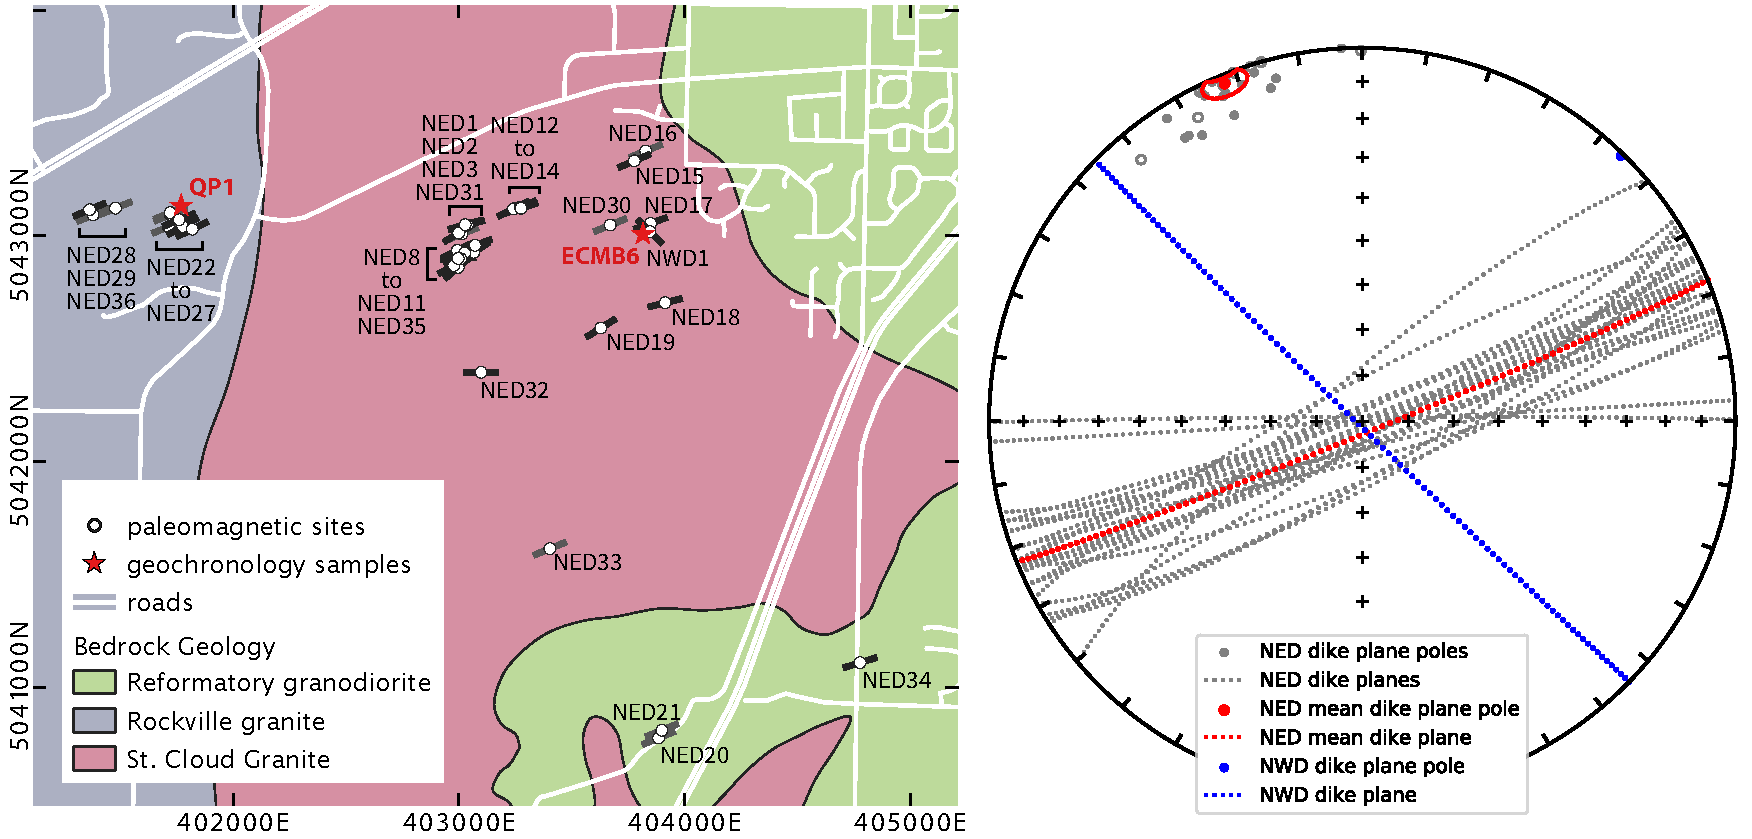
\includegraphics[width=\textwidth]{./figures/map_sites.pdf}
\caption{\setstretch{0.7}\small{Left panel: Locations of paleomagnetic sites of the northeast-trending dikes (NED) and a northwest-trending dike (NWD) within the Rockville Granite, Reformatory Granodiorite and St. Cloud Granite of the ECMB (bedrock geology from \citeA{Boerboom1995a} and shown in UTM zone 15N WGS 84 coordinate reference system such that each axis tick is 1 km). Within regions of the mapped St. Cloud Granite there is more complex interfingering of that granite with the Reformatory Granodiorite than is shown. The strikes of the dikes are shown as lines (black when measured on that dike; grey when using the overall mean orientation from the measured NED dikes). The location of the QP1 and ECMB6 geochronology samples are shown. The ECMB4 geochronology sample was collected $\sim$18 km SW of the western edge of the map, in the Richmond Granite which cross-cuts the Rockville Granite and is younger than the NED dikes. Right panel: The orientations of dikes. Each individual dike orientation is the mean of multiple measurements on that dike. The mean of the poles to the NED planes is shown with a red dot and a 95$\%$ confidence ellipse on the mean calculated with Fisher statistics. This confidence ellipse intersects the equator indicating that the mean plane cannot be distinguished from vertical.}}
\label{fig:site_map}
\end{figure}

\section{Paleomagnetic Methods and Results}

Oriented samples for paleomagnetism were collected and analyzed from 36 of the northeast-trending dikes of the ECMB and one northwest-trending dike (Fig. \ref{fig:site_map}). Each sampled dike constituted a paleomagnetic site in our site naming scheme. These sites were concentrated in and around Stearns County Quarry Park near the city of St. Cloud (Fig. \ref{fig:site_map}). Samples were collected from the dikes with a gas-powered drill and oriented in the field with a Pomeroy orienting fixture. The azimuthal orientations of the cores were determined either through sun or magnetic compass depending on cloud cover. Sun compass directions were preferentially used when available. When magnetic compass data were used they were corrected for local magnetic declination using the International Geomagnetic Reference Field model \cite{Thebault2015a}. Specimens from the oriented samples were analyzed in the UC Berkeley Paleomagnetism lab using a 2G DC-SQUID magnetometer. Samples either underwent stepwise alternating field (AF) or thermal demagnetization. Thermal demagnetization was accomplished using an ASC thermal demagnetizer (residual fields $<$10 nT). AF demagnetization was conducted with inline coils that utilize a Crest Amplifier paired with an Adwin controller to develop a well-controlled waveform. All paleomagnetic data developed in this study are available at the measurement level in the MagIC database (https://www.earthref.org/ MagIC/ doi/ INSERTDOI; UPDATE TO DOI WHEN ASSIGNED).

\begin{figure}[!ht]
\noindent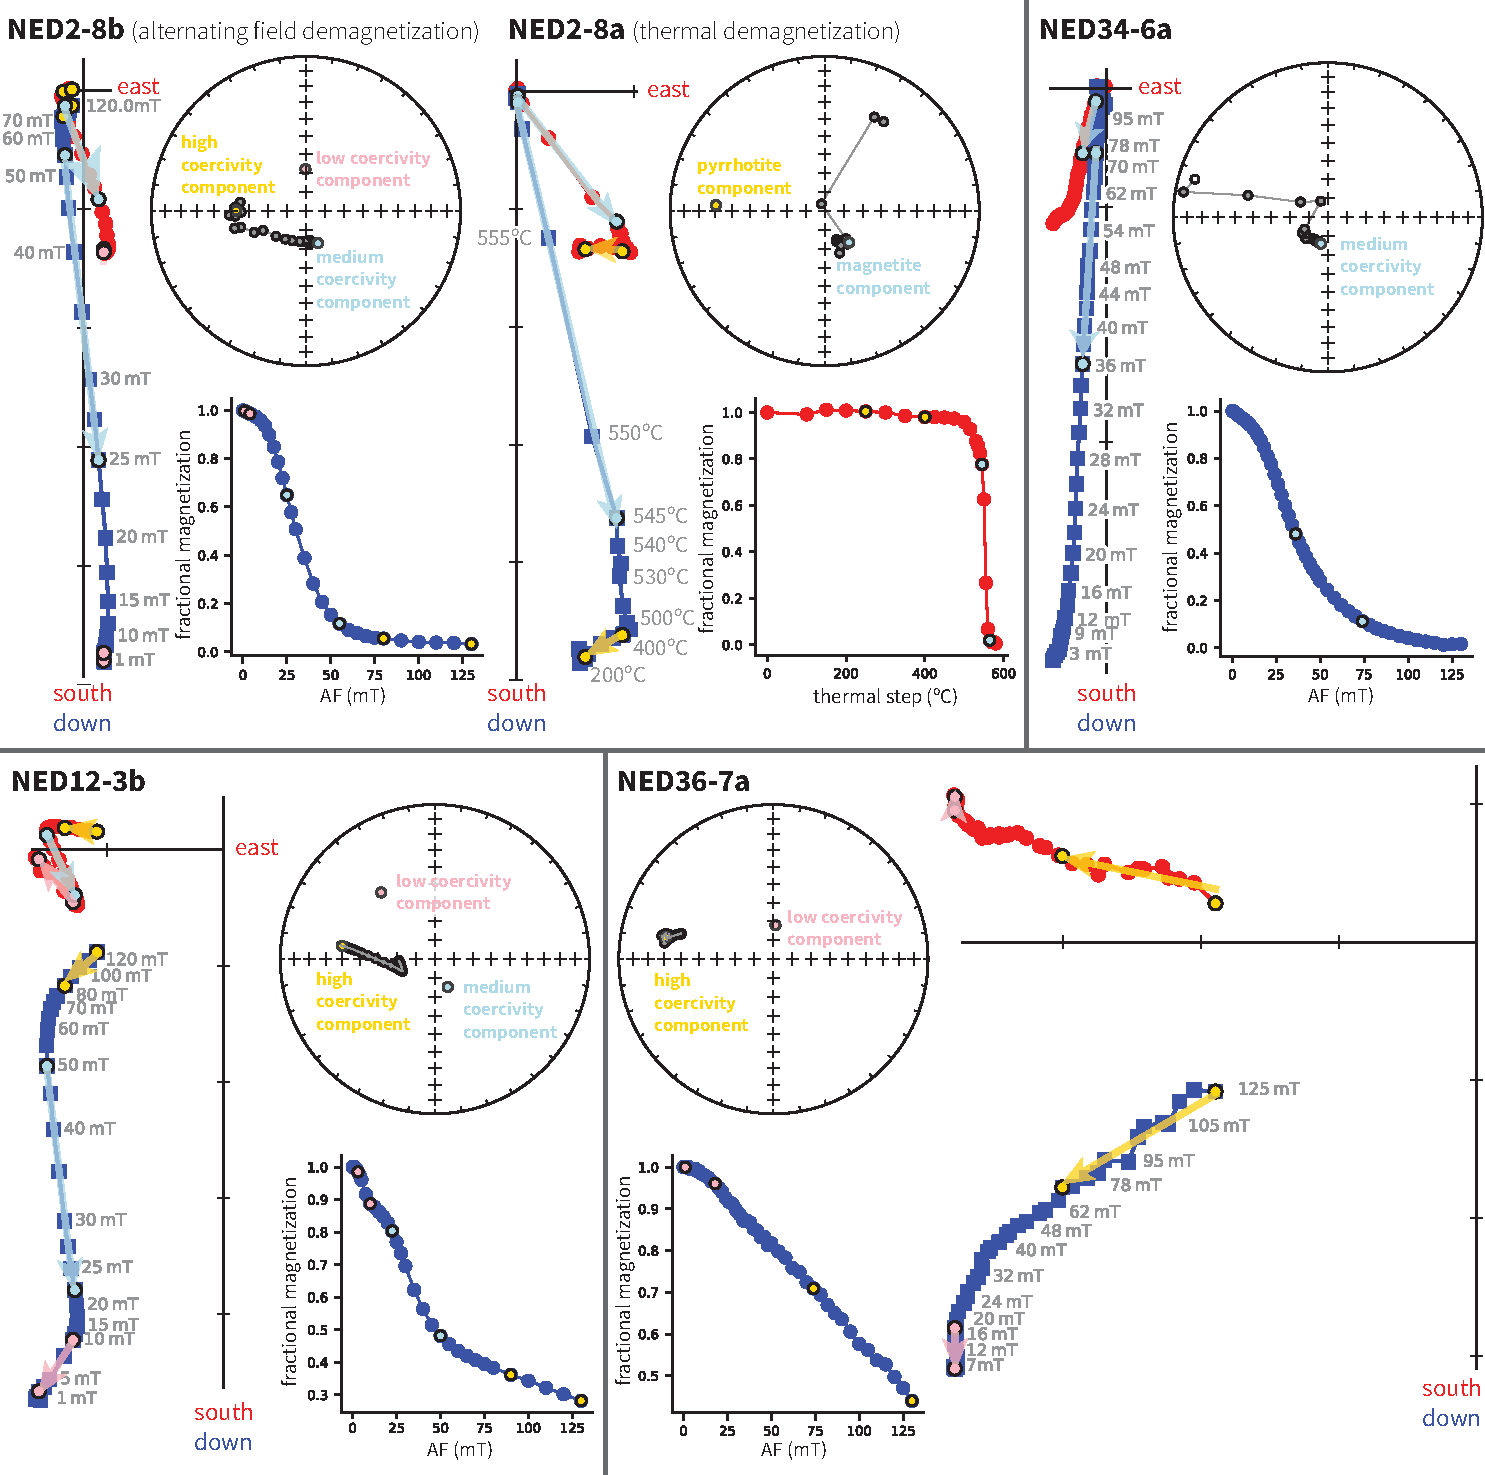
\includegraphics[width=\textwidth]{./figures/paleomag_data.pdf}
\caption{\setstretch{0.7}\small{Paleomagnetic data from ECMB northeast-trending diabase dikes are shown in geographic coordinates on vector component plots, measurement-level equal area plots and magnetization magnitude plots (developed using PmagPy software; \citeA{Tauxe2016a}). Least-squares fits to the data are shown with colored arrows on the vector component plots, colored directions on the equal area plots, and as colored end-points on the magnetization magnitude plots (pink for low-coercivity; blue for medium-coercivity; yellow for high-coercivity). Specimens NED2-8a and NED2-8b are from the same core sample and were analyzed via thermal and alternating field (AF) demagnetization respectively. These data from sample NED2-8 reveal the steep medium-coercivity component to thermally unblock at temperatures characteristic of remanence held by magnetite and the high-coercivity component to thermally unblock at temperatures characteristic of pyrrhotite. Specimen NED34-6a is dominated by the steep medium-coercivity component. The medium-coercivity component is well-resolved in specimen NED12-3b which also has a substantial high-coercivity component. The high-coercivity component dominates the remanence of specimen NED36-7a such that no medium-coercivity component can be resolved.}}
\label{fig:example_pmag}
\end{figure}

Typical behaviors of sample remanence during demagnetization are illustrated for representative specimens in Figure \ref{fig:example_pmag}. AF demagnetization data typically reveal three components: a small low-coercivity component approximately aligned with Earth's present local field in the study region that was typically removed below 10 mT; a medium-coercivity component that is steep and was dominantly removed between 10 and 60 mT; and a high-coercivity component that was subsequently removed incompletely as demagnetization progressed to 130 mT. These components are present to varying degrees within individual specimens (Fig. \ref{fig:example_pmag}).

Sister specimens from some samples underwent thermal and AF demagnetization which provides additional insight into the carriers of the components through comparison of the thermal and AF demagnetization spectra (such as NED2-8 in Fig. \ref{fig:example_pmag}). These data reveal that the low-coercivity component direction is removed at the lowest unblocking temperatures up to 150\textdegree C. This behavior, as well as the typical direction, is most consistent with the component being a viscous overprint acquired in Earth's geomagnetic field. The direction of the high-coercivity component is removed through thermal demagnetization between 250\textdegree C and 350\textdegree C --- consistent with it being held by monoclinic pyrrhotite. The direction of this magnetization held by pyrrhotite is aligned with the magnetite-held remanence within a northwest-trending dike in the region (discussed in more detail below) --- a direction consistent with the position of Laurentia during the time period of \textit{ca.} 1096 Ma Midcontinent Rift magmatism \cite{Swanson-Hysell2020a}. We interpret this high-coercivity component held by pyrrhotite, whose presence is variable in ECMB dikes, to have formed through hydrothermal activity associated with Midcontinent Rift magmatism such as that represented by the emplacement of the northwest-trending dike. The pyrrhotite thereby carries a chemical remanent magnetization.

In some specimens, the low-coercivity component is much larger and has a direction that is distinct from the present local field. It is likely that these samples acquired an isothermal remanent magnetization associated with quarrying operations or lightning strikes. This behavior can be prevalent throughout a site or can be present in just some samples from a given site. In many cases, these low-coercivity overprints can be removed through AF demagnetization and the medium-coercivity and/or high-coercivity components can be subsequently isolated. In some instances, however, these large and dominantly low-coercivity overprints extend to higher coercivities preventing the isolation of other components.

The medium-coercivity component direction is dominantly removed through thermal demagnetization between 515\textdegree C and 565\textdegree C consistent with it being held by low-Ti titanomagnetite. This direction was recovered with site mean direction uncertainty less than 8 degrees ($\alpha_{95}<8^{\circ}$) for 23 sites (Table \ref{tab:pmag_sites}). We interpret this component to be a primary thermal remanence acquired at the time of dike emplacement as part of the \textit{ca.} 1780 Ma ECMB. This interpretation gains support from the rock magnetic data, an inverse baked contact test, and thermochronology data that support an emplacement temperature well below the blocking temperature of magnetite and a mild subsequent thermal history --- as discussed in more detail below. 

\subsection{Magnetic mineralogy constraints from low-temperature magnetometry}

To gain additional insight into the magnetic mineralogy of the dikes, a Magnetic Properties Measurement System (MPMS) at the Institute for Rock Magnetism was used to conduct low-temperature remanence experiments. In the field-cooled (FC) experiments shown in Figure \ref{fig:MPMS_data}, the magnetization was measured upon warming following the specimen having cooled in an applied field of 2.5 T from 300 to 10 K. In the zero-field-cooled (ZFC) experiment, a low-temperature saturation isothermal remanence (LTSIRM) of 2.5 T was applied at 10 K after the specimen cooled in a (near-)zero field. In the room-temperature saturation isothermal remanence (RTSIRM) experiment, the sample was pulsed with a 2.5 T field at room temperature ($\sim$300 K) and then cooled to 10 K and warmed back to room temperature in a (near-)zero field. These experiments reveal that sister specimens to paleomagnetic specimens whose remanence is dominated by the medium-coercivity component without an appreciable high-coercivity component have strong expressions of the $\sim$120 K Verwey transition as expected for a ferromagnetic mineralogy of well-preserved low-Ti titanomagnetite (NED34-6c in Fig. \ref{fig:MPMS_data}; \citeA{Verwey1939a,Feinberg2015a}). In contrast, specimens from samples that have a larger contribution of the high-coercivity component have weaker saturation magnetization, minor expression of the Verwey transition, and the presence of monoclinic pyrrhotite as evidenced through the $\sim$30 K Besnus transition (NED36-8c in Fig. \ref{fig:MPMS_data}; \citeA{Besnus1964a,Feinberg2015a}). Samples with a smaller contribution of the high-coercivity component superimposed on the medium-coercivity component have intermediate behavior with a minor expression of the Besnus transition and a more prominent Verwey transition (NED2-8c in Fig. \ref{fig:MPMS_data}). These results support the interpretation that the medium-coercivity component is held by primary unaltered (titano)magnetite and that the high-coercivity component is the result of subsequent alteration that resulted in degradation of magnetite and formation of pyrrhotite.

\begin{figure}[!ht]
\noindent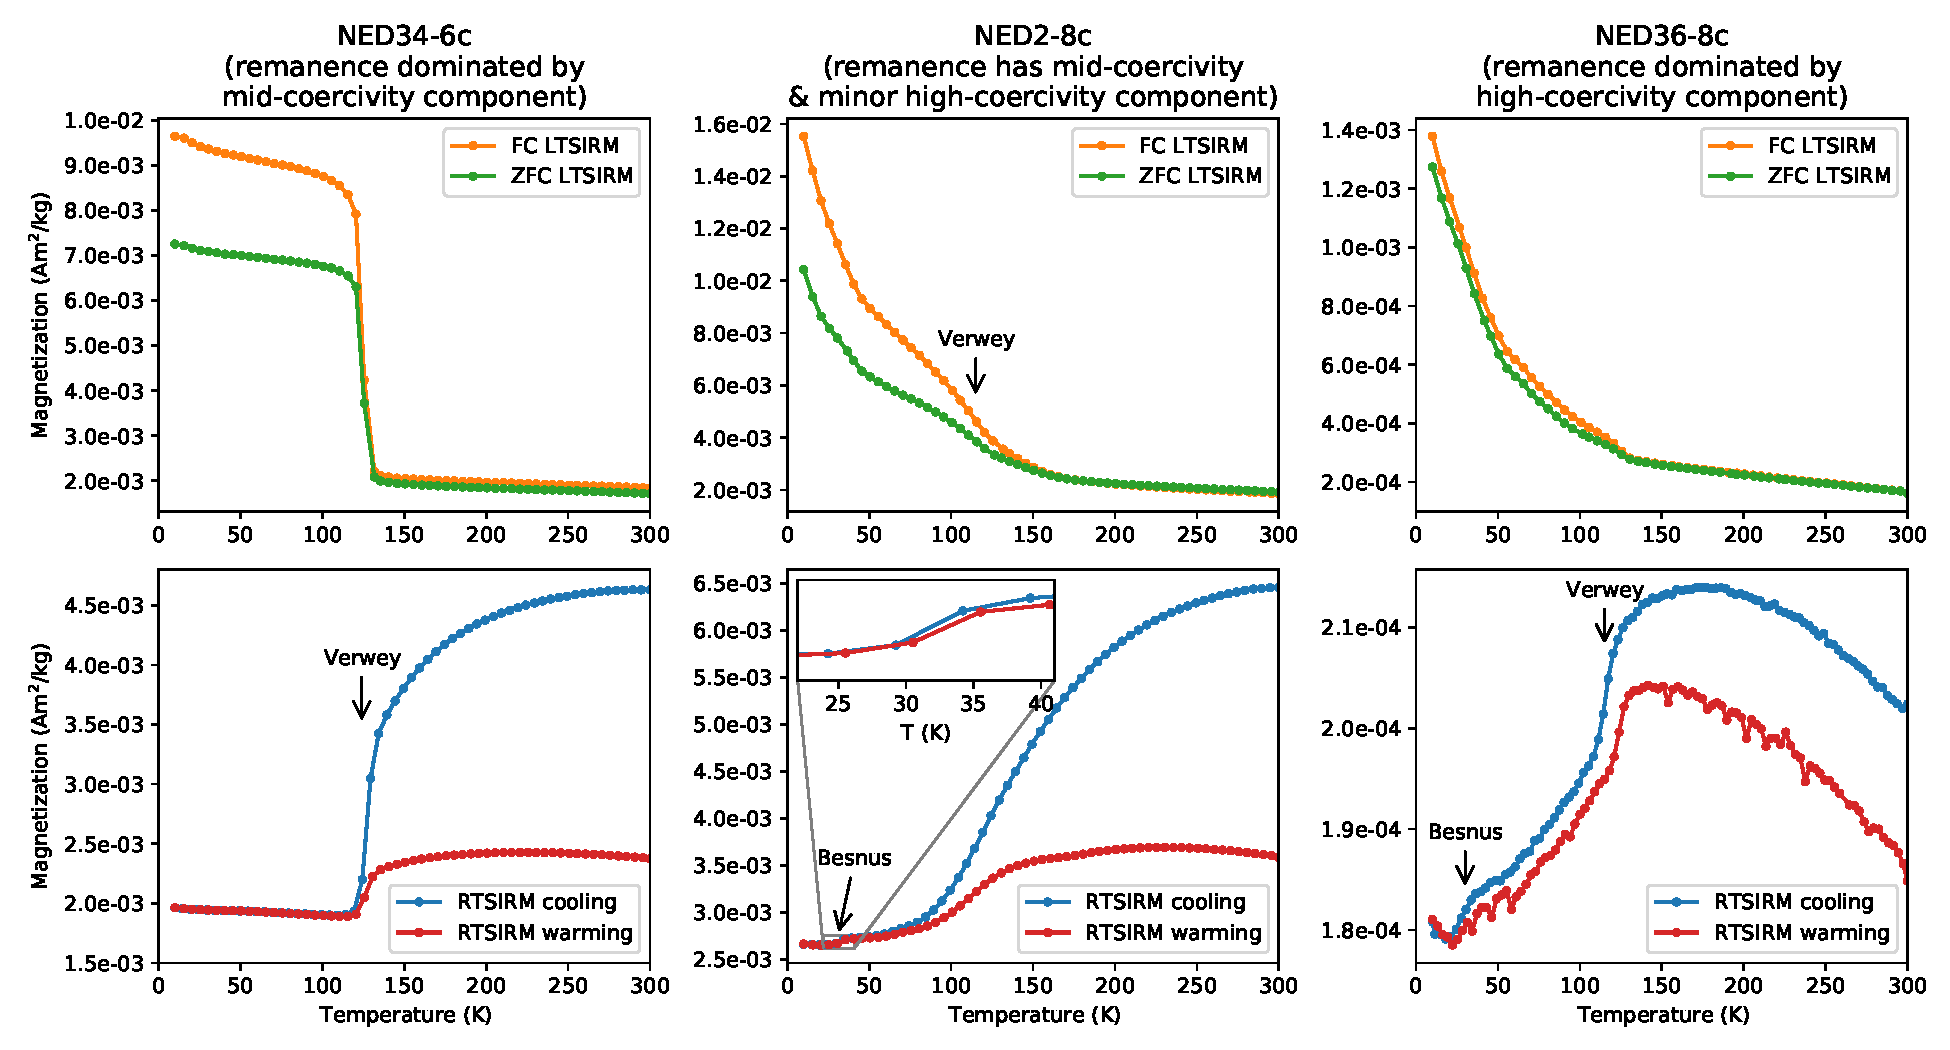
\includegraphics[width=\textwidth]{./figures/MPMS_data.pdf}
\caption{\setstretch{0.7}\small{Low-temperature remanence experiment data. The specimen from a sample whose natural remanent magnetization is dominated by the medium-coercivity component (NED34-6c) has behavior dominated by magnetite as evidenced through the response across the $\sim$120 K Verwey transition. The specimen from a sample whose natural remanence is dominated by the high-coercivity component (NED36-8c) has weaker magnetization, a relatively minor expression of the Verwey transition, and expression of the $\sim$32 K Besnus transition that indicates the presence of monoclinic pyrrhotite. The specimen whose natural remanence has a well-resolved medium-coercivity component with a minor high-coercivity component (NED2-8c) has intermediate behavior with a Verwey transition that is not as suppressed as in NED36-8c with a minor, but resolvable, Besnus transition (see inset). FC: field-cooled; ZFC: zero-field-cooled; LTSIRM: low-temperature saturation isothermal remanence magnetization; RTSIRM: room-temperature saturation isothermal remanence magnetization.}}
\label{fig:MPMS_data}
\end{figure}

\subsection{Baked contact test}

One northwest-trending dike is exposed and was sampled within the study region as site NWD1 (Fig. \ref{fig:site_map}). The magnetization direction of this dike indicates that it is associated with the main stage of the Midcontinent Rift (\textit{ca.} 1096 Ma) as it has a normal polarity and an inclination consistent with that time interval of Midcontinent Rift volcanism (Fig. \ref{fig:baked_contact}; \citeA{Swanson-Hysell2020a}). The dike cross-cuts one of the northeast-trending dikes (NED17) allowing for a baked contact test (Figs. \ref{fig:site_map} and \ref{fig:baked_contact}). The baked contact test is positive with a distinct direction in the northeast-trending dike (corresponding to the remanence direction seen throughout the northeast-trending dikes of the ECMB) with its magnetite remanence becoming progressively overprinted by the northwest-trending dike up to the contact (Fig. \ref{fig:baked_contact}). This positive baked contact test indicates that the northeast-trending ECMB dikes have not been overprinted since the northwest-trending dike was emplaced (\textit{ca.} 1096 Ma). This positive baked contact test for the northwest-trending dike constitutes what is referred to as a positive ``inverse'' baked contact test for the northeast-trending dike remanence --- it constrains the remanence to be more ancient than the \textit{ca.} 1.1 Ga Mesoproterozoic northwest-trending dike, but does not provide a constraint back to the Paleoproterozoic time of dike emplacement. Given that the host rocks for the northeast-trending dikes are of a very similar age to the dikes themselves there is not the possibility of a Paleoproterozoic baked contact test. In contrast to the dikes, stable and consistent remanence directions were not recovered from pilot sites in ECMB granites. 

The high-coercivity remanence direction held by pyrrhotite in some of the northeast-trending dikes is aligned with the remanence direction of the northwest-trending dike. While the thermal effect of the northwest-trending dike was limited to a few meters on either side of it as evidenced through the baked contact test (Fig. \ref{fig:baked_contact}), there was more widespread hydrothermal alteration associated with Midcontinent Rift magmatic activity that led to the formation of pyrrhotite and an associated chemical remanent magnetization. In the majority of the northeast-trending dikes, the original magnetite is well-preserved (e.g., NED34 of Figs. \ref{fig:example_pmag} and \ref{fig:MPMS_data}) while other dikes experienced variable magnetite alteration and the formation of secondary pyrrhotite (e.g., NED36 of Figs. \ref{fig:example_pmag} and \ref{fig:MPMS_data}). These components can be separated through progressive demagnetization (e.g., NED12 of Figs. \ref{fig:example_pmag}) enabling the thermal remanent magnetization held by magnetite to be used to determine site mean directions and calculate a paleomagnetic pole (Fig. \ref{fig:site_means}).

\begin{figure}[!ht]
\noindent\includegraphics[width=\textwidth]{./figures/paleomag_baked_contact_test.pdf}
\caption{\setstretch{0.7}\small{Results from a positive baked contact test where a northwest-trending dike (site NWD1) cross-cuts a northeast-trending dike (site NED17). The NWD1 dike has a direction indicating that it formed during the \textit{ca.} 1096 Ma main stage of rift volcanism. Close to the NWD1 dike the NED17 is nearly fully overprinted (NED17-1a). Further from NWD1 there are partial thermal overprints (NED17-7a) that by $\sim$7 meters from the cross-cutting dike are not resolvable (NED17-11a). Note that blocks from this dike were slightly shifted due to quarrying operations which does not bear on the significance of the positive test, but has led to the exclusion of the result from the site mean compilation and overall pole.}}
\label{fig:baked_contact}
\end{figure}

\subsection{Paleomagnetic pole}

The site mean directions determined from the magnetite remanence component can be converted to virtual geomagnetic poles and then used to calculate a mean paleomagnetic pole for the ECMB diabase dikes (pole longitude: 265.8\textdegree; pole latitude: 20.4\textdegree; A$_{95}$: 4.5\textdegree; K: 45.6 N: 23; Fig. \ref{fig:site_means}). These 23 virtual geomagnetic poles have a distribution consistent with a Fisher distribution as determined through the \citeA{Fisher1987b} goodness-of-fit method. The A$_{95}$ uncertainty on the mean pole position of 4.5\textdegree\ is within the bounds of reliability proposed by \citeA{Deenen2011a}. It is well below the A$_{95}$-max value proposed to establish a well-determined mean for 23 sites (11.4\textdegree) and above the A$_{95}$-min value (3.4\textdegree) consistent with the site directions having sufficiently sampled secular variation of the geomagnetic field.  

In a massive host rock such as the ECMB plutons without preferential bedding or foliation, it is expected that lithospheric stresses will lead to the emplacement of near vertical dikes. Dike plane orientations were measured on each dike for which there was sufficient three-dimensional exposure. Multiple measurements were made for each dike to constrain their orientation. The mean strike calculated from 17 dike orientations is 067\textdegree\ and the mean dip is 88\textdegree\ (Fig. \ref{fig:site_map}). The $\alpha_{95}$ uncertainty associated with the Fisher mean for the poles to these dike orientation planes (i.e. the lines perpendicular to the planes) is 4.7\textdegree\ which means that the overall orientation of the planes is statistically indistinguishable from vertical (Fig. \ref{fig:site_map}). Due to this verticality, we interpret the exhumation of the ECMB plutons to have not resulted in appreciable tilting since dike emplacement and do not apply a tilt correction to the paleomagnetic data.

\begin{figure}[!ht]
\noindent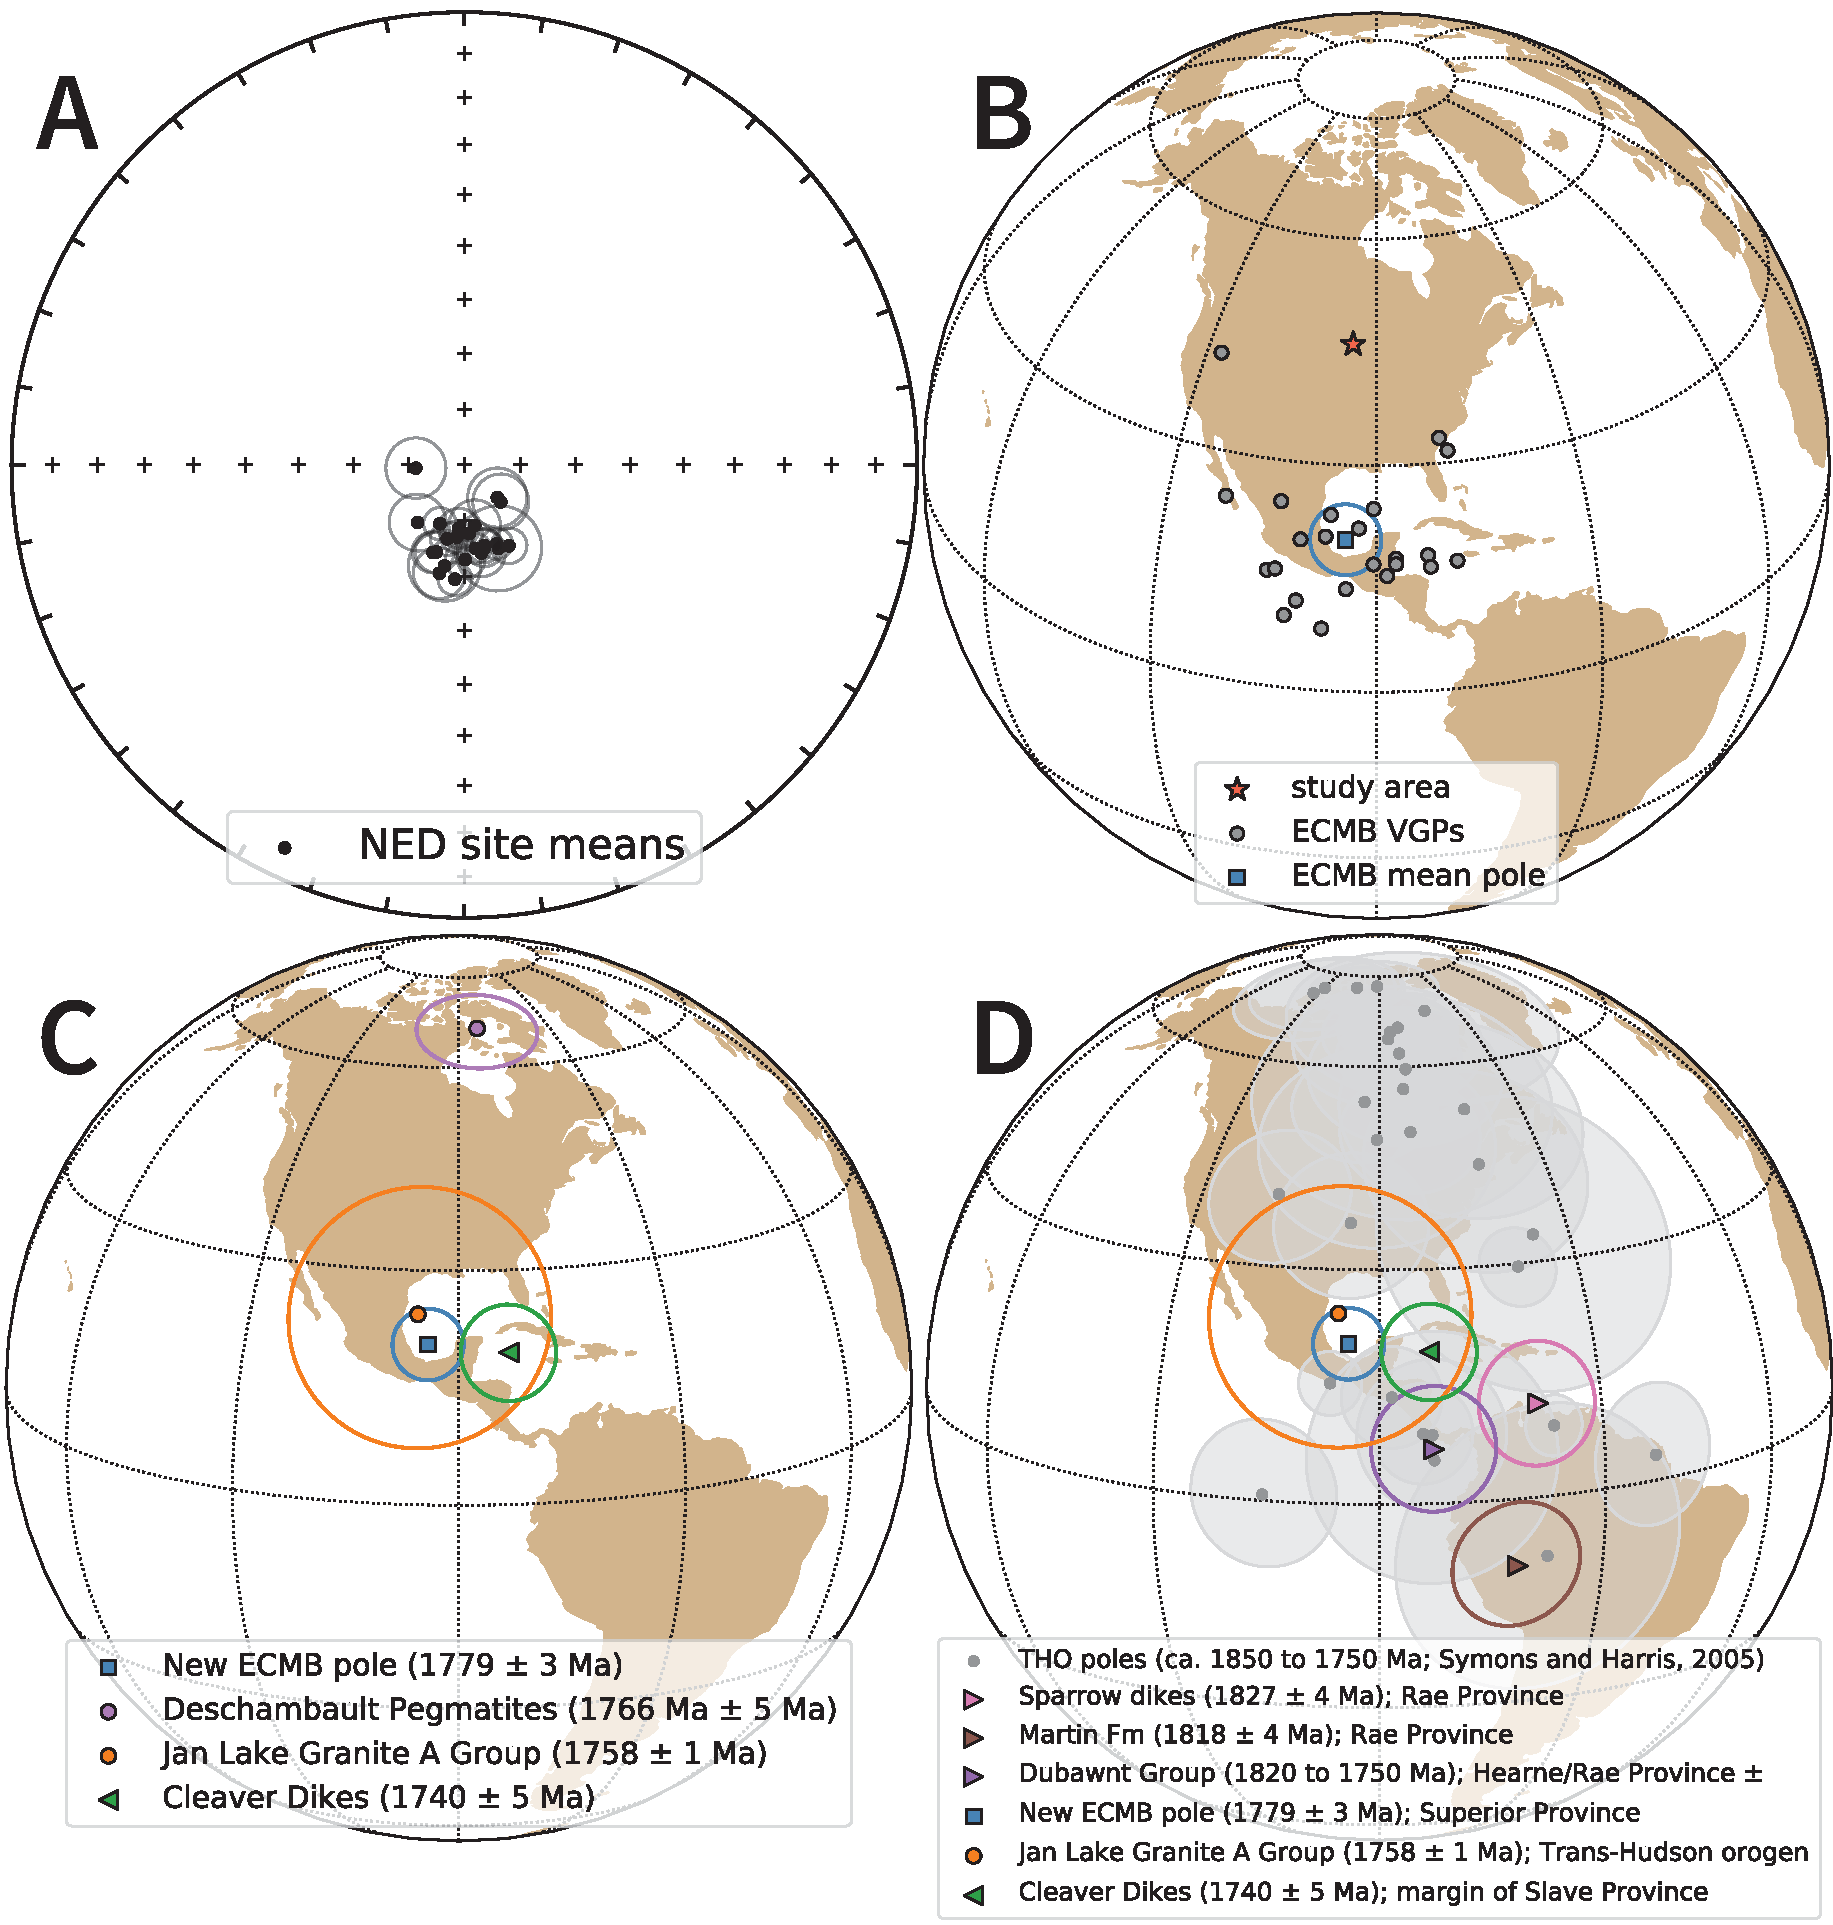
\includegraphics[width=\textwidth]{./figures/paleomag_site_directions_pole.pdf}
\caption{\setstretch{0.7}\small{A) Site mean directions for the magnetite remanence of the northeast-trending (NED) ECMB diabase dikes with $\alpha_{95}<8$\textdegree. B) Virtual geomagnetic poles (VGPs) calculated from these site means and the overall mean paleomagnetic pole for the ECMB dikes. C) Comparison between the new ECMB paleomagnetic pole and other \textit{ca.} 1780 to 1740 Ma poles for Laurentia. D) Comparison of poles from Laurentia's provinces from 1830 to 1740 Ma from \citeA{Evans2021a} as well as poles from the Trans-Hudson orogen (THO; grey; \citeA{Symons2005a}) with the new ECMB pole.}}
\label{fig:site_means}
\end{figure}

\section{Geochronology Methods and Results}

The field relationships show the diabase dikes to be younger than the Rockville Granite, Reformatory Granodiorite and the St. Cloud Granite which they pervasively intrude and to be older than the Richmond Granite where they are absent \cite{Boerboom2005b}. \citeA{Holm2005a} developed U-Pb dates calculated as concordia intercept dates from these intrusions. The dates reported by \citeA{Holm2005a} for granites intruded by the dikes are 1783 $\pm$ 11 Ma for the Reformatory Granodiorite, 1780 $\pm$ 7 Ma for the Rockville Granite and 1779 $\pm$ 5 Ma for the St. Cloud Granite. The younger cross-cutting Richmond Granite has a date of 1772 $\pm$ 3 Ma \cite{Holm2005a}. An age of 1774 $\pm$ 7 Ma for one of the quartz-feldspar porphyry dikes developed by \citeA{Holm2005a} is consistent with this interpretation of these dikes being older than the Richmond Granite (and younger than the granites they intrude). While the dates published in \citeA{Holm2005a} are valuable constraints and are consistent with the field relationships, they are of lower precision than what is possible with modern analytical approaches and therefore lead to overlapping uncertainties. Higher precision constraints resulting from methods that apply ion-exchange separation with low blank analyses of chemically-abraded single zircon grains can test the field relationship interpretations and provide more confidence in the overall age constraints.

\begin{figure}[!ht]
\centering
\noindent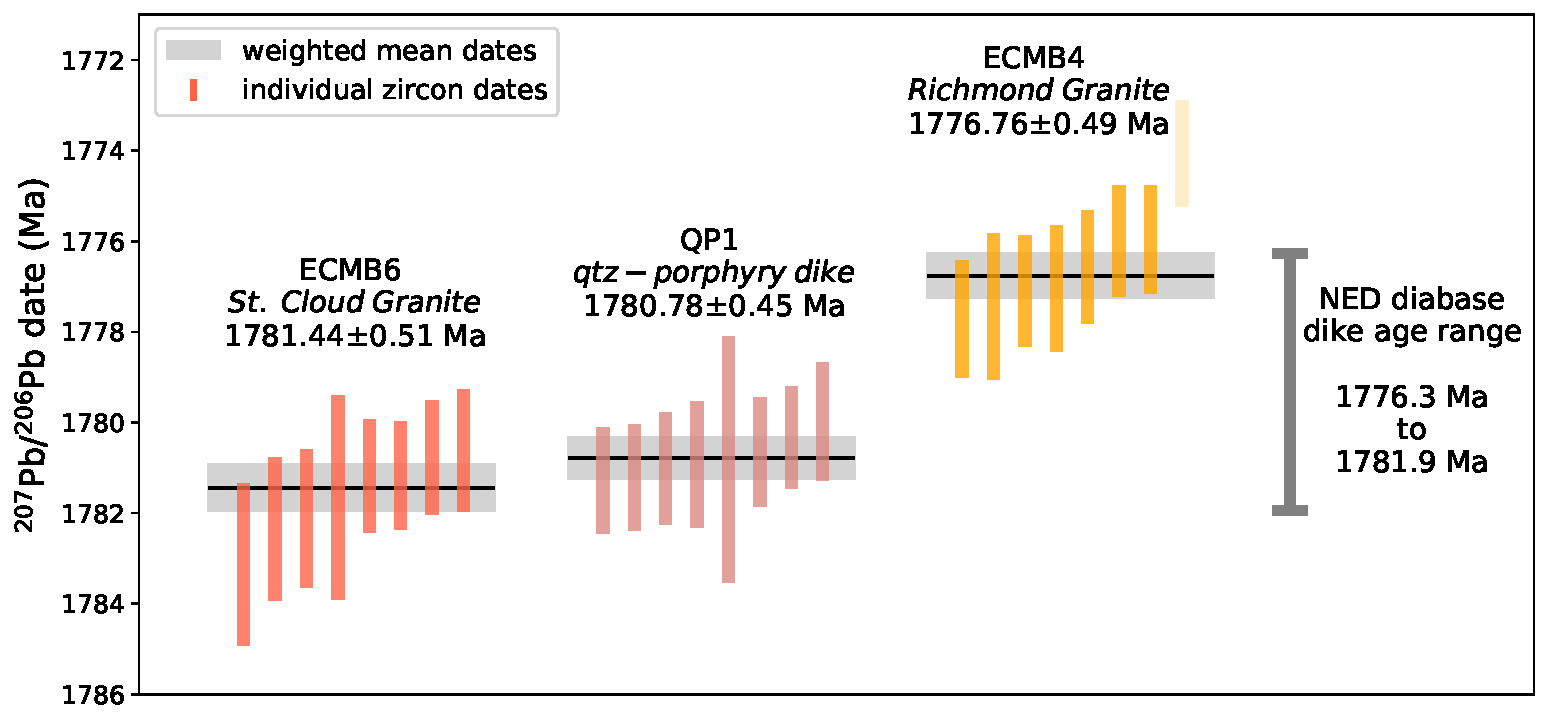
\includegraphics[width=\textwidth]{./figures/ECMB_new_U_Pb_dates.pdf}
\caption{\setstretch{0.7}\small{U-Pb dates for ECMB samples. Weighted mean dates (horizontal lines) are calculated from individual zircon dates (vertical bars). The NED diabase dikes intrude the St. Cloud Granite such that the ECMB6 weighted mean date of 1781.44 $\pm$ 0.51 Ma is a maximum age. The quartz-feldspar porphry dikes (one of which was sampled as QP1) also intrude the St. Cloud Granite and are parallel to the NED diabase dikes. Neither the quartz-porphry dikes nor the diabase dikes intrude the younger cross-cutting Richmond Granite such that the ECMB4 weighted mean date of 1776.76 $\pm$ 0.49 Ma provides a minimum age for the dikes. Details for the weighted mean dates are given in Table \ref{tab:geochron} and individual zircon data are in the Supporting Information.}}
\label{fig:U_Pb_dates}
\end{figure}

To further constrain the age of the northeast-trending diabase dikes, we developed new isotope dilution-thermal ionization mass spectrometry (ID-TIMS) U-Pb zircon dates from the St. Cloud Granite that host the dikes (sample ECMB6), the Richmond Granite from which the dikes are absent (sample ECMB4), and from a northeast-trending quartz-feldspar porphyry dike (sample QP1) that is likely coeval with the diabase dikes (Figs. \ref{fig:site_map} and \ref{fig:U_Pb_dates}). Zircon crystals were chemically abraded prior to analysis of single zircon grains by ID-TIMS at the Boise State Isotope Geology Laboratory (detailed geochronology methods are provided in the Supporting Information). Weighted mean dates were calculated from multiple single zircon dates (Fig. \ref{fig:U_Pb_dates}; Table \ref{tab:geochron}). While chemical abrasion served to reduce Pb-loss and resulted in concordant analyses, some grains have persistent Pb-loss and are discordant (Fig. S1). As a result, we calculate weighted mean  $^{207}$Pb/$^{206}$Pb dates rather than $^{206}$Pb/$^{238}$U dates (Fig. \ref{fig:U_Pb_dates}; Table \ref{tab:geochron}). These $^{207}$Pb/$^{206}$Pb dates are 1781.44 $\pm$ 0.51 Ma (2$\sigma$ analytical uncertainty; MSWD = 1.24; n=8) for the St. Cloud Granite (ECMB6) and 1776.76 $\pm$ 0.49 Ma (MSWD = 1.15; n=7) for the Richmond Granite (ECMB4; Fig. \ref{fig:U_Pb_dates}). The date for the sampled quartz-feldspar porphyry dike (QP1) of 1780.78 $\pm$ 0.45 Ma (MSWD = 0.53; n=8) is between these two dates as expected on the basis of field relationships. Taking into account the analytical uncertainty on the maximum and minimum age constraints, the diabase dikes are younger than the 1781.44 $\pm$ 0.51 Ma St. Cloud Granite and older than the 1776.76 $\pm$ 0.49 Ma Richmond Granite. If one assumes a uniform probability of diabase emplacement timing between the maximum and minimum age constraints that have normally distributed uncertainties, the 95\% confidence interval can be estimated through Monte Carlo simulation. Applying this approach gives a mean age of 1779.1 Ma with 95$\%$ confidence interval (CI) bounds of 1776.8 to 1781.4 Ma. We can succinctly state the age of the northeast-trending ECMB diabase dikes as being 1779.1 $\pm$ 2.3 Ma (95\% CI). 

\section{Thermochronology Methods and Results}

While the U-Pb zircon dates constrain the crystallization ages of the ECMB intrusions, additional insight into the thermal history of the batholith can help with interpretation of the paleomagnetic data given that the thermal remanent magnetization of magnetite will be blocked at temperatures below 580\textdegree C. As discussed below, existing Ar-Ar dates on hornblende and biotite from the ECMB provide valuable constraints in this regard (Fig. \ref{fig:thermochron_dates}). In this study, we also develop new U-Pb apatite dates from three ECMB granites (ECMB1, the Isle Granite; ECMB3, the Rockville Granite; ECMB4, the Richmond Granite). In contrast to zircon, for which the temperatures of appreciable Pb diffusion exceed the liquidus of granite \cite{Cherniak2001a}, the temperature window for closure of the U-Pb system in apatite is much lower ($\sim$ 510 to 460\textdegree C; \citeA{Smye2018a}). As a result, U-Pb dates of apatite serve as a thermochronometer at moderately-high temperatures \cite{Chamberlain2001a, Schoene2007a, Cochrane2014a}. These temperatures are of particular relevance to the interpretation of the paleomagnetic data as they are lower than, or correspond with, the blocking temperature of low-Ti titanomagnetite. If a pluton was emplaced at depths where temperatures exceed the closure temperature of apatite, or if it experienced prolonged reheating, the U-Pb apatite dates would be appreciably younger than the U-Pb zircon crystallization dates.

U-Pb data were developed from apatite grains separated from ECMB granites through laser ablation inductively coupled plasma mass spectrometry (LA-ICP-MS) at UC Santa Barbara (method details are provided in the supporting information). In contrast to zircon, apatite incorporates significant Pb at the time of crystallization. As a result of this elevated common Pb, U-Pb dates were determined through the calculation of Tera-Wasserburg concordia lower intercept dates where the upper intercept corresponds to the ratio of initial $^{207}$Pb/$^{206}$Pb and the lower intercept is the $^{206}$Pb/$^{238}$U date (following the method of \citeA{Ludwig1998a} as implemented in the IsoplotR software of \citeA{Vermeesch2018a}; Fig. S2). Sample ECMB1 is from the Isle Granite which has a U-Pb zircon date of 1779 $\pm$ 26 Ma \cite{Holm2005a}. The U-Pb apatite date for ECMB1 is 1800.3 $\pm$ 33.4/65.2 Ma where the first uncertainty is the 2$\sigma$ analytical uncertainty and the second uncertainty is 95$\%$ confidence interval for the date that incorporates overdispersion (this uncertainty scheme will be used for all the presented apatite dates). This U-Pb apatite date is therefore indistinguishable from the U-Pb crystallization date (Fig. \ref{fig:thermochron_dates}). Sample ECMB3 is from the Rockville Granite which has a U-Pb zircon date of 1780 $\pm$ 7 Ma \cite{Holm2005a}. The U-Pb apatite date for ECMB3 is 1810.5 $\pm$ 16.2/23.0 Ma. The youngest end of the overdispersion uncertainty range is very similar to (albeit just slightly older than) the U-Pb zircon date. It is not geologically reasonable for the U-Pb apatite date to be older than the U-Pb zircon date. This result therefore suggests that the U-Pb apatite date uncertainty is a slight underestimate with the U-Pb apatite system having closed just after the time of zircon crystallization as constrained through the U-Pb zircon date.  Sample ECMB4 is from the Richmond Granite for which we have developed a new ID-TIMS U-Pb zircon date of 1776.76 $\pm$ 0.49 Ma. The U-Pb apatite date for ECMB4 is 1751.7 $\pm$ 17.8/36.6 Ma which is indistinguishable from the U-Pb zircon date (Fig. \ref{fig:thermochron_dates}).

Pb closure temperatures (T$_c$) for the analyzed apatite grains can be estimated with the \citeA{Dodson1973a} approach assuming a cylindrical geometry with half-widths as the characteristic diffusion length. Apatite grain sizes are similar across the three dated specimens; they typically are 100-200 $\mu$m long and 50-75 $\mu$m wide. Using the Pb diffusivity values of \citeA{Cherniak1991a}, a cooling rate of 20\textdegree C/Myr results in closure temperatures of 463\textdegree C to 473\textdegree C for these grain sizes. A more rapid cooling rate is likely for the batholith given the similarity of the U-Pb apatite dates with the U-Pb zircon dates. A cooling rate of 100\textdegree C/Myr from crystallization to apatite closure temperatures results in closure temperatures of 493\textdegree C to 505\textdegree C.

Overall, these data indicate that the samples cooled through the $\sim$500\textdegree C closure temperatures of the U-Pb apatite system near the time of zircon crystallization consistent with rapid cooling rates of the plutons (Fig. \ref{fig:thermochron_dates}). Additionally, there has not been significant diffusion due to later tectonothermal events. As discussed below, this result is consistent with Ar-Ar hornblende dates from the ECMB granites and supports the magnetite remanence being a primary thermal remanent magnetization.

\section{Discussion}

\subsection{Thermal history of the ECMB and a primary interpretation of the ECMB dike pole}

Prior to the emplacement of the ECMB, Paleoproterozoic host rocks were metamorphosed to amphibolite facies during the Penokean orogeny \cite{Holm1990a}. Emplacement of the ECMB has been hypothesized to be post-orogenic and associated with an interval of extensional collapse of the orogen \cite{Holm1996a, Boerboom2000a}. The Al-in-hornblende igneous barometer was applied to the St. Cloud and Isle Granites of the ECMB by \citeA{Holm1998b}. This barometer has varying published calibrations. Applying the pressure calibration of \citeA{Mutch2016a} to the data in \citeA{Holm1998b} and assuming a 2.7 g/cm$^{3}$ overburden gives an estimated emplacement depth of 10.8 $\pm$ 1.7 km for the Freedhem Granodiorite, $\sim$10.4 $\pm$ 1.7 km for the Isle Granite and 13.4 $\pm$ 2.1 km for the St. Cloud Granite. The calibration of \citeA{Ague1997a} leads to slightly higher calculated pressures implying depths that are $\sim$2.3 km deeper. 

\begin{figure}[!ht]
\centering
\noindent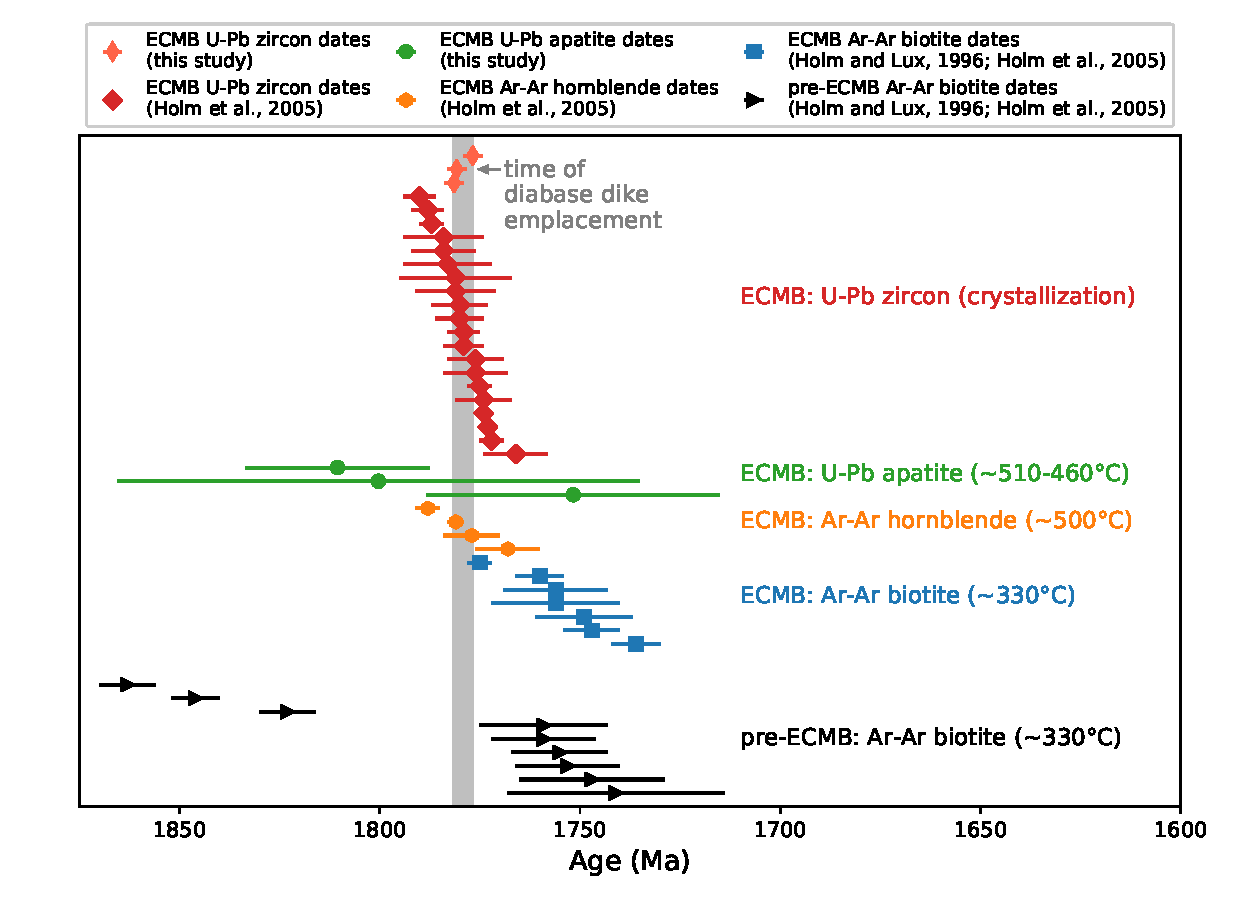
\includegraphics[width=\textwidth]{./figures/ECMB_dates_thermochron.pdf}
\caption{\setstretch{0.7}\small{Summary of U-Pb zircon dates, U-Pb apatite dates, Ar-Ar hornblende, and Ar-Ar biotite dates from the East-Central Minnesota batholith (ECMB) from this study, \citeA{Holm1996a} and \citeA{Holm2005a}. Approximate closure temperatures associated with the thermochronometers are labeled next to the relevant data. That the U-Pb apatite and Ar-Ar hornblende dates are indistinguishable from the U-Pb zircon crystallization dates indicates that the plutons were emplaced at upper middle to upper crustal levels. The Ar-Ar biotite dates from both the ECMB plutons and older host rock lithologies indicate exhumation within $\sim$20 million years to shallower depths and a lack of regional tectonothermal activity over the following 1.75 billion years.}}
\label{fig:thermochron_dates}
\end{figure}

Thermochronology data give additional insight into emplacement temperatures (and thereby depth). Both the Ar-Ar hornblende dates published by \citeA{Holm2005a} and the U-Pb apatite dates developed in this study from ECMB lithologies are indistinguishable from the crystallization ages of the intrusions (Fig. \ref{fig:thermochron_dates}). The closure temperature for Ar in hornblende is $\sim$580 to 490\textdegree C \cite{Harrison1982a}. The closure of the U-Pb system in the dated apatite grains is $\sim$500 to 460\textdegree C. The consistency between the U-Pb zircon crystallization and the U-Pb apatite and Ar-Ar hornblende cooling dates indicates that the present-day erosion level of the ECMB was at a shallow enough depth that the crustal temperatures were lower than these closure temperatures at the time of emplacement of the plutons. Geothermal gradients in continental arc settings are typically between 25 to 45\textdegree C/km -- potentially higher at 1.8 Ga \cite{Rothstein2003a}. Taking a geothermal gradient of 30\textdegree C/km and the closure temperature constraints indicates that the plutons were emplaced at 15 km or shallower in the continental lithosphere. This emplacement depth is consistent with the Al-in-hornblende paleobarometry estimates. 

Ar-Ar biotite dates provide insight into even lower temperatures as the system blocks at $\sim$330\textdegree C \cite{Grove1996a}, well below the blocking temperature of magnetite magnetization in the dikes. Ar-Ar biotite dates from ECMB plutons range from overlapping the crystallization dates to being younger by $\sim$20 million years (Fig. \ref{fig:thermochron_dates}). Ar-Ar biotite dates from older host lithologies to the ECMB are either older than the age of the batholith itself or the same age as the Ar-Ar biotite dates from the batholith (Fig. \ref{fig:thermochron_dates}). These data suggest that the batholith was emplaced near the upper depth range estimates from the Al-in-hornblende barometry ($\sim$10 km) and underwent exhumation to below the $\sim$330\textdegree C closure temperature of the K-Ar biotite system soon after emplacement of the plutons. These data also indicate that there has not been reheating or pervasive fluid flow that would have perturbed the Ar-Ar thermochronometers in the granites in the time since initial cooling. The magnetization used to develop the paleomagnetic pole comes from remanence held by low-Ti magnetite that dominantly unblocks between 540 and 560\textdegree C (Figs. \ref{fig:example_pmag} and \ref{fig:baked_contact}). The thermochronology results constrain the rocks to have cooled through the magnetite blocking temperatures at the time that the dikes were emplaced within the batholith and to not have experienced reheating that would have perturbed the thermochronometers. These data support an interpretation that the magnetite remanence within the ECMB dikes is a primary thermal remanent magnetization.

These thermochronology data also demonstrate that following the emplacement of the ECMB there were not regional tectonothermal events with the potential to have thermally modified the magnetization of the magnetite within the ECMB diabase dikes. Subsequent Paleoproterozoic Yavapai and Mazatzal accretion occurred to the southeast of the Spirit Lake Tectonic zone on the other side of the Minnesota River Valley promontory ($\sim$160 km south of the study region; Fig. \ref{fig:Laurentia_map}; \citeA{Holm2007b}). In contrast to the northeast-trending dikes in the ECMB, northeast-trending dikes in Wisconsin within \textit{ca.} 1840 Ma plutons were metamorphosed to amphibolite facies associated with such accretionary orogenesis \cite{Holm2019a}. Mazatzal orogeny deformation and metamorphism occurred \textit{ca.} 1650 to 1630 Ma within the juvenile accreted island arc of the Wisconsin Magmatic Terrane \cite{Holm1998c}. The region of the ECMB was not affected by these tectonothermal events (Fig.\ref{fig:Laurentia_map}, \citeA{Holm2005a}). \citeA{Holm2005a} proposed that the voluminous ECMB batholith stabilized the continental lithosphere and prevented the region from being modified during subsequent collisions along the margin. This lack of deformation in the region of the ECMB is further supported by the nearly horizontal bedding of ca. 1.63 Ga siliciclastic sedimentary rocks on either side of the batholith \cite{Holm1998c, Medaris2021a}. In southwestern Minnesota, plutons coeval with the ECMB are overlain by the subhorizontal Sioux Quartzite (Fig. \ref{fig:Laurentia_map}) with the correlative Barron Quartzite of northwestern Wisconsin also being undeformed \cite{Southwick1986a}. This lack of deformation contrasts with correlative Baraboo quartzite south of the Spirit Lake Tectonic Zone ($\sim$400 km from the ECMB) that underwent compressional deformation during subsequent orogenesis \cite{Holm1998c,Medaris2021a}. The Yavapai and Mazatzal terranes were intruded by \textit{ca.} 1470 to 1430 Ma granites of the Eastern Granite Rhyolite Province and there is a sizeable pluton of this age within accreted Penokean rocks in northern Wisconsin (the \textit{ca.} 1470 Ma Wolf River batholith; \citeA{Dewane2007a}). However, the thermal effects of the Wolf River batholith ($\sim$370 km east of the ECMB study area) were limited to a 10-15 km wide contact zone surrounding the intrusion \cite{Holm2019a}. 

The one major subsequent tectonothermal event in the region for which there is localized evidence in the ECMB is the development of the Midcontinent Rift that initiated \textit{ca.} 1109 Ma and in which magmatic activity continued to \textit{ca.} 1084 Ma (Fig. \ref{fig:Laurentia_map}; \citeA{Fairchild2017a, Swanson-Hysell2019a}). While the main rift axis can be inferred from gravity and aeromagnetic anomaly data to be located $\sim$75 km southeast of the study region (Fig. \ref{fig:Laurentia_map}), the studied northwest-trending dike has a magnetization direction that implies that it was emplaced during Midcontinent Rift development \textit{ca.} 1096 Ma (Fig. \ref{fig:baked_contact}). The baked contact test between that dike (NWD1) and the northeast-trending dike that it cross-cuts (NED17), indicates that the thermal effect of the dike emplacement and the Midcontinent Rift in general was localized within the immediate vicinity of that dike (a few meters; Fig. \ref{fig:baked_contact}). However, this Midcontinent Rift magmatic activity did result in local hydrothermal alteration as evidenced by magnetization held by monoclinic pyrrhotite that is variably present through the ECMB dikes and is in the same direction as the magnetization of the northwest-trending dike (Fig. \ref{fig:example_pmag}). This chemical remanent magnetization held by monoclinic pyrrhotite would have formed at relatively low temperatures. Phase relationships in the Fe-S system developed through hydrothermal recrystallization experiments show monoclinic pyrrhotite to form at temperatures below 250\textdegree C and likely above 75\textdegree C \cite{Kissin1982a}. While in some sites, this pyrrhotite-forming alteration obscured the primary thermal remanence held by magnetite (e.g., NED36 in Fig. \ref{fig:example_pmag}), in the majority of sites the magnetite remanence direction can be well-resolved (e.g., NED2, NED12 and NED34 in Fig. \ref{fig:example_pmag}). As a result, the paleomagnetic directions used to calculate the paleomagnetic pole shown in Figure \ref{fig:site_means} are held by (titano)magnetite that recorded a thermal remanent magnetization upon cooling of the diabase dikes. This evidence for variable late Mesoproterozoic hydrothermal alteration of the dikes provides an explanation for Ar-Ar data developed from two northeast-trending diabase dikes that were reported in \citeA{Boerboom2000a}. These Ar-Ar data did not yield a plateau age, but give whole rock total gas dates that are late Mesoproterozoic in age. An interpretation that these whole rock total gas ages correspond with the age of emplacement is difficult to reconcile with the cogenetic relationship between the diabase dikes, the quartz-feldspar porphyry dikes and the ECMB granites. K-Ar whole-rock ages of 1570 to 1280 Ma from the dikes reported in \citeA{Hanson1968a} and discussed in \citeA{Horan1987a} are attributed to partial resetting. The evidence for fluid flow that led to the formation of pyrrhotite \textit{ca.} 1096 Ma supports the hypothesis put forward by \citeA{Horan1987a}, as well as by \citeA{Boerboom2000a}, that there was Mesoproterozoic disruption of the K-Ar isotopic system in the dikes such that the Mesoproterozoic Ar-Ar dates are the result of alteration of dikes which are Paleoproterozoic in age. The field relationships indicating that the northeast-trending diabase dikes are comagmatic with ECMB granites is also consistent with whole rock Pb isotope data that reveal very similar arrays implying a \textit{ca.} 1.8 Ga isochron age for both lithologies \cite{Horan1987a}. 

%The Section 28 Granite from the Minnesota River Valley was precisely dated at ~1781 Ma and also displays impressive comingling textures with mafic enclaves (see fig. 4 in that paper and unit descriptions). Perhaps the occurrence of this similar lithology and date should also be mentioned in the Discussion.

Overall, the constraints requiring that the ECMB granites were emplaced at depths where the ambient temperature was below the closure of U-Pb apatite and Ar-Ar hornblende systems indicate that the comagmatic diabase dikes would have acquired their magnetization at the time of emplacement. The lack of significant thermal events that could have reset the magnetite magnetization is indicated by the geologic setting, the thermochronology data (including the Paleoproterozoic Ar-Ar biotite dates), and the positive inverse baked contact test. We therefore interpret the pole calculated from the magnetite remanence of the ECMB diabase dikes as a high-quality constraint on the paleogeographic position of Laurentia at the time the dikes intruded (1779.1 $\pm$ 2.3 Ma). The ECMB diabase dikes pole meets six of the seven criteria for the quality criteria \citeA{Van-der-Voo1990a} and the \citeA{Meert2020a} reliability criteria with the only one not satisfied being due to the lack of dual polarity directions. This single polarity normal polarity is consistent with the polarity of the Cleaver Dykes and the proposal of \citeA{Irving2004a} that there was a normal geomagnetic superchron that followed the Trans-Hudson orogeny.

\begin{figure}[!ht]
\begin{centering}
\noindent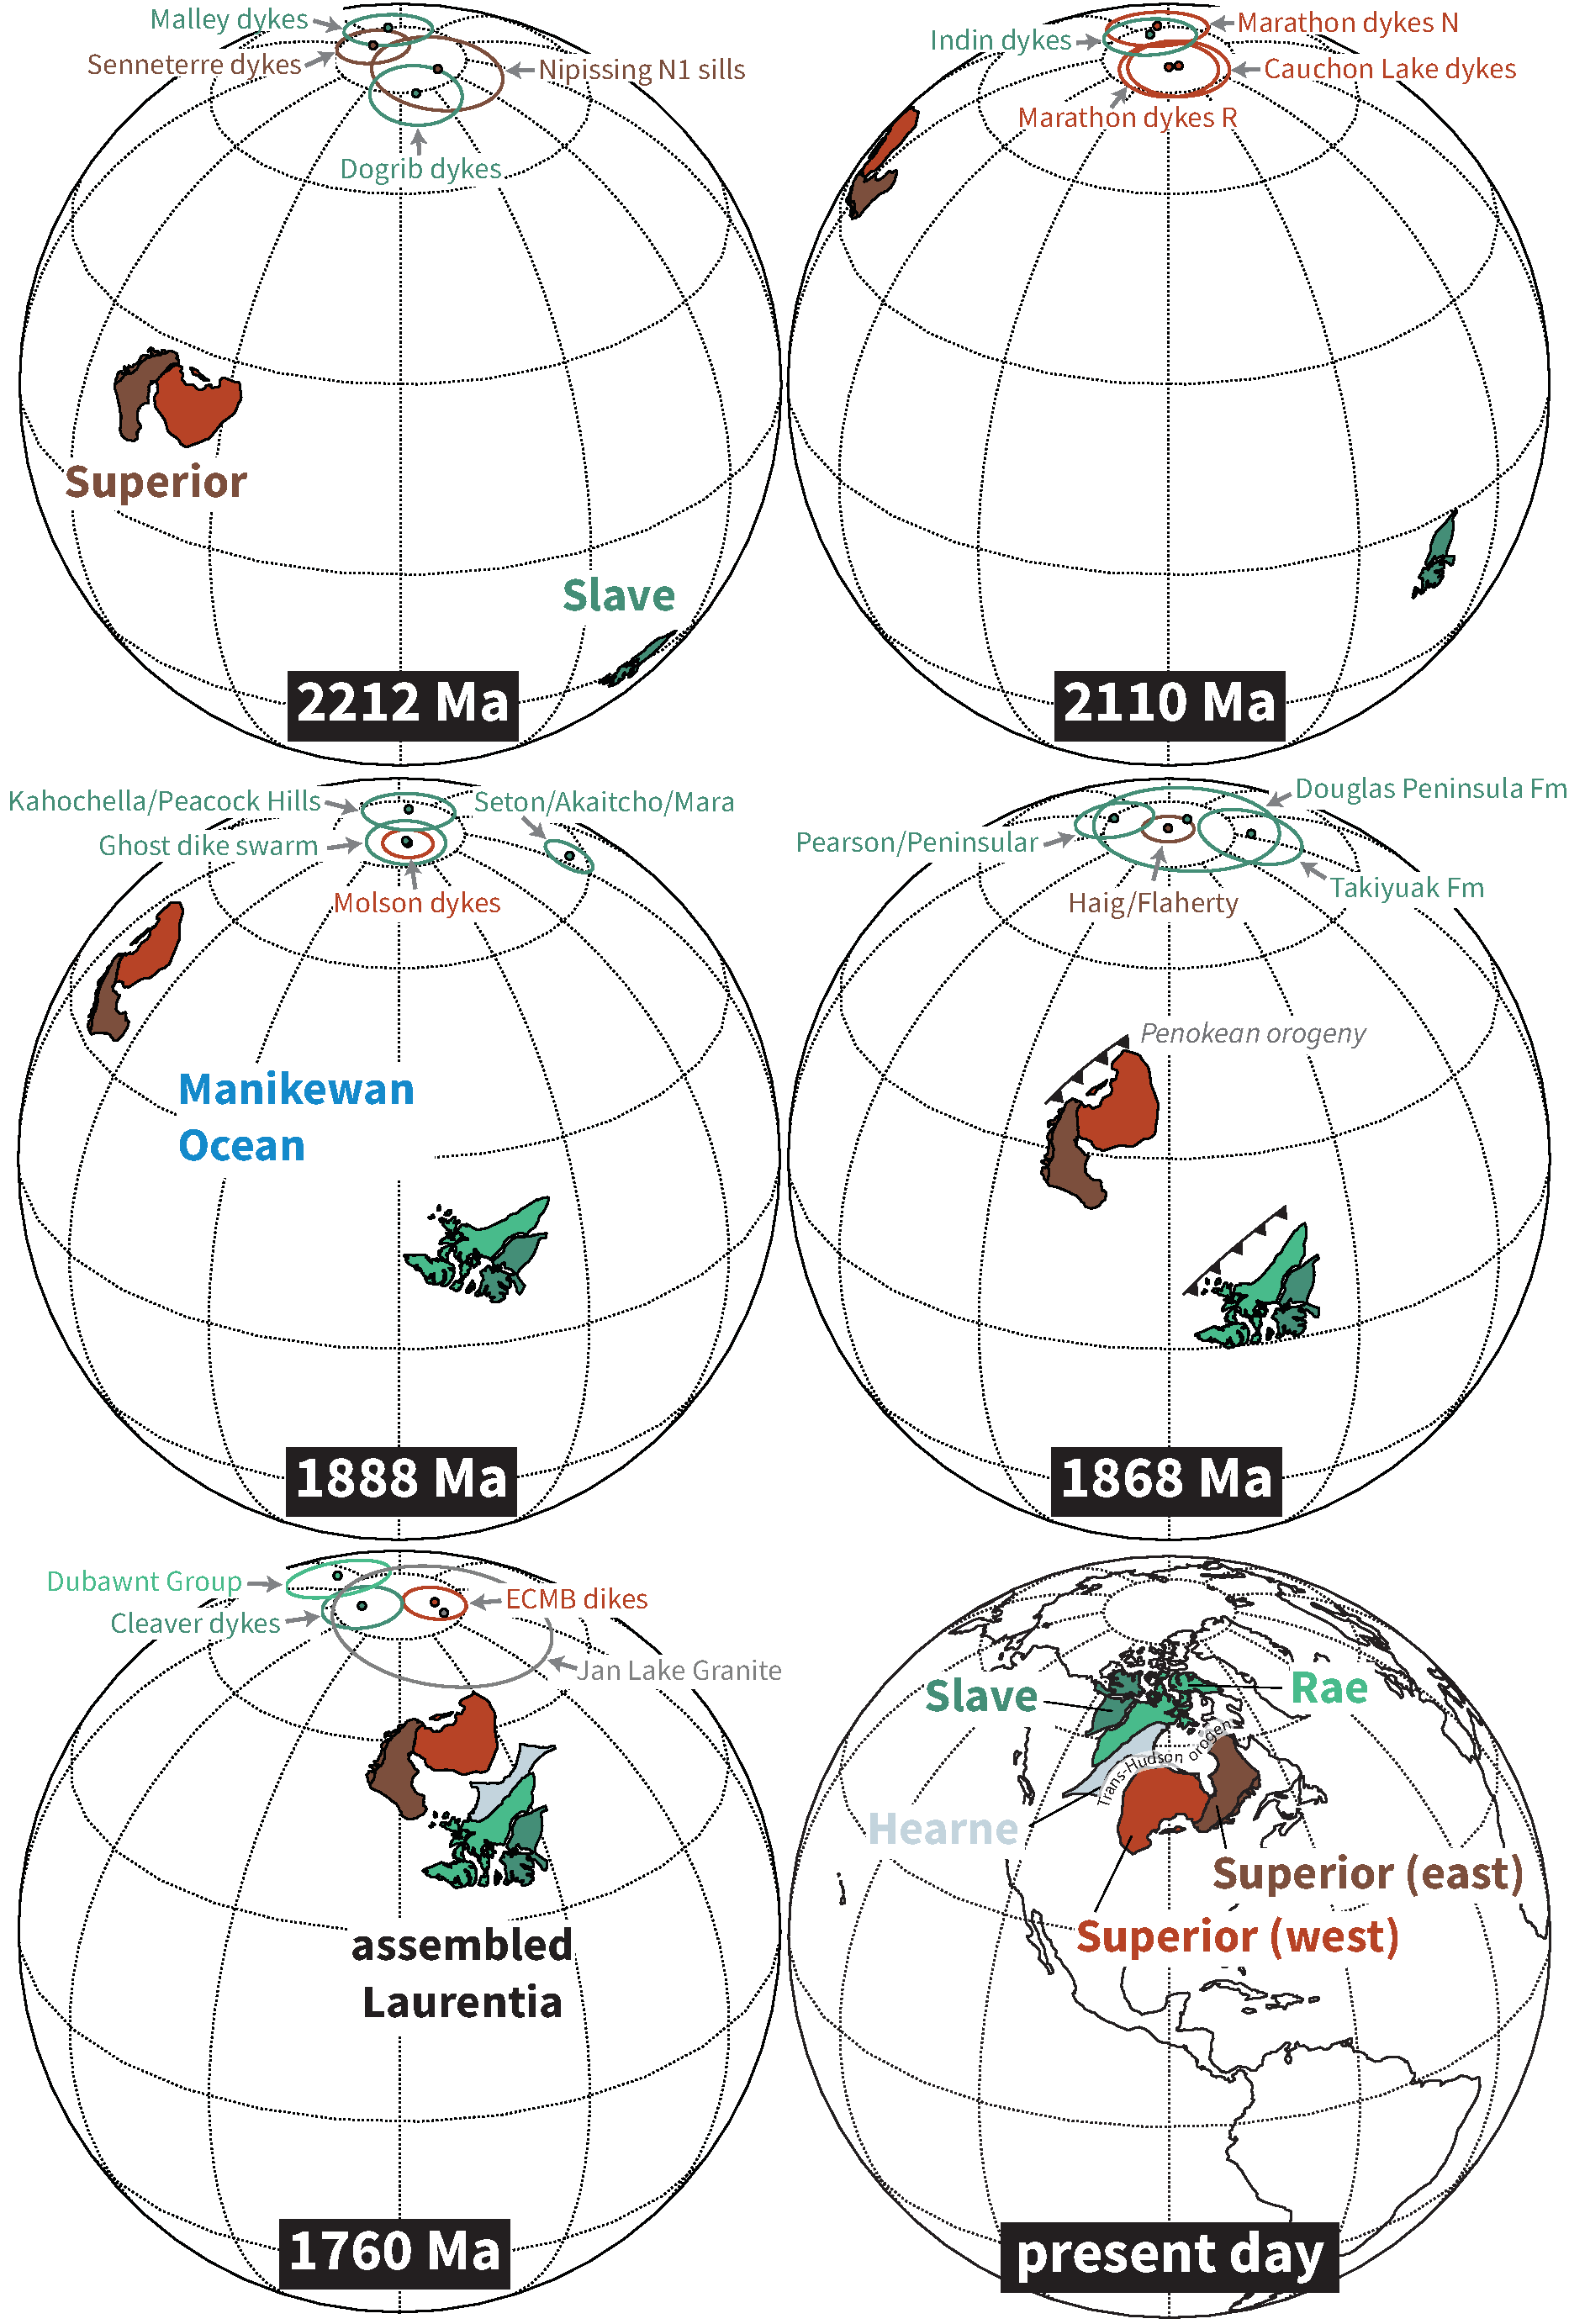
\includegraphics[width=4.65 in]{./figures/paleogeo_reconstruction.pdf}
\caption{\setstretch{0.7}\small{Paleogeographic reconstructions at five different times in the Paleoproterozoic and the position of the provinces at present. Paleomagnetic poles within 20 Myr of the given time (10 Myr for 1888 and 1868 Ma) are shown from the compilation of \citeA{Evans2021a} as well as the new ECMB pole. These data illustrate differential plate motion between the Superior and Slave Provinces that is required by the data leading up to the closure of the Manikewan Ocean and the assembly of Laurentia during the Trans-Hudson orogeny. The ECMB pole is consistent with an assembled Laurentia following the Trans-Hudson orogeny which contrasts with the disparate orientations and paleolatitudes between Laurentia's constituent provinces prior to the orogeny.}}
\label{fig:Superior_Slave_recons}
\end{centering}
\end{figure}

\subsection{Laurentia's paleomagnetic poles following the Trans-Hudson orogeny}

The Trans-Hudson orogeny is a major event in the formation of Laurentia resulting from collision between the Superior province and the Churchill plate consisting of the composite Slave + Rae + Hearne provinces \cite{Hoffman1988a, Corrigan2009a, Weller2017a}. Geologic data on the timing of Trans-Hudson orogenesis include a $^{206}$Pb/$^{238}$U date of 1854.2 $\pm$ 1.6 Ma from the base of a foredeep sedimentary succession on the northern margin of the East Superior province that constrains flexural subsidence associated with Trans-Hudson orogenesis to have initiated at that time \cite{Hodgskiss2019a}. This timing of orogenesis is consistent with $^{207}$Pb/$^{206}$Pb dates of monazite within garnet of Trans-Hudson orogen ecologites for which a mean date of 1831 $\pm$ 5 Ma has been interpreted to record peak metamorphism \cite{Weller2017a}. A similar timing of \textit{ca.} 1860 to 1820 Ma peak Trans-Hudson metamorphism resulting from collisional orogenesis has been interpreted from U-Pb zircon rim and monazite dates from the orogen in Baffin Island, Nunavut, Canada \cite{Skipton2016a}. These geologic data strongly support that the Superior Province was conjoined with the Slave + Rae + Hearne provinces prior to 1800 Ma in their present-day relative positions (Fig. \ref{fig:Laurentia_map}). There are high-quality paleomagnetic poles for the Superior province during the time interval when the Manikewan Ocean was closing leading up to the Trans-Hudson orogeny (the \textit{ca.} 1880 Molson dykes pole and the \textit{ca.} 1870 Ma Haig/Flaherty pole; Fig. \ref{fig:Superior_Slave_recons}). There are no Paleoproterozoic paleomagnetic poles for the Superior Province during or after the Trans-Hudson orogeny that can test Laurentia's coherency with paleomagnetic data. The new 1779.1 $\pm$ 2.3 Ma ECMB paleomagnetic pole fills this gap.

 While abundant paleomagnetic data have been developed from rocks within the Trans-Hudson orogen \cite{Symons2005a}, both the primary nature of the remanence directions as well as the age of remanence acquisition has been challenging to establish. As a result, relatively few poles from this interval during and following Laurentia's amalgamation have been included in curated pole compilations such as that compiled by the Nordic paleogeography workshops \cite{Evans2021a}. The best constrained of these poles comes from the post-orogenic 1740 $\pm$ 5 Ma Cleaver Dykes of the Great Bear Magmatic Arc on the western margin of the Slave Province (Fig. \ref{fig:Laurentia_map}; \citeA{Irving2004a}). The age of these dikes is constrained by a U-Pb baddeleyite date and there is a positive baked contact test supporting the interpretation that the pole is primary. As can be seen in Figure \ref{fig:site_means}, the position of this \textit{ca.} 1740 Ma Cleaver Dykes pole for Laurentia \cite{Irving2004a} is similar to the new pole for the \textit{ca.} 1780 Ma ECMB diabase dikes (Fig. \ref{fig:site_means}). They do not share a common mean (as determined through Watson and bootstrap common mean tests; \citeA{Tauxe2016a}), but are within 11\textdegree\ of one another (less when considering uncertainty). The similarity in these pole positions provides an independent test of the coherency of the Laurentia craton at that time.
 
 An additional pole for comparison comes from hematite remanence of volcanics and sediments of the Baker Lake Group of the Dubawnt Supergroup which were deposited in a basin atop the suture between the Rae and Hearne provinces (Figs. \ref{fig:Laurentia_map} and \ref{fig:site_means}; \citeA{Park1973a}). Both the depositional age of the succession and the age of hematite remanence are roughly constrained leading to a wide assigned age range of 1820 to 1750 Ma in \citeA{Evans2021a} for the pole. While the loose age constraints hinder firm comparisons, the broad similarity of this pole with the Cleaver Dykes pole of the Slave Province as well as that for Martin Formation (1818 $\pm$ 4 Ma) and the Sparrow dikes (1827 $\pm$ 4 Ma) of the Rae Province establishes a largely consistent position of the Churchill plate from \textit{ca.} 1820 to 1740 Ma. 
 
 A less robust pole for comparison with the new ECMB pole comes from the post-orogenic Jan Lake Granite within the Trans-Hudson orogen in southeast Saskatchewan developed in \citeA{Gala1995a}. A U-Pb zircon date of 1758 $\pm$ 1 Ma for this granite was reported in \citeA{Bickford2005a}. Directional data from the Jan Lake Granite falls into two groups. Based on thermal demagnetization behavior, \citeA{Irving2004a} interpreted the `A' grouping to be a TRM held by magnetite that was acquired at the time of the emplacement of the intrusion \textit{ca.} 1758 Ma.  The ECMB dikes pole shares a common mean with this Jan Lake Granite pole with overlapping A$_{95}$ confidence circles (Fig. \ref{fig:site_means}). This result is consistent with both the Jan Lake Granite and ECMB being post-orogenic magmatic events that occurred following the amalgamation of Laurentia. This similarity suggests that despite the large uncertainty on the Jan Lake Granite pole and the ambiguity resulting from multiple directional groups that the pole does constrain the position of Laurentia \textit{ca.} 1758 Ma. 
 
 A pole that does not hold up to such comparative scrutiny is that developed for the Deschambault Pegmatites from within the Trans-Hudson orogen (Fig. \ref{fig:site_means}C; \citeA{Symons2000a}).  This pole has been interpreted to constrain the position of Laurentia \textit{ca.} 1766 Ma --- an age based on U-Pb monazite and allanite dates of other pegmatites in the region. As noted in \citeA{DAgrella-Filho2020a}, there are no field tests for this pole and the remanence directions from which it is calculated are quite close to the modern geomagnetic field. This pole was included in the curated Nordic paleogeography workshop compilation of  \citeA{Evans2021a} less because of the quality of the individual pole, but rather because there are a number poles of similar position to this one from the Trans-Hudson orogen (Fig. \ref{fig:site_means}). Many of these poles have individual VGPs that are streaked between directions similar to the Jan Lake Granite and that of the present-local field. The direction of the Deschambault pole is far from the new \textit{ca.} 1780 Ma ECMB dikes pole. In contrast, the similarity of pole position between the new ECMB dikes pole and the \textit{ca.} 1758 Ma Jan Lake Granite pole as well as the \textit{ca.} 1740 Ma Cleaver Dykes pole supports that these poles, rather than the Deschambault Pegmatites pole, constrain Laurentia's position during this interval. This Deschambault Pegmatites pole played a role, in conjunction with other poles from the Trans-Hudson orogen, such as that from the Wapisu gneiss and the Deschambault Post pluton, in an interpretation that Laurentia's pole path was at a standstill in the vicinity of the Deschambault Pegmatites pole from \textit{ca.} 1800 Ma through to \textit{ca.} 1766 Ma \cite{Symons2000a, Symons2005a}. As reviewed in \citeA{Raub2008a}, there are numerous difficulties in interpreting these data from the Trans-Hudson orogen as useful constraints including: 1) a lack of field tests; 2) uncertainty in the timescale of cooling and the timing of the acquisition of magnetization in these slowly cooled units; 3) poorly constrained tilt corrections and 4) large secondary viscous remanent magnetizations that are prevalent due to the coarse grain-size of the igneous lithologies. The preferred interpretation of \citeA{Raub2008a}, which is echoed in \citeA{DAgrella-Filho2020a}, is that there is unresolved component mixing between primary directions (which would be in the vicinity of the Jan Lake Granite A Group pole and our new ECMB pole) and the present-day north pole as the result of unresolved viscous overprints (Fig. \ref{fig:site_means}). This component mixing leads to streaked site mean directions in individual studies as well as the database of Trans-Hudson orogen poles including the Deschambault Pegmatites pole (Fig. \ref{fig:site_means}; \citeA{Raub2008a}). The new ECMB pole significantly strengthens this interpretation by demonstrating that a proposed northerly apparent polar wander path to satisfy the Deschambault Pegmatites pole and other Trans-Hudson orogen poles streaked between the Jan Lake Granite and the modern-day pole is indeed fictitious (Fig. \ref{fig:site_means}). Instead, the ECMB pole and the Cleaver Dykes pole establish the paleogeographic position of Laurentia to have been consistent \textit{ca}. 1780 to 1740 Ma (Fig. \ref{fig:Superior_Slave_recons}).
 
\subsection{The paleogeography of Laurentia}

As is expected by the geologic record of Trans-Hudson orogenesis, the similarity in pole positions from the southeastern margin of the Superior Provinces (the new ECMB pole) and the northwestern margin of the Slave Province (the Cleaver Dykes pole; Fig. \ref{fig:site_means}) indicate a coherent assembled Laurentia following 1.8 Ga (Fig. \ref{fig:Superior_Slave_recons}). The coherency of the record of high-quality paleomagnetic poles at this time when the geologic record indicates a recently assembled Laurentia increases confidence that differing pole positions between Laurentia's Archean provinces earlier in the Paleoproterozoic are indeed a record of differential plate tectonic motion (Fig. \ref{fig:Superior_Slave_recons}). There is a particularly rich record of paleomagnetic poles from the Archean Superior and Slave provinces that can be paired between 2.23 and 1.89 Ga that constrain the provinces to not be in their modern relative orientation and to be undergoing differential motion \cite{Mitchell2014a, Buchan2016a, Swanson-Hysell2021a}. These poles result in reconstructions where prior to the Trans-Hudson orogeny there was an ocean basin between the Superior province and the Hearne + Rae + Slave provinces known as the Manikewan Ocean (Fig. \ref{fig:Superior_Slave_recons}; \citeA{Stauffer1984a}). The poles are consistent with the Superior Province approaching the joint Slave + Hearne + Rae provinces prior to the onset of the Trans-Hudson orogeny (Fig. \ref{fig:Superior_Slave_recons}). These data provide strong evidence for mobile lid plate tectonics from 2.23 Ga onward \cite{Mitchell2014a, Buchan2016a, Swanson-Hysell2021a}.

The orogenesis associated with Laurentia's assembly is hypothesized to have resulted in the formation of the supercontinent, or semi-supercontinent, Nuna \cite{Hoffman1997a, Evans2011a, Evans2016a}. Given that Laurentia is the largest craton hypothesized to have been part of this supercontinent, its paleogeographic position is key to reconstructions of Nuna. The new ECMB pole provides higher confidence in the paleogeographic position of Laurentia in the time just following its formation from the collision of constituent Archean provinces (Fig. \ref{fig:Superior_Slave_recons}). This new pole can be used to evaluate hypothesized connections between Laurentia and other cratons. There is an increasingly rich global database of paleomagnetic poles \textit{ca.} 1780 Ma including poles from the Amazonia, Baltica, India, Rio de la Plata, S\~{a}o Francisco and North China cratons \cite{Zhang2012a, Xu2014a, Bispo-Santos2014a, Shankar2018a, DAgrella-Filho2020a}.

\begin{figure}[!ht]
\noindent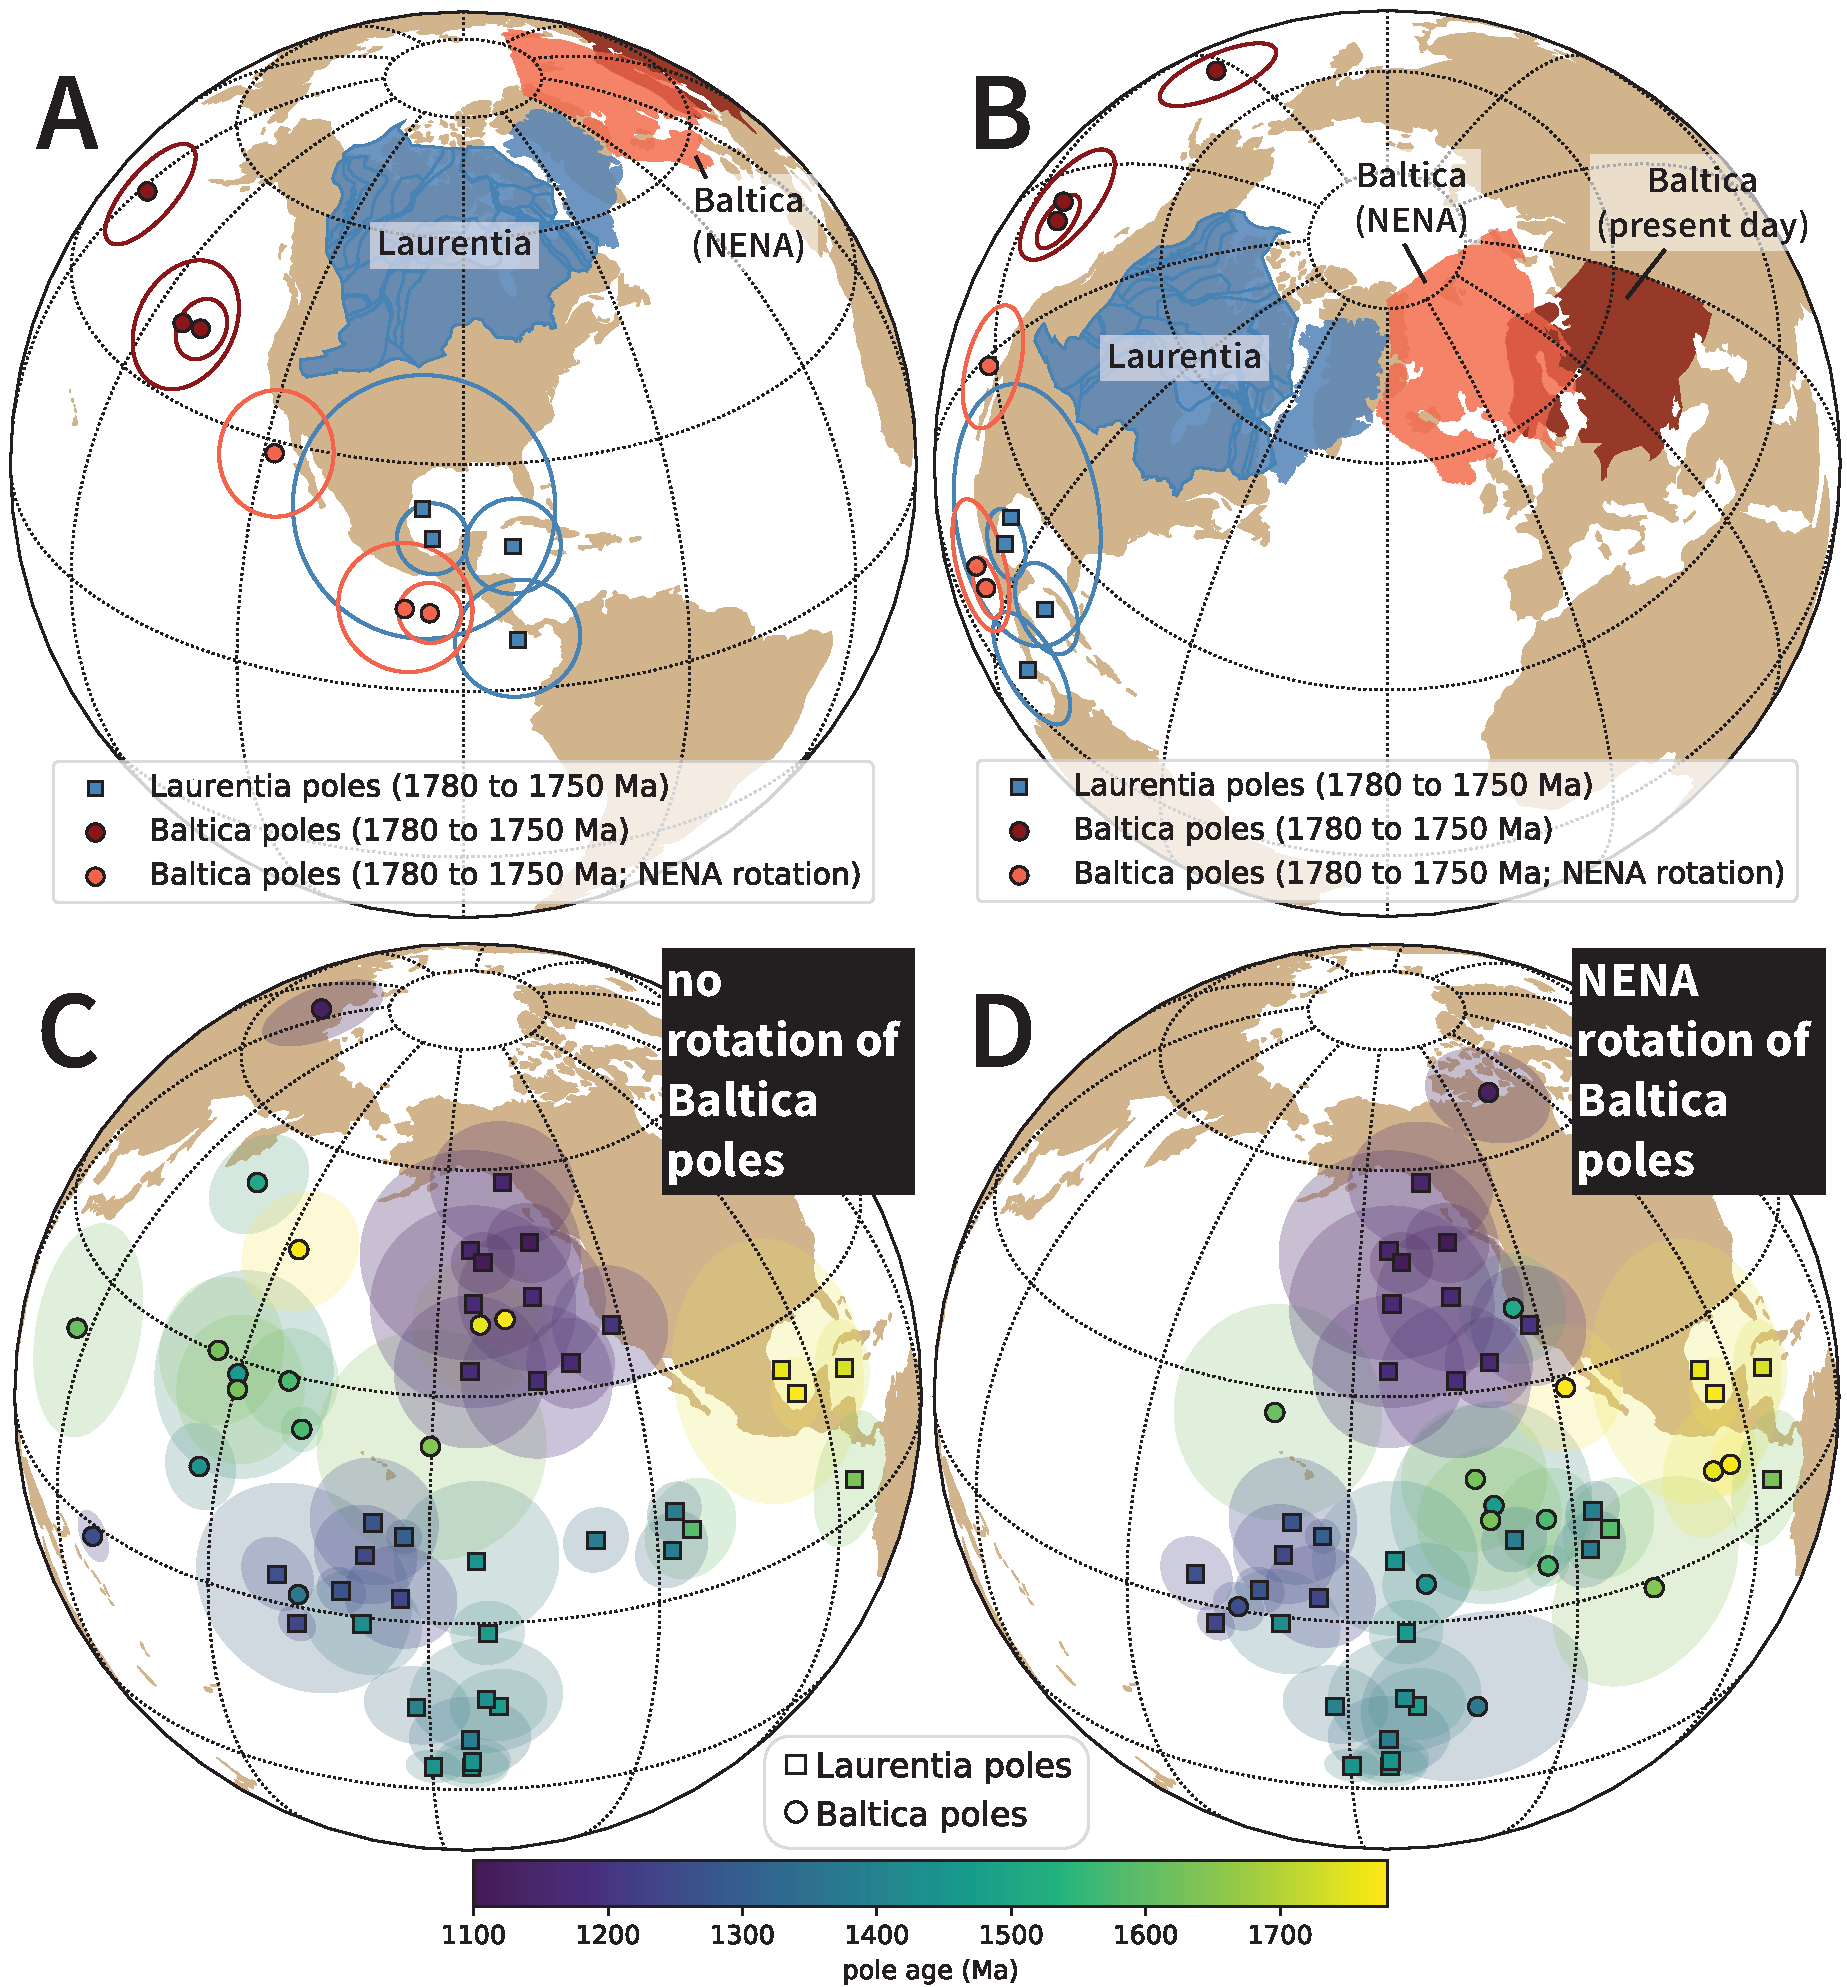
\includegraphics[width=\textwidth]{./figures/Laurentia_Baltica.pdf}
\caption{\setstretch{0.7}\small{A) Paleomagnetic poles for Laurentia and Baltica between 1780 and 1750 Ma with the Baltica poles shown with and without the NENA rotation (Euler pole for Baltica of [47.5\textdegree, 001.5\textdegree, +49.0\textdegree] as in \citeA{Evans2008a}). Baltica is shown in its present day location in dark red and shown in the NENA position in light red. B) Same data as in panel A shown with a different center of projection which allows for easier visualization of the reconstructed position. C,D) Comparison between poles between 1780 and 1110 Ma between Baltica and Laurentia without (C) and with (D) the NENA rotation. The poles that are shown are those from the Nordic compilation with 'A' and 'B' grades as well as the new ECMB pole from this study.}}
\label{fig:Laurentia_Baltica}
\end{figure}

One hypothesized connection of particular interest is that with Baltica. The two cratons have been hypothesized to have been conjoined such that they shared a margin with a long-lived history of accretionary orogenesis \cite{Hoffman1997a, Karlstrom2001a}. The proposed NENA (northern Europe and North America) configuration between Laurentia and Baltica allows for such a shared margin \cite{Gower1990a, Buchan2000a, Evans2008a}. The increased concordance between \textit{ca.} 1780 to 1750 paleomagnetic poles from Laurentia and Baltica upon the NENA rotation of Baltica can be seen in Figure \ref{fig:Laurentia_Baltica}. Paleomagnetic poles support a continued NENA connection until at least 1260 Ma (supported by poles from Baltica's \textit{ca.} 1258 Ma post-Jotnian intrusions and Laurentia's \textit{ca.} 1267 Ma Mackenzie dikes) and perhaps to 1120 Ma (where the paleomagnetic comparison is reliant on the \textit{ca.} 1122 Ma Salla dike of Baltica developed from a single cooling unit; \citeA{Salminen2009b}). This connection supports the long-lived active margin where Laurentia grew through the rest of the Paleoproterozoic and through the Mesoproterozoic until the \textit{ca.} 1.08 Ga continent-continent collision of the Grenvillian orogeny \cite{Whitmeyer2007a}.

\section{Conclusions}

The East-Central Minnesota Batholith was emplaced following Penokean orogenesis on the southeast margin of the Superior Province. While the southeast margin of Laurentia experienced subsequent intervals of accretionary orogenesis, thermochronology data constrain the batholith to have a straight-forward history of post-emplacement rapid exhumation without substantial reheating. Subsequent orogenesis occurred well southeast of the batholith --- consistent with the batholith having played a role in stabilizing Laurentian lithosphere.  Comagmatic diabase dikes of the East-Central Minnesota Batholith can be constrained through U-Pb geochronology on the felsic units to have been emplaced at 1779.1 $\pm$ 2.3 Ma. A new paleomagnetic pole developed from the magnetite remanence of these dikes provides a high-quality constraint on the position of Laurentia following Trans-Hudson orogenesis. This pole confirms the coherency of an amalgamated Laurentia at the time and supports the NENA connection with Baltica. This paleomagnetic coherency further strengthens the case that previously disparate pole positions between the Superior and Slave provinces are the result of \textit{ca.} 2.2 to 1.8 Ga mobile-lid plate tectonics. The geologic and paleomagnetic record of Laurentia is inconsistent with a stagnant-lid regime anytime over the past 2.2 billion years.

\begin{table}[h!]
\footnotesize
\caption{Summary of site level paleomagnetic data}
\begin{tabular}{lcccccccccc}
\hline
site & site lat & site lon & n & dec & inc & k & R & $\alpha_{95}$ & VGP lat & VGP lon \\
\hline
\multicolumn{11}{@{}l}{\textit{northeast-trending dike magnetite-component site means}}\\
NED1 & 45.53423 & 265.75804 &             8 &   157.6 &    74.7 &   380 &  7.98 &         2.8 &    18.4 &   276.9 \\								
  NED2 & 45.53421 & 265.75816 &             8 &   172.3 &    74.9 &   420 &  7.98 &         2.7 &    17.4 &   269.6 \\								
  NED5 & 45.53309 & 265.75803 &             6 &   170.3 &    79.0 &   213 &  5.98 &         4.6 &    24.5 &   269.6 \\								
  NED6 & 45.53299 & 265.75773 &             9 &   197.8 &    73.6 &   183 &  8.96 &         3.8 &    16.1 &   256.5 \\								
  NED7 & 45.53288 & 265.75767 &             5 &   266.3 &    81.3 &   204 &  4.98 &         5.4 &    42.0 &   242.6 \\								
  NED8 & 45.53286 & 265.75782 &             7 &   202.6 &    78.6 &   423 &  6.99 &         2.9 &    24.8 &   256.6 \\								
  NED9 & 45.53314 & 265.75855 &             7 &   191.1 &    71.5 &    90 &  6.93 &         6.4 &    12.2 &   259.5 \\								
 NED10 & 45.53259 & 265.75742 &             6 &   199.7 &    73.3 &   324 &  5.98 &         3.7 &    15.8 &   255.4 \\								
 NED11 & 45.53252 & 265.75768 &             7 &   166.1 &    75.1 &   391 &  6.98 &         3.1 &    18.1 &   272.6 \\								
 NED12 & 45.53489 & 265.76076 &             6 &   179.5 &    73.0 &   374 &  5.99 &         3.5 &    14.1 &   266.0 \\								
 NED13 & 45.53497 & 265.76113 &             7 &   169.1 &    73.9 &   199 &  6.97 &         4.3 &    15.9 &   271.4 \\								
 NED14 & 45.53492 & 265.76119 &             6 &   193.0 &    70.0 &   217 &  5.98 &         4.6 &    10.1 &   258.0 \\								
 NED15 & 45.53688 & 265.76758 &             8 &   175.8 &    77.7 &   604 &  7.99 &         2.3 &    22.0 &   267.6 \\								
 NED16 & 45.53728 & 265.76822 &             5 &   185.1 &    78.6 &   449 &  4.99 &         3.6 &    23.6 &   263.7 \\								
 NED18 & 45.53124 & 265.76945 &             6 &   134.7 &    81.7 &   159 &  5.97 &         5.3 &    33.2 &   279.5 \\								
 NED23 & 45.53398 & 265.74200 &             7 &   193.0 &    76.4 &   411 &  6.99 &         3.0 &    20.2 &   259.7 \\								
 NED25 & 45.53396 & 265.74119 &             4 &   135.4 &    80.7 &   334 &  3.99 &         5.0 &    31.5 &   280.6 \\								
 NED26 & 45.53445 & 265.74129 &             5 &   151.1 &    73.4 &   572 &  4.99 &         3.2 &    17.4 &   280.8 \\								
 NED28 & 45.53467 & 265.73817 &             4 &   157.8 &    73.8 &   145 &  3.98 &         7.7 &    16.9 &   277.2 \\								
 NED29 & 45.53438 & 265.73690 &             8 &   219.0 &    76.7 &   119 &  7.94 &         5.1 &    24.4 &   248.6 \\								
 NED31 & 45.53385 & 265.75785 &             3 &   184.7 &    69.4 &  1730 &  3.00 &         3.0 &     8.7 &   262.9 \\								
 NED34 & 45.51700 & 265.78083 &             8 &   185.9 &    77.0 &   362 &  7.98 &         2.9 &    20.8 &   263.1 \\								
 NED35 & 45.53320 & 265.75761 &             8 &   166.4 &    74.7 &   261 &  7.97 &         3.4 &    17.4 &   272.6 \\
 \multicolumn{11}{@{}l}{\textbf{mean pole: pole longitude: 265.8; pole latitude: 20.4; A$_{95}$: 4.5; K: 45.6 N: 23}}\\
\multicolumn{11}{@{}l}{\textit{northwest-trending dike magnetite-component site mean}}\\
NWD1 & 45.53407 & 265.76852 &             9 &   293.4 &    41.6 &    66 &  8.88 &         6.4 &    32.9 &   177.5 \\
\hline
\end{tabular}
\begin{tablenotes}
Notes: site lat--latitude of site (\textdegree; WGS84); site lon--longitude of site (\textdegree; WGS84) n--number of samples analyzed and included in the site mean; dec--tilt-correction mean declination for the site; inc--tilt-correction mean inclination for the site; k--Fisher precision parameter; R--resultant vector length; $\alpha_{95}$--95$\%$ confidence limit in degrees; VGP lat--latitude of the virtual geomagnetic pole for the site; VGP lon--longitude of the virtual geomagnetic pole for the site.
\end{tablenotes}
\label{tab:pmag_sites}
\end{table}

\begin{table}[h!]
\footnotesize
\caption{Summary of ID-TIMS $^{207}$Pb/$^{206}$Pb East-Central Minnesota Batholith zircon dates}
\begin{tabular}{p{1 cm}p{2.4 cm}p{1.8 cm}ccccc}
\hline
Sample & Unit & Latitude & $^{207}$Pb/$^{206}$Pb & \multicolumn{2}{c}{Uncertainty (2$\sigma$)} & MSWD & n/N \\
 &  & Longitude & date (Ma) & X & Z & & \\
\hline
ECMB6 & St. Cloud Granite & 45.53396$^{\circ}$ N 94.23187$^{\circ}$ W & 1781.44 & 0.51 & 2.4 & 1.24 & 8/8 \\
%\hline
QP1 & quartz-feldspar porphyry dike & 45.53481$^{\circ}$ N 94.25811$^{\circ}$ W & 1780.78 & 0.45 & 2.4 & 0.53 & 8/8 \\
%\hline
ECMB4 & Richmond Granite & 45.44343$^{\circ}$ N 94.48360$^{\circ}$ W & 1776.76 & 0.49 & 2.4 & 1.15 & 7/8 \\
\hline
\end{tabular}\\
%\begin{tablenotes}[para,flushleft]
Notes: X is 2$\sigma$ analytical uncertainty; Z is 2$\sigma$ uncertainty including decay constant uncertainty. This Z uncertainty needs to be utilized when comparing to dates using other decay systems (e.g., $^{40}$Ar/$^{39}$Ar, $^{187}$Re-$^{187}$Os); MSWD is the mean squared weighted deviation; n is the number of individual zircon dates included in the calculated sample mean date; N is the number of individual zircons analyzed for the sample.
%\end{tablenotes}
\label{tab:geochron}
\end{table}

% \begin{table}[h!]
% \footnotesize
% \caption{Summary of paleomagnetic poles}
% \begin{tabular}{p{3 cm}cccccccc}
% \hline
% & age (Ma) &pole & pole & A$_{95}$ &  &  &  & reference \\
% unit name & age (Ma) &lon (\textdegree) &lat (\textdegree) & A$_{95}$ & K & R & N & reference \\
% \hline
% ECMB diabase dikes \textit{southern Superior province} & 1779 $\pm$ 3 Ma & 265.8 & 23.4 &  6.2 & 26.0 & 21.2 &  22 & this study \\
% Jan Lake Granite \textit{trans-Hudson orogen} & 1758 $\pm$ 1 Ma &  &  &  &  &  &  & \citeA{Gala1995a} \\
% \hline
% Cleaver Dykes \textit{Great Bear Magmatic Arc on margin of Slave Province} & 17XX $\pm$ 1 Ma &  &  &  &  &  &  & \citeA{Gala1995a} \\
% \hline
% \end{tabular}
% \begin{tablenotes}
% Notes: pole lon--longitude of paleomagnetic pole; pole lat--latitude of paleomagnetic pole; A$_{95}$--confidence limit of pole mean degrees; K--Fisher precision parameter; R--resultant vector length; N--number of dike site mean virtual geomagnetic poles used to calculate the mean pole.
% \end{tablenotes}
% \label{tab:poles}
% \end{table}

%Text here ===>>>

%%

%  Numbered lines in equations:
%  To add line numbers to lines in equations,
%  \begin{linenomath*}
%  \begin{equation}
%  \end{equation}
%  \end{linenomath*}



%% Enter Figures and Tables near as possible to where they are first mentioned:
%
% DO NOT USE \psfrag or \subfigure commands.
%
% Figure captions go below the figure.
% Table titles go above tables;  other caption information
%  should be placed in last line of the table, using
% \multicolumn2l{$^a$ This is a table note.}
%
%----------------
% EXAMPLE FIGURE
%
% \begin{figure}[h]
% \centering
% when using pdflatex, use pdf file:
% \includegraphics[natwidth=800px,natheight=600px]{figsamp.pdf}
%
% when using dvips, use .eps file:
% \includegraphics[natwidth=800px,natheight=600px]{figsamp.eps}
%
% \caption{Short caption}
% \label{figone}
%  \end{figure}
%
% We recommend that you provide the native width and height (natwidth, natheight) of your figures.
% Specifying native dimensions ensures that your figures are properly scaled
%
%
% ---------------
% EXAMPLE TABLE
%
% \begin{table}
% \caption{Time of the Transition Between Phase 1 and Phase 2$^{a}$}
% \centering
% \begin{tabular}{l c}
% \hline
%  Run  & Time (min)  \\
% \hline
%   $l1$  & 260   \\
%   $l2$  & 300   \\
%   $l3$  & 340   \\
%   $h1$  & 270   \\
%   $h2$  & 250   \\
%   $h3$  & 380   \\
%   $r1$  & 370   \\
%   $r2$  & 390   \\
% \hline
% \multicolumn{2}{l}{$^{a}$Footnote text here.}
% \end{tabular}
% \end{table}

%% SIDEWAYS FIGURE and TABLE
% AGU prefers the use of {sidewaystable} over {landscapetable} as it causes fewer problems.
%
% \begin{sidewaysfigure}
% \includegraphics[width=20pc]{figsamp}
% \caption{caption here}
% \label{newfig}
% \end{sidewaysfigure}
%
%  \begin{sidewaystable}
%  \caption{Caption here}
% \label{tab:signif_gap_clos}
%  \begin{tabular}{ccc}
% one&two&three\\
% four&five&six
%  \end{tabular}
%  \end{sidewaystable}

%% If using numbered lines, please surround equations with \begin{linenomath*}...\end{linenomath*}
%\begin{linenomath*}
%\begin{equation}
%y|{f} \sim g(m, \sigma),
%\end{equation}
%\end{linenomath*}

%%% End of body of article

%%%%%%%%%%%%%%%%%%%%%%%%%%%%%%%%%%%%%%%%%%%%%%%%%%%%%%%%%%%%%%%%
%
%  ACKNOWLEDGMENTS
%
% The acknowledgments must list:
%
% >>>>	A statement that indicates to the reader where the data
% 	supporting the conclusions can be obtained (for example, in the
% 	references, tables, supporting information, and other databases).
%
% 	All funding sources related to this work from all authors
%
% 	Any real or perceived financial conflicts of interests for any
%	author
%
% 	Other affiliations for any author that may be perceived as
% 	having a conflict of interest with respect to the results of this
% 	paper.
%
%
% It is also the appropriate place to thank colleagues and other contributors.
% AGU does not normally allow dedications.


\acknowledgments
This research was supported by the National Science Foundation through CAREER grant EAR-1847277 awarded to N.L.S.-H.. Rock magnetic experiments using the MPMS were conducted at the Institute for Rock Magnetism which is supported by the Instrumentation and Facilities program of the National Science Foundation, Earth Science Division. We gratefully acknowledge Mark Schmitz and Jim Crowley for analytical support at the Boise State Isotope Geology Laboratory. Noah McLean provided insight for the methodology applied to interpret the uncertainty associated with the age of a unit bracketed by U-Pb dates. We thank Stearns County Parks for research permits that enabled sample collection in Quarry Park and Nature Preserve. The manuscript was improved through thoughtful reviews from Daniel Holm, Anthony Pivarunas, and an anonymous reviewer. Paleomagnetic data associated with this study are available within the MagIC database (\url{https://earthref.org/MagIC/17072/162b766f-435a-4053-bf63-0a5246c24339}; UPDATE TO DOI WHEN ASSIGNED) and all data are within a Github repository associated with this work (\url{https://github.com/Swanson-Hysell-Group/2021_ECMB}) that is also archived on Zenodo (https://doi.org/10.5281/zenodo.4625041). This repository also contains Python code related to calculations, visualizations and statistical tests discussed herein.  

%% ------------------------------------------------------------------------ %%
%% References and Citations

%%%%%%%%%%%%%%%%%%%%%%%%%%%%%%%%%%%%%%%%%%%%%%%
% BibTeX is preferred:
%
%\bibliography{../../references/allrefs}
%
\begin{thebibliography}{}

\bibitem [\protect \citeauthoryear {%
Ague%
}{%
Ague%
}{%
{\protect \APACyear {1997}}%
}]{%
Ague1997a}
\APACinsertmetastar {%
Ague1997a}%
\begin{APACrefauthors}%
Ague, J\BPBI J.%
\end{APACrefauthors}%
\unskip\
\newblock
\APACrefYearMonthDay{1997}{}{}.
\newblock
{\BBOQ}\APACrefatitle {Thermodynamic calculation of emplacement pressures for
  batholithic rocks, {C}alifornia: Implications for the aluminum-in-hornblende
  barometer} {Thermodynamic calculation of emplacement pressures for
  batholithic rocks, {C}alifornia: Implications for the aluminum-in-hornblende
  barometer}.{\BBCQ}
\newblock
\APACjournalVolNumPages{Geology}{25}{6}{563}.
\newblock
\begin{APACrefDOI} \doi{10.1130/0091-7613(1997)025<0563:tcoepf>2.3.co;2}
  \end{APACrefDOI}
\PrintBackRefs{\CurrentBib}

\bibitem [\protect \citeauthoryear {%
Besnus%
\ \BBA {} Meyer%
}{%
Besnus%
\ \BBA {} Meyer%
}{%
{\protect \APACyear {1964}}%
}]{%
Besnus1964a}
\APACinsertmetastar {%
Besnus1964a}%
\begin{APACrefauthors}%
Besnus, M\BPBI J.%
\BCBT {}\ \BBA {} Meyer, A\BPBI J.%
\end{APACrefauthors}%
\unskip\
\newblock
\APACrefYearMonthDay{1964}{}{}.
\newblock
{\BBOQ}\APACrefatitle {Nouvelles donn{\'e}es exp{\'e}rimentales sur le
  magn{\'e}tisme de la pyrrhotine naturelle} {Nouvelles donn{\'e}es
  exp{\'e}rimentales sur le magn{\'e}tisme de la pyrrhotine naturelle}.{\BBCQ}
\newblock
\BIn{} \APACrefbtitle {Proc. Int. Conf. Mag.} {Proc. int. conf. mag.}\
  (\BVOL~20, \BPG~507-511).
\PrintBackRefs{\CurrentBib}

\bibitem [\protect \citeauthoryear {%
Bickford%
, Mock%
, Steinhart~III%
, Collerson%
\BCBL {}\ \BBA {} Lewry%
}{%
Bickford%
\ \protect \BOthers {.}}{%
{\protect \APACyear {2005}}%
}]{%
Bickford2005a}
\APACinsertmetastar {%
Bickford2005a}%
\begin{APACrefauthors}%
Bickford, M\BPBI E.%
, Mock, T\BPBI D.%
, Steinhart~III, W\BPBI E.%
, Collerson, K\BPBI D.%
\BCBL {}\ \BBA {} Lewry, J\BPBI F.%
\end{APACrefauthors}%
\unskip\
\newblock
\APACrefYearMonthDay{2005}{}{}.
\newblock
{\BBOQ}\APACrefatitle {{Origin of the Archean Sask craton and its extent within
  the Trans-Hudson orogen: evidence from Pb and Nd isotopic compositions of
  basement rocks and post-orogenic intrusions}} {{Origin of the Archean Sask
  craton and its extent within the Trans-Hudson orogen: evidence from Pb and Nd
  isotopic compositions of basement rocks and post-orogenic
  intrusions}}.{\BBCQ}
\newblock
\APACjournalVolNumPages{Canadian Journal of Earth Sciences}{42}{}{659--684}.
\newblock
\begin{APACrefDOI} \doi{10.1139/e04-064} \end{APACrefDOI}
\PrintBackRefs{\CurrentBib}

\bibitem [\protect \citeauthoryear {%
Bispo-Santos%
, D'Agrella-Filho%
, Trindade%
, Janikian%
\BCBL {}\ \BBA {} Reis%
}{%
Bispo-Santos%
\ \protect \BOthers {.}}{%
{\protect \APACyear {2014}}%
}]{%
Bispo-Santos2014a}
\APACinsertmetastar {%
Bispo-Santos2014a}%
\begin{APACrefauthors}%
Bispo-Santos, F.%
, D'Agrella-Filho, M\BPBI S.%
, Trindade, R\BPBI I.%
, Janikian, L.%
\BCBL {}\ \BBA {} Reis, N\BPBI J.%
\end{APACrefauthors}%
\unskip\
\newblock
\APACrefYearMonthDay{2014}{}{}.
\newblock
{\BBOQ}\APACrefatitle {{Was there SAMBA in Columbia? Paleomagnetic evidence
  from 1790 Ma Avanavero mafic sills (northern Amazonian Craton)}} {{Was there
  SAMBA in Columbia? Paleomagnetic evidence from 1790 Ma Avanavero mafic sills
  (northern Amazonian Craton)}}.{\BBCQ}
\newblock
\APACjournalVolNumPages{Precambrian Research}{244}{}{139--155}.
\newblock
\begin{APACrefDOI} \doi{10.1016/j.precamres.2013.11.002} \end{APACrefDOI}
\PrintBackRefs{\CurrentBib}

\bibitem [\protect \citeauthoryear {%
Boerboom%
\ \BBA {} Holm%
}{%
Boerboom%
\ \BBA {} Holm%
}{%
{\protect \APACyear {2000}}%
}]{%
Boerboom2000a}
\APACinsertmetastar {%
Boerboom2000a}%
\begin{APACrefauthors}%
Boerboom, T\BPBI J.%
\BCBT {}\ \BBA {} Holm, D\BPBI K.%
\end{APACrefauthors}%
\unskip\
\newblock
\APACrefYearMonthDay{2000}{}{}.
\newblock
{\BBOQ}\APACrefatitle {{Paleoproterozoic Intrusive Igneous Rocks of
  Southeastern Stearns County, Central Minnesota}} {{Paleoproterozoic Intrusive
  Igneous Rocks of Southeastern Stearns County, Central Minnesota}}.{\BBCQ}
\newblock
\APACjournalVolNumPages{Minnesota Geological Survey Report of Investigations
  56}{}{}{}.
\PrintBackRefs{\CurrentBib}

\bibitem [\protect \citeauthoryear {%
Boerboom%
, Holm%
\BCBL {}\ \BBA {} Van~Schmus%
}{%
Boerboom%
\ \protect \BOthers {.}}{%
{\protect \APACyear {2011}}%
}]{%
Boerboom2011b}
\APACinsertmetastar {%
Boerboom2011b}%
\begin{APACrefauthors}%
Boerboom, T\BPBI J.%
, Holm, D\BPBI K.%
\BCBL {}\ \BBA {} Van~Schmus, R.%
\end{APACrefauthors}%
\unskip\
\newblock
\APACrefYearMonthDay{2011}{}{}.
\newblock
{\BBOQ}\APACrefatitle {{Late Paleoproterozoic deformational, metamorphic, and
  magmatic history of east-central Minnesota}} {{Late Paleoproterozoic
  deformational, metamorphic, and magmatic history of east-central
  Minnesota}}.{\BBCQ}
\newblock
\APACjournalVolNumPages{Archean to Anthropocene: Field Guides to the Geology of
  the Mid-Continent of North America}{}{}{1--23}.
\newblock
\begin{APACrefDOI} \doi{10.1130/2011.0024(01)} \end{APACrefDOI}
\PrintBackRefs{\CurrentBib}

\bibitem [\protect \citeauthoryear {%
Boerboom%
, Holm%
\BCBL {}\ \BBA {} Van~Schmus%
}{%
Boerboom%
\ \protect \BOthers {.}}{%
{\protect \APACyear {2005}}%
}]{%
Boerboom2005b}
\APACinsertmetastar {%
Boerboom2005b}%
\begin{APACrefauthors}%
Boerboom, T\BPBI J.%
, Holm, D\BPBI K.%
\BCBL {}\ \BBA {} Van~Schmus, W\BPBI R.%
\end{APACrefauthors}%
\unskip\
\newblock
\APACrefYearMonthDay{2005}{}{}.
\newblock
{\BBOQ}\APACrefatitle {{Granites of the East-Central Minnesota Batholith}}
  {{Granites of the East-Central Minnesota Batholith}}.{\BBCQ}
\newblock
\APACjournalVolNumPages{Minnesota Geological Survey Guidebook}{}{}{}.
\PrintBackRefs{\CurrentBib}

\bibitem [\protect \citeauthoryear {%
Boerboom%
, Setterholm%
\BCBL {}\ \BBA {} Chandler%
}{%
Boerboom%
\ \protect \BOthers {.}}{%
{\protect \APACyear {1995}}%
}]{%
Boerboom1995a}
\APACinsertmetastar {%
Boerboom1995a}%
\begin{APACrefauthors}%
Boerboom, T\BPBI J.%
, Setterholm, D\BPBI R.%
\BCBL {}\ \BBA {} Chandler, V\BPBI W.%
\end{APACrefauthors}%
\unskip\
\newblock
\APACrefYearMonthDay{1995}{}{}.
\newblock
{\BBOQ}\APACrefatitle {Bedrock geology pl. 2} {Bedrock geology pl. 2}.{\BBCQ}
\newblock
\BIn{} G\BPBI N.~Meyer\ (\BED), \APACrefbtitle {{Geologic atlas of Stearns
  County, Minnesota: Minnesota Geological Survey County Atlas C-10, pt. A., 7
  pls., scales 1:100,000 and 1:200,000}.} {{Geologic atlas of Stearns County,
  Minnesota: Minnesota Geological Survey County Atlas C-10, pt. A., 7 pls.,
  scales 1:100,000 and 1:200,000}.}
\newblock
\APACaddressPublisher{}{Minnesota Geological Survey}.
\PrintBackRefs{\CurrentBib}

\bibitem [\protect \citeauthoryear {%
Buchan%
\ \protect \BOthers {.}}{%
Buchan%
\ \protect \BOthers {.}}{%
{\protect \APACyear {2000}}%
}]{%
Buchan2000a}
\APACinsertmetastar {%
Buchan2000a}%
\begin{APACrefauthors}%
Buchan, K\BPBI L.%
, Mertanen, S.%
, Park, R.%
, Pesonen, L.%
, Elming, S\BPBI A.%
, Abrahamsen, N.%
\BCBL {}\ \BBA {} Bylund, G.%
\end{APACrefauthors}%
\unskip\
\newblock
\APACrefYearMonthDay{2000}{}{}.
\newblock
{\BBOQ}\APACrefatitle {Comparing the drift of {L}aurentia and {B}altica in the
  {P}roterozoic: the importance of key paleomagnetic poles} {Comparing the
  drift of {L}aurentia and {B}altica in the {P}roterozoic: the importance of
  key paleomagnetic poles}.{\BBCQ}
\newblock
\APACjournalVolNumPages{Tectonophysics}{319}{}{167-198}.
\newblock
\begin{APACrefDOI} \doi{10.1016/S0040-1951(00)00032-9} \end{APACrefDOI}
\PrintBackRefs{\CurrentBib}

\bibitem [\protect \citeauthoryear {%
Buchan%
, Mitchell%
, Bleeker%
, Hamilton%
\BCBL {}\ \BBA {} LeCheminant%
}{%
Buchan%
\ \protect \BOthers {.}}{%
{\protect \APACyear {2016}}%
}]{%
Buchan2016a}
\APACinsertmetastar {%
Buchan2016a}%
\begin{APACrefauthors}%
Buchan, K\BPBI L.%
, Mitchell, R\BPBI N.%
, Bleeker, W.%
, Hamilton, M\BPBI A.%
\BCBL {}\ \BBA {} LeCheminant, A\BPBI N.%
\end{APACrefauthors}%
\unskip\
\newblock
\APACrefYearMonthDay{2016}{}{}.
\newblock
{\BBOQ}\APACrefatitle {{Paleomagnetism of ca. 2.13--2.11 Ga Indin and ca. 1.885
  Ga Ghost dyke swarms of the Slave craton: Implications for the Slave craton
  APW path and relative drift of Slave, Superior and Siberian cratons in the
  Paleoproterozoic}} {{Paleomagnetism of ca. 2.13--2.11 Ga Indin and ca. 1.885
  Ga Ghost dyke swarms of the Slave craton: Implications for the Slave craton
  APW path and relative drift of Slave, Superior and Siberian cratons in the
  Paleoproterozoic}}.{\BBCQ}
\newblock
\APACjournalVolNumPages{Precambrian Research}{275}{}{151--175}.
\newblock
\begin{APACrefDOI} \doi{10.1016/j.precamres.2016.01.012} \end{APACrefDOI}
\PrintBackRefs{\CurrentBib}

\bibitem [\protect \citeauthoryear {%
Chamberlain%
\ \BBA {} Bowring%
}{%
Chamberlain%
\ \BBA {} Bowring%
}{%
{\protect \APACyear {2001}}%
}]{%
Chamberlain2001a}
\APACinsertmetastar {%
Chamberlain2001a}%
\begin{APACrefauthors}%
Chamberlain, K\BPBI R.%
\BCBT {}\ \BBA {} Bowring, S\BPBI A.%
\end{APACrefauthors}%
\unskip\
\newblock
\APACrefYearMonthDay{2001}{}{}.
\newblock
{\BBOQ}\APACrefatitle {Apatite--feldspar {U}--{P}b thermochronometer: a
  reliable, mid-range ($\sim$450{\textdegree}{C}), diffusion-controlled system}
  {Apatite--feldspar {U}--{P}b thermochronometer: a reliable, mid-range
  ($\sim$450{\textdegree}{C}), diffusion-controlled system}.{\BBCQ}
\newblock
\APACjournalVolNumPages{Chemical Geology}{172}{1-2}{173--200}.
\newblock
\begin{APACrefDOI} \doi{10.1016/s0009-2541(00)00242-4} \end{APACrefDOI}
\PrintBackRefs{\CurrentBib}

\bibitem [\protect \citeauthoryear {%
Cherniak%
, Lanford%
\BCBL {}\ \BBA {} Ryerson%
}{%
Cherniak%
\ \protect \BOthers {.}}{%
{\protect \APACyear {1991}}%
}]{%
Cherniak1991a}
\APACinsertmetastar {%
Cherniak1991a}%
\begin{APACrefauthors}%
Cherniak, D.%
, Lanford, W.%
\BCBL {}\ \BBA {} Ryerson, F.%
\end{APACrefauthors}%
\unskip\
\newblock
\APACrefYearMonthDay{1991}{}{}.
\newblock
{\BBOQ}\APACrefatitle {Lead diffusion in apatite and zircon using ion
  implantation and {R}utherford Backscattering techniques} {Lead diffusion in
  apatite and zircon using ion implantation and {R}utherford backscattering
  techniques}.{\BBCQ}
\newblock
\APACjournalVolNumPages{Geochimica et Cosmochimica Acta}{55}{6}{1663--1673}.
\newblock
\begin{APACrefDOI} \doi{10.1016/0016-7037(91)90137-t} \end{APACrefDOI}
\PrintBackRefs{\CurrentBib}

\bibitem [\protect \citeauthoryear {%
Cherniak%
\ \BBA {} Watson%
}{%
Cherniak%
\ \BBA {} Watson%
}{%
{\protect \APACyear {2001}}%
}]{%
Cherniak2001a}
\APACinsertmetastar {%
Cherniak2001a}%
\begin{APACrefauthors}%
Cherniak, D.%
\BCBT {}\ \BBA {} Watson, E.%
\end{APACrefauthors}%
\unskip\
\newblock
\APACrefYearMonthDay{2001}{}{}.
\newblock
{\BBOQ}\APACrefatitle {Pb diffusion in zircon} {Pb diffusion in zircon}.{\BBCQ}
\newblock
\APACjournalVolNumPages{Chemical Geology}{172}{1-2}{5--24}.
\newblock
\begin{APACrefDOI} \doi{10.1016/s0009-2541(00)00233-3} \end{APACrefDOI}
\PrintBackRefs{\CurrentBib}

\bibitem [\protect \citeauthoryear {%
Cochrane%
\ \protect \BOthers {.}}{%
Cochrane%
\ \protect \BOthers {.}}{%
{\protect \APACyear {2014}}%
}]{%
Cochrane2014a}
\APACinsertmetastar {%
Cochrane2014a}%
\begin{APACrefauthors}%
Cochrane, R.%
, Spikings, R\BPBI A.%
, Chew, D.%
, Wotzlaw, J\BHBI F.%
, Chiaradia, M.%
, Tyrrell, S.%
\BDBL {}der Lelij, R\BPBI V.%
\end{APACrefauthors}%
\unskip\
\newblock
\APACrefYearMonthDay{2014}{}{}.
\newblock
{\BBOQ}\APACrefatitle {High temperature ($>$350{\textdegree}{C})
  thermochronology and mechanisms of {P}b loss in apatite} {High temperature
  ($>$350{\textdegree}{C}) thermochronology and mechanisms of {P}b loss in
  apatite}.{\BBCQ}
\newblock
\APACjournalVolNumPages{Geochimica et Cosmochimica Acta}{127}{}{39--56}.
\newblock
\begin{APACrefDOI} \doi{10.1016/j.gca.2013.11.028} \end{APACrefDOI}
\PrintBackRefs{\CurrentBib}

\bibitem [\protect \citeauthoryear {%
Corrigan%
, Pehrsson%
, Wodicka%
\BCBL {}\ \BBA {} de Kemp%
}{%
Corrigan%
\ \protect \BOthers {.}}{%
{\protect \APACyear {2009}}%
}]{%
Corrigan2009a}
\APACinsertmetastar {%
Corrigan2009a}%
\begin{APACrefauthors}%
Corrigan, D.%
, Pehrsson, S.%
, Wodicka, N.%
\BCBL {}\ \BBA {} de Kemp, E.%
\end{APACrefauthors}%
\unskip\
\newblock
\APACrefYearMonthDay{2009}{}{}.
\newblock
{\BBOQ}\APACrefatitle {{The Palaeoproterozoic Trans-Hudson Orogen: a prototype
  of modern accretionary processes}} {{The Palaeoproterozoic Trans-Hudson
  Orogen: a prototype of modern accretionary processes}}.{\BBCQ}
\newblock
\APACjournalVolNumPages{Geological Society, London, Special
  Publications}{327}{1}{457--479}.
\newblock
\begin{APACrefDOI} \doi{10.1144/sp327.19} \end{APACrefDOI}
\PrintBackRefs{\CurrentBib}

\bibitem [\protect \citeauthoryear {%
D'Agrella-Filho%
, Teixeira%
, da Trindade%
, Patroni%
\BCBL {}\ \BBA {} Prieto%
}{%
D'Agrella-Filho%
\ \protect \BOthers {.}}{%
{\protect \APACyear {2020}}%
}]{%
DAgrella-Filho2020a}
\APACinsertmetastar {%
DAgrella-Filho2020a}%
\begin{APACrefauthors}%
D'Agrella-Filho, M\BPBI S.%
, Teixeira, W.%
, da Trindade, R\BPBI I.%
, Patroni, O\BPBI A.%
\BCBL {}\ \BBA {} Prieto, R\BPBI F.%
\end{APACrefauthors}%
\unskip\
\newblock
\APACrefYearMonthDay{2020}{}{}.
\newblock
{\BBOQ}\APACrefatitle {{Paleomagnetism of 1.79 Ga Par{\'a} de Minas mafic
  dykes: Testing a S{\~a}o Francisco/Congo-North China-Rio de la Plata
  connection in Columbia}} {{Paleomagnetism of 1.79 Ga Par{\'a} de Minas mafic
  dykes: Testing a S{\~a}o Francisco/Congo-North China-Rio de la Plata
  connection in Columbia}}.{\BBCQ}
\newblock
\APACjournalVolNumPages{Precambrian Research}{338}{}{105584}.
\newblock
\begin{APACrefDOI} \doi{10.1016/j.precamres.2019.105584} \end{APACrefDOI}
\PrintBackRefs{\CurrentBib}

\bibitem [\protect \citeauthoryear {%
Deenen%
, Langereis%
, van Hinsbergen%
\BCBL {}\ \BBA {} Biggin%
}{%
Deenen%
\ \protect \BOthers {.}}{%
{\protect \APACyear {2011}}%
}]{%
Deenen2011a}
\APACinsertmetastar {%
Deenen2011a}%
\begin{APACrefauthors}%
Deenen, M\BPBI H\BPBI L.%
, Langereis, C\BPBI G.%
, van Hinsbergen, D\BPBI J\BPBI J.%
\BCBL {}\ \BBA {} Biggin, A\BPBI J.%
\end{APACrefauthors}%
\unskip\
\newblock
\APACrefYearMonthDay{2011}{}{}.
\newblock
{\BBOQ}\APACrefatitle {Geomagnetic secular variation and the statistics of
  palaeomagnetic directions} {Geomagnetic secular variation and the statistics
  of palaeomagnetic directions}.{\BBCQ}
\newblock
\APACjournalVolNumPages{Geophysical Journal International}{}{}{}.
\newblock
\begin{APACrefDOI} \doi{10.1111/j.1365-246X.2011.05050.x} \end{APACrefDOI}
\PrintBackRefs{\CurrentBib}

\bibitem [\protect \citeauthoryear {%
Dewane%
\ \BBA {} Van~Schmus%
}{%
Dewane%
\ \BBA {} Van~Schmus%
}{%
{\protect \APACyear {2007}}%
}]{%
Dewane2007a}
\APACinsertmetastar {%
Dewane2007a}%
\begin{APACrefauthors}%
Dewane, T.%
\BCBT {}\ \BBA {} Van~Schmus, W.%
\end{APACrefauthors}%
\unskip\
\newblock
\APACrefYearMonthDay{2007}{}{}.
\newblock
{\BBOQ}\APACrefatitle {{U--Pb geochronology of the Wolf River batholith,
  north-central Wisconsin: Evidence for successive magmatism between 1484 Ma
  and 1468 Ma}} {{U--Pb geochronology of the Wolf River batholith,
  north-central Wisconsin: Evidence for successive magmatism between 1484 Ma
  and 1468 Ma}}.{\BBCQ}
\newblock
\APACjournalVolNumPages{Precambrian Research}{157}{1-4}{215--234}.
\newblock
\begin{APACrefDOI} \doi{10.1016/j.precamres.2007.02.018} \end{APACrefDOI}
\PrintBackRefs{\CurrentBib}

\bibitem [\protect \citeauthoryear {%
Dodson%
}{%
Dodson%
}{%
{\protect \APACyear {1973}}%
}]{%
Dodson1973a}
\APACinsertmetastar {%
Dodson1973a}%
\begin{APACrefauthors}%
Dodson, M\BPBI H.%
\end{APACrefauthors}%
\unskip\
\newblock
\APACrefYearMonthDay{1973}{}{}.
\newblock
{\BBOQ}\APACrefatitle {Closure temperature in cooling geochronological and
  petrological systems} {Closure temperature in cooling geochronological and
  petrological systems}.{\BBCQ}
\newblock
\APACjournalVolNumPages{Contributions to Mineralogy and
  Petrology}{40}{3}{259--274}.
\newblock
\begin{APACrefDOI} \doi{10.1007/bf00373790} \end{APACrefDOI}
\PrintBackRefs{\CurrentBib}

\bibitem [\protect \citeauthoryear {%
Evans%
, Li%
\BCBL {}\ \BBA {} Murphy%
}{%
Evans%
\ \protect \BOthers {.}}{%
{\protect \APACyear {2016}}%
}]{%
Evans2016a}
\APACinsertmetastar {%
Evans2016a}%
\begin{APACrefauthors}%
Evans, D\BPBI A\BPBI D.%
, Li, Z\BPBI X.%
\BCBL {}\ \BBA {} Murphy, J\BPBI B.%
\end{APACrefauthors}%
\unskip\
\newblock
\APACrefYearMonthDay{2016}{}{}.
\newblock
{\BBOQ}\APACrefatitle {Four-dimensional context of {E}arth's supercontinents}
  {Four-dimensional context of {E}arth's supercontinents}.{\BBCQ}
\newblock
\BIn{} D\BPBI A\BPBI D.~Evans, Z\BPBI X.~Li\BCBL {}\ \BBA {} J\BPBI B.~Murphy\
  (\BEDS), \APACrefbtitle {Supercontinent Cycles Through Earth History}
  {Supercontinent cycles through earth history}\ (\BVOL~424).
\newblock
\APACaddressPublisher{}{Geological Society, London, Special Publications}.
\newblock
\begin{APACrefDOI} \doi{10.1144/SP424.12} \end{APACrefDOI}
\PrintBackRefs{\CurrentBib}

\bibitem [\protect \citeauthoryear {%
Evans%
\ \BBA {} Mitchell%
}{%
Evans%
\ \BBA {} Mitchell%
}{%
{\protect \APACyear {2011}}%
}]{%
Evans2011a}
\APACinsertmetastar {%
Evans2011a}%
\begin{APACrefauthors}%
Evans, D\BPBI A\BPBI D.%
\BCBT {}\ \BBA {} Mitchell, R\BPBI N.%
\end{APACrefauthors}%
\unskip\
\newblock
\APACrefYearMonthDay{2011}{}{}.
\newblock
{\BBOQ}\APACrefatitle {Assembly and breakup of the core of
  {P}aleoproterozoic--{M}esoproterozoic supercontinent {N}una} {Assembly and
  breakup of the core of {P}aleoproterozoic--{M}esoproterozoic supercontinent
  {N}una}.{\BBCQ}
\newblock
\APACjournalVolNumPages{Geology}{39}{}{443-446}.
\newblock
\begin{APACrefDOI} \doi{10.1130/G31654.1} \end{APACrefDOI}
\PrintBackRefs{\CurrentBib}

\bibitem [\protect \citeauthoryear {%
Evans%
\ \protect \BOthers {.}}{%
Evans%
\ \protect \BOthers {.}}{%
{\protect \APACyear {2021}}%
}]{%
Evans2021a}
\APACinsertmetastar {%
Evans2021a}%
\begin{APACrefauthors}%
Evans, D\BPBI A\BPBI D.%
, Pesonen, L\BPBI J.%
, Eglington, B\BPBI M.%
, Elming, S\BHBI {\AA}.%
, Gong, Z.%
, Li, Z\BHBI X.%
\BDBL {}Zhang, S.%
\end{APACrefauthors}%
\unskip\
\newblock
\APACrefYearMonthDay{2021}{}{}.
\newblock
{\BBOQ}\APACrefatitle {An expanding list of reliable paleomagnetic poles for
  {P}recambrian tectonic reconstructions} {An expanding list of reliable
  paleomagnetic poles for {P}recambrian tectonic reconstructions}.{\BBCQ}
\newblock
\BIn{} L\BPBI J.~Pesonen, D\BPBI A\BPBI D.~Evans, S\BPBI {\AA}.~Elming, J\BPBI
  M.~Salminen\BCBL {}\ \BBA {} T.~Veikkolainen\ (\BEDS), \APACrefbtitle
  {Ancient Supercontinents and the Paleogeography of the Earth.} {Ancient
  supercontinents and the paleogeography of the earth.}
\newblock
\APACaddressPublisher{}{Elsevier}.
\PrintBackRefs{\CurrentBib}

\bibitem [\protect \citeauthoryear {%
Evans%
\ \BBA {} Pisarevsky%
}{%
Evans%
\ \BBA {} Pisarevsky%
}{%
{\protect \APACyear {2008}}%
}]{%
Evans2008a}
\APACinsertmetastar {%
Evans2008a}%
\begin{APACrefauthors}%
Evans, D\BPBI A\BPBI D.%
\BCBT {}\ \BBA {} Pisarevsky, S\BPBI A.%
\end{APACrefauthors}%
\unskip\
\newblock
\APACrefYearMonthDay{2008}{}{}.
\newblock
{\BBOQ}\APACrefatitle {Plate tectonics on early {E}arth? Weighing the
  paleomagnetic evidence} {Plate tectonics on early {E}arth? weighing the
  paleomagnetic evidence}.{\BBCQ}
\newblock
\APACjournalVolNumPages{Geological Society of America Special
  Papers}{440}{}{249--263}.
\newblock
\begin{APACrefDOI} \doi{10.1130/2008.2440(12)} \end{APACrefDOI}
\PrintBackRefs{\CurrentBib}

\bibitem [\protect \citeauthoryear {%
Fairchild%
, Swanson-Hysell%
, Ramezani%
, Sprain%
\BCBL {}\ \BBA {} Bowring%
}{%
Fairchild%
\ \protect \BOthers {.}}{%
{\protect \APACyear {2017}}%
}]{%
Fairchild2017a}
\APACinsertmetastar {%
Fairchild2017a}%
\begin{APACrefauthors}%
Fairchild, L\BPBI M.%
, Swanson-Hysell, N\BPBI L.%
, Ramezani, J.%
, Sprain, C\BPBI J.%
\BCBL {}\ \BBA {} Bowring, S\BPBI A.%
\end{APACrefauthors}%
\unskip\
\newblock
\APACrefYearMonthDay{2017}{}{}.
\newblock
{\BBOQ}\APACrefatitle {{The end of Midcontinent Rift magmatism and the
  paleogeography of Laurentia}} {{The end of Midcontinent Rift magmatism and
  the paleogeography of Laurentia}}.{\BBCQ}
\newblock
\APACjournalVolNumPages{Lithosphere}{9}{1}{117-133}.
\newblock
\begin{APACrefDOI} \doi{10.1130/L580.1} \end{APACrefDOI}
\PrintBackRefs{\CurrentBib}

\bibitem [\protect \citeauthoryear {%
Feinberg%
, Solheid%
, Swanson-Hysell%
, Jackson%
\BCBL {}\ \BBA {} Bowles%
}{%
Feinberg%
\ \protect \BOthers {.}}{%
{\protect \APACyear {2015}}%
}]{%
Feinberg2015a}
\APACinsertmetastar {%
Feinberg2015a}%
\begin{APACrefauthors}%
Feinberg, J.%
, Solheid, P.%
, Swanson-Hysell, N.%
, Jackson, M.%
\BCBL {}\ \BBA {} Bowles, J.%
\end{APACrefauthors}%
\unskip\
\newblock
\APACrefYearMonthDay{2015}{}{}.
\newblock
{\BBOQ}\APACrefatitle {Full vector low-temperature magnetic measurements of
  geologic materials} {Full vector low-temperature magnetic measurements of
  geologic materials}.{\BBCQ}
\newblock
\APACjournalVolNumPages{Geochemistry, Geophysics, Geosystems}{16}{}{301--314}.
\newblock
\begin{APACrefDOI} \doi{2014GC005591} \end{APACrefDOI}
\PrintBackRefs{\CurrentBib}

\bibitem [\protect \citeauthoryear {%
Fisher%
, Lewis%
\BCBL {}\ \BBA {} Embleton%
}{%
Fisher%
\ \protect \BOthers {.}}{%
{\protect \APACyear {1987}}%
}]{%
Fisher1987b}
\APACinsertmetastar {%
Fisher1987b}%
\begin{APACrefauthors}%
Fisher, N\BPBI I.%
, Lewis, T.%
\BCBL {}\ \BBA {} Embleton, B\BPBI J\BPBI J.%
\end{APACrefauthors}%
\unskip\
\newblock
\APACrefYear{1987}.
\newblock
\APACrefbtitle {Statistical Analysis of Spherical Data} {Statistical analysis
  of spherical data}.
\newblock
\APACaddressPublisher{}{Cambridge University Press}.
\newblock
\begin{APACrefDOI} \doi{10.1017/CBO9780511623059} \end{APACrefDOI}
\PrintBackRefs{\CurrentBib}

\bibitem [\protect \citeauthoryear {%
Gala%
, Symons%
\BCBL {}\ \BBA {} Palmer%
}{%
Gala%
\ \protect \BOthers {.}}{%
{\protect \APACyear {1995}}%
}]{%
Gala1995a}
\APACinsertmetastar {%
Gala1995a}%
\begin{APACrefauthors}%
Gala, M\BPBI G.%
, Symons, D\BPBI T\BPBI A.%
\BCBL {}\ \BBA {} Palmer, H\BPBI C.%
\end{APACrefauthors}%
\unskip\
\newblock
\APACrefYearMonthDay{1995}{}{}.
\newblock
{\BBOQ}\APACrefatitle {{Paleomagnetism of the Jan Lake Granite, Trans-Hudson
  Orogen}} {{Paleomagnetism of the Jan Lake Granite, Trans-Hudson
  Orogen}}.{\BBCQ}
\newblock
\APACjournalVolNumPages{Saskatchewan Geological Survey Summary of
  Investigations}{95-4}{}{}.
\PrintBackRefs{\CurrentBib}

\bibitem [\protect \citeauthoryear {%
Gower%
, Ryan%
\BCBL {}\ \BBA {} Rivers%
}{%
Gower%
\ \protect \BOthers {.}}{%
{\protect \APACyear {1990}}%
}]{%
Gower1990a}
\APACinsertmetastar {%
Gower1990a}%
\begin{APACrefauthors}%
Gower, C\BPBI F.%
, Ryan, A\BPBI B.%
\BCBL {}\ \BBA {} Rivers, T.%
\end{APACrefauthors}%
\unskip\
\newblock
\APACrefYearMonthDay{1990}{}{}.
\newblock
{\BBOQ}\APACrefatitle {{Mid-Proterozoic Laurentia-Baltica}: An overview of its
  geological evolution and a summary of the contributions made by this volume}
  {{Mid-Proterozoic Laurentia-Baltica}: An overview of its geological evolution
  and a summary of the contributions made by this volume}.{\BBCQ}
\newblock
\BIn{} C\BPBI F.~Gower, T.~Rivers\BCBL {}\ \BBA {} A\BPBI B.~Ryan\ (\BEDS),
  \APACrefbtitle {{Mid-Proterozoic Laurentia-Baltica}.} {{Mid-Proterozoic
  Laurentia-Baltica}.}
\newblock
\APACaddressPublisher{}{Geological Association of Canada, Special Paper.}
\PrintBackRefs{\CurrentBib}

\bibitem [\protect \citeauthoryear {%
Grove%
\ \BBA {} Harrison%
}{%
Grove%
\ \BBA {} Harrison%
}{%
{\protect \APACyear {1996}}%
}]{%
Grove1996a}
\APACinsertmetastar {%
Grove1996a}%
\begin{APACrefauthors}%
Grove, M.%
\BCBT {}\ \BBA {} Harrison, T\BPBI M.%
\end{APACrefauthors}%
\unskip\
\newblock
\APACrefYearMonthDay{1996}{}{}.
\newblock
{\BBOQ}\APACrefatitle {$^{40}${A}r* diffusion in {F}e-rich biotite}
  {$^{40}${A}r* diffusion in {F}e-rich biotite}.{\BBCQ}
\newblock
\APACjournalVolNumPages{American Mineralogist}{81}{}{940--951}.
\newblock
\begin{APACrefDOI} \doi{10.2138/am-1996-7-816} \end{APACrefDOI}
\PrintBackRefs{\CurrentBib}

\bibitem [\protect \citeauthoryear {%
Hanson%
}{%
Hanson%
}{%
{\protect \APACyear {1968}}%
}]{%
Hanson1968a}
\APACinsertmetastar {%
Hanson1968a}%
\begin{APACrefauthors}%
Hanson, G.%
\end{APACrefauthors}%
\unskip\
\newblock
\APACrefYearMonthDay{1968}{}{}.
\newblock
{\BBOQ}\APACrefatitle {K-{A}r Ages for Hornblende from Granites and Gneisses
  and for Basaltic Intrusives in {M}innesota} {K-{A}r ages for hornblende from
  granites and gneisses and for basaltic intrusives in {M}innesota}.{\BBCQ}
\newblock
\APACjournalVolNumPages{Minnesota Geological Survey Report of
  Investigations}{8}{}{}.
\PrintBackRefs{\CurrentBib}

\bibitem [\protect \citeauthoryear {%
Harrison%
}{%
Harrison%
}{%
{\protect \APACyear {1982}}%
}]{%
Harrison1982a}
\APACinsertmetastar {%
Harrison1982a}%
\begin{APACrefauthors}%
Harrison, T\BPBI M.%
\end{APACrefauthors}%
\unskip\
\newblock
\APACrefYearMonthDay{1982}{}{}.
\newblock
{\BBOQ}\APACrefatitle {Diffusion of $^{40}${A}r in hornblende} {Diffusion of
  $^{40}${A}r in hornblende}.{\BBCQ}
\newblock
\APACjournalVolNumPages{Contributions to Mineralogy and
  Petrology}{78}{3}{324--331}.
\newblock
\begin{APACrefDOI} \doi{10.1007/BF00398927} \end{APACrefDOI}
\PrintBackRefs{\CurrentBib}

\bibitem [\protect \citeauthoryear {%
Hodgskiss%
\ \protect \BOthers {.}}{%
Hodgskiss%
\ \protect \BOthers {.}}{%
{\protect \APACyear {2019}}%
}]{%
Hodgskiss2019a}
\APACinsertmetastar {%
Hodgskiss2019a}%
\begin{APACrefauthors}%
Hodgskiss, M\BPBI S.%
, Dagnaud, O\BPBI M.%
, Frost, J\BPBI L.%
, Halverson, G\BPBI P.%
, Schmitz, M\BPBI D.%
, Swanson-Hysell, N\BPBI L.%
\BCBL {}\ \BBA {} Sperling, E\BPBI A.%
\end{APACrefauthors}%
\unskip\
\newblock
\APACrefYearMonthDay{2019}{}{}.
\newblock
{\BBOQ}\APACrefatitle {{New insights on the Orosirian carbon cycle, early
  cyanobacteria, and the assembly of Laurentia from the Paleoproterozoic
  Belcher Group}} {{New insights on the Orosirian carbon cycle, early
  cyanobacteria, and the assembly of Laurentia from the Paleoproterozoic
  Belcher Group}}.{\BBCQ}
\newblock
\APACjournalVolNumPages{Earth and Planetary Science Letters}{520}{}{141--152}.
\newblock
\begin{APACrefDOI} \doi{10.1016/j.epsl.2019.05.023} \end{APACrefDOI}
\PrintBackRefs{\CurrentBib}

\bibitem [\protect \citeauthoryear {%
Hoffman%
}{%
Hoffman%
}{%
{\protect \APACyear {1988}}%
}]{%
Hoffman1988a}
\APACinsertmetastar {%
Hoffman1988a}%
\begin{APACrefauthors}%
Hoffman, P\BPBI F.%
\end{APACrefauthors}%
\unskip\
\newblock
\APACrefYearMonthDay{1988}{}{}.
\newblock
{\BBOQ}\APACrefatitle {United Plates of {A}merica, The Birth of a Craton: Early
  {P}roterozoic Assembly and Growth of {L}aurentia} {United plates of
  {A}merica, the birth of a craton: Early {P}roterozoic assembly and growth of
  {L}aurentia}.{\BBCQ}
\newblock
\APACjournalVolNumPages{Annual Review of Earth and Planetary
  Sciences}{16}{1}{543-603}.
\newblock
\begin{APACrefDOI} \doi{10.1146/annurev.ea.16.050188.002551} \end{APACrefDOI}
\PrintBackRefs{\CurrentBib}

\bibitem [\protect \citeauthoryear {%
Hoffman%
}{%
Hoffman%
}{%
{\protect \APACyear {1997}}%
}]{%
Hoffman1997a}
\APACinsertmetastar {%
Hoffman1997a}%
\begin{APACrefauthors}%
Hoffman, P\BPBI F.%
\end{APACrefauthors}%
\unskip\
\newblock
\APACrefYearMonthDay{1997}{}{}.
\newblock
{\BBOQ}\APACrefatitle {{Tectonic genealogy of North America}} {{Tectonic
  genealogy of North America}}.{\BBCQ}
\newblock
\BIn{} B.~van~der Pluijm\ \BBA {} S.~Marshak\ (\BEDS), \APACrefbtitle {Earth
  Structure: An Introduction to Structural Geology and Tectonics} {Earth
  structure: An introduction to structural geology and tectonics}\
  (\BPG~459-464).
\newblock
\APACaddressPublisher{}{McGraw-Hill}.
\PrintBackRefs{\CurrentBib}

\bibitem [\protect \citeauthoryear {%
Holm%
\ \protect \BOthers {.}}{%
Holm%
\ \protect \BOthers {.}}{%
{\protect \APACyear {2007}}%
}]{%
Holm2007b}
\APACinsertmetastar {%
Holm2007b}%
\begin{APACrefauthors}%
Holm, D\BPBI K.%
, Anderson, R.%
, Boerboom, T.%
, Cannon, W.%
, Chandler, V.%
, Jirsa, M.%
\BDBL {}Van~Schmus, W.%
\end{APACrefauthors}%
\unskip\
\newblock
\APACrefYearMonthDay{2007}{}{}.
\newblock
{\BBOQ}\APACrefatitle {{Reinterpretation of Paleoproterozoic accretionary
  boundaries of the north-central United States based on a new
  aeromagnetic-geologic compilation}} {{Reinterpretation of Paleoproterozoic
  accretionary boundaries of the north-central United States based on a new
  aeromagnetic-geologic compilation}}.{\BBCQ}
\newblock
\APACjournalVolNumPages{Precambrian Research}{157}{1-4}{71--79}.
\newblock
\begin{APACrefDOI} \doi{10.1016/j.precamres.2007.02.023} \end{APACrefDOI}
\PrintBackRefs{\CurrentBib}

\bibitem [\protect \citeauthoryear {%
Holm%
, Darrah%
\BCBL {}\ \BBA {} Lux%
}{%
Holm%
, Darrah%
\BCBL {}\ \BBA {} Lux%
}{%
{\protect \APACyear {1998}}%
}]{%
Holm1998b}
\APACinsertmetastar {%
Holm1998b}%
\begin{APACrefauthors}%
Holm, D\BPBI K.%
, Darrah, K\BPBI S.%
\BCBL {}\ \BBA {} Lux, D\BPBI R.%
\end{APACrefauthors}%
\unskip\
\newblock
\APACrefYearMonthDay{1998}{}{}.
\newblock
{\BBOQ}\APACrefatitle {{Evidence for widespread approximately 1760 Ma
  metamorphism and rapid crustal stabilization of the early Proterozoic
  (1870-1820 Ma) Penokean Orogen, Minnesota}} {{Evidence for widespread
  approximately 1760 Ma metamorphism and rapid crustal stabilization of the
  early Proterozoic (1870-1820 Ma) Penokean Orogen, Minnesota}}.{\BBCQ}
\newblock
\APACjournalVolNumPages{American Journal of Science}{298}{1}{60--81}.
\newblock
\begin{APACrefDOI} \doi{10.2475/ajs.298.1.60} \end{APACrefDOI}
\PrintBackRefs{\CurrentBib}

\bibitem [\protect \citeauthoryear {%
Holm%
\ \protect \BOthers {.}}{%
Holm%
\ \protect \BOthers {.}}{%
{\protect \APACyear {2019}}%
}]{%
Holm2019a}
\APACinsertmetastar {%
Holm2019a}%
\begin{APACrefauthors}%
Holm, D\BPBI K.%
, Gordon~Medaris, L.%
, McDannell, K\BPBI T.%
, Schneider, D\BPBI A.%
, Schulz, K.%
, Singer, B\BPBI S.%
\BCBL {}\ \BBA {} Jicha, B\BPBI R.%
\end{APACrefauthors}%
\unskip\
\newblock
\APACrefYearMonthDay{2019}{}{}.
\newblock
{\BBOQ}\APACrefatitle {{Growth, overprinting, and stabilization of Proterozoic
  Provinces in the southern Lake Superior region}} {{Growth, overprinting, and
  stabilization of Proterozoic Provinces in the southern Lake Superior
  region}}.{\BBCQ}
\newblock
\APACjournalVolNumPages{Precambrian Research}{}{}{}.
\newblock
\begin{APACrefDOI} \doi{10.1016/j.precamres.2019.105587} \end{APACrefDOI}
\PrintBackRefs{\CurrentBib}

\bibitem [\protect \citeauthoryear {%
Holm%
\ \BBA {} Lux%
}{%
Holm%
\ \BBA {} Lux%
}{%
{\protect \APACyear {1996}}%
}]{%
Holm1996a}
\APACinsertmetastar {%
Holm1996a}%
\begin{APACrefauthors}%
Holm, D\BPBI K.%
\BCBT {}\ \BBA {} Lux, D\BPBI R.%
\end{APACrefauthors}%
\unskip\
\newblock
\APACrefYearMonthDay{1996}{}{}.
\newblock
{\BBOQ}\APACrefatitle {{Core complex model proposed for gneiss dome development
  during collapse of the Paleoproterozoic Penokean orogen, Minnesota}} {{Core
  complex model proposed for gneiss dome development during collapse of the
  Paleoproterozoic Penokean orogen, Minnesota}}.{\BBCQ}
\newblock
\APACjournalVolNumPages{Geology}{24}{4}{343}.
\newblock
\begin{APACrefDOI} \doi{10.1130/0091-7613(1996)024<0343:ccmpfg>2.3.co;2}
  \end{APACrefDOI}
\PrintBackRefs{\CurrentBib}

\bibitem [\protect \citeauthoryear {%
Holm%
, Schneider%
\BCBL {}\ \BBA {} Coath%
}{%
Holm%
, Schneider%
\BCBL {}\ \BBA {} Coath%
}{%
{\protect \APACyear {1998}}%
}]{%
Holm1998c}
\APACinsertmetastar {%
Holm1998c}%
\begin{APACrefauthors}%
Holm, D\BPBI K.%
, Schneider, D.%
\BCBL {}\ \BBA {} Coath, C\BPBI D.%
\end{APACrefauthors}%
\unskip\
\newblock
\APACrefYearMonthDay{1998}{}{}.
\newblock
{\BBOQ}\APACrefatitle {{Age and deformation of Early Proterozoic quartzites in
  the southern Lake Superior region: Implications for extent of foreland
  deformation during final assembly of Laurentia}} {{Age and deformation of
  Early Proterozoic quartzites in the southern Lake Superior region:
  Implications for extent of foreland deformation during final assembly of
  Laurentia}}.{\BBCQ}
\newblock
\APACjournalVolNumPages{Geology}{26}{10}{907}.
\newblock
\begin{APACrefDOI} \doi{10.1130/0091-7613(1998)026<0907:aadoep>2.3.co;2}
  \end{APACrefDOI}
\PrintBackRefs{\CurrentBib}

\bibitem [\protect \citeauthoryear {%
Holm%
\ \BBA {} Selverstone%
}{%
Holm%
\ \BBA {} Selverstone%
}{%
{\protect \APACyear {1990}}%
}]{%
Holm1990a}
\APACinsertmetastar {%
Holm1990a}%
\begin{APACrefauthors}%
Holm, D\BPBI K.%
\BCBT {}\ \BBA {} Selverstone, J.%
\end{APACrefauthors}%
\unskip\
\newblock
\APACrefYearMonthDay{1990}{}{}.
\newblock
{\BBOQ}\APACrefatitle {{Rapid growth and strain rates inferred from
  synkinematic garnets, Penokean orogeny, Minnesota}} {{Rapid growth and strain
  rates inferred from synkinematic garnets, Penokean orogeny,
  Minnesota}}.{\BBCQ}
\newblock
\APACjournalVolNumPages{Geology}{18}{2}{166}.
\newblock
\begin{APACrefDOI} \doi{10.1130/0091-7613(1990)018<0166:rgasri>2.3.co;2}
  \end{APACrefDOI}
\PrintBackRefs{\CurrentBib}

\bibitem [\protect \citeauthoryear {%
Holm%
\ \protect \BOthers {.}}{%
Holm%
\ \protect \BOthers {.}}{%
{\protect \APACyear {2005}}%
}]{%
Holm2005a}
\APACinsertmetastar {%
Holm2005a}%
\begin{APACrefauthors}%
Holm, D\BPBI K.%
, Van~Schmus, W\BPBI R.%
, MacNeill, L\BPBI C.%
, Boerboom, T\BPBI J.%
, Schweitzer, D.%
\BCBL {}\ \BBA {} Schneider, D.%
\end{APACrefauthors}%
\unskip\
\newblock
\APACrefYearMonthDay{2005}{}{}.
\newblock
{\BBOQ}\APACrefatitle {{U-Pb zircon geochronology of Paleoproterozoic plutons
  from the northern midcontinent, USA: Evidence for subduction flip and
  continued convergence after geon 18 Penokean orogenesis}} {{U-Pb zircon
  geochronology of Paleoproterozoic plutons from the northern midcontinent,
  USA: Evidence for subduction flip and continued convergence after geon 18
  Penokean orogenesis}}.{\BBCQ}
\newblock
\APACjournalVolNumPages{Geological Society of America
  Bulletin}{117}{3}{259--275}.
\newblock
\begin{APACrefDOI} \doi{10.1130/b25395.1} \end{APACrefDOI}
\PrintBackRefs{\CurrentBib}

\bibitem [\protect \citeauthoryear {%
Horan%
, Hanson%
\BCBL {}\ \BBA {} Spencer%
}{%
Horan%
\ \protect \BOthers {.}}{%
{\protect \APACyear {1987}}%
}]{%
Horan1987a}
\APACinsertmetastar {%
Horan1987a}%
\begin{APACrefauthors}%
Horan, M\BPBI F.%
, Hanson, G\BPBI N.%
\BCBL {}\ \BBA {} Spencer, K\BPBI J.%
\end{APACrefauthors}%
\unskip\
\newblock
\APACrefYearMonthDay{1987}{}{}.
\newblock
{\BBOQ}\APACrefatitle {{Pb and Nd isotope and trace element constraints on the
  origin of basic rocks in an early Proterozoic igneous complex, Minnesota}}
  {{Pb and Nd isotope and trace element constraints on the origin of basic
  rocks in an early Proterozoic igneous complex, Minnesota}}.{\BBCQ}
\newblock
\APACjournalVolNumPages{Precambrian Research}{37}{4}{323--342}.
\newblock
\begin{APACrefDOI} \doi{10.1016/0301-9268(87)90081-7} \end{APACrefDOI}
\PrintBackRefs{\CurrentBib}

\bibitem [\protect \citeauthoryear {%
Irving%
}{%
Irving%
}{%
{\protect \APACyear {2004}}%
}]{%
Irving2004a}
\APACinsertmetastar {%
Irving2004a}%
\begin{APACrefauthors}%
Irving, E.%
\end{APACrefauthors}%
\unskip\
\newblock
\APACrefYearMonthDay{2004}{}{}.
\newblock
{\BBOQ}\APACrefatitle {Early {P}roterozoic geomagnetic field in western
  {L}aurentia: implications for paleolatitudes, local rotations and
  stratigraphy} {Early {P}roterozoic geomagnetic field in western {L}aurentia:
  implications for paleolatitudes, local rotations and stratigraphy}.{\BBCQ}
\newblock
\APACjournalVolNumPages{Precambrian Research}{129}{3-4}{251--270}.
\newblock
\begin{APACrefDOI} \doi{10.1016/j.precamres.2003.10.002} \end{APACrefDOI}
\PrintBackRefs{\CurrentBib}

\bibitem [\protect \citeauthoryear {%
Jirsa%
, Boerboom%
\BCBL {}\ \BBA {} Chandler%
}{%
Jirsa%
\ \protect \BOthers {.}}{%
{\protect \APACyear {2012}}%
}]{%
Jirsa2012a}
\APACinsertmetastar {%
Jirsa2012a}%
\begin{APACrefauthors}%
Jirsa, M.%
, Boerboom, T.%
\BCBL {}\ \BBA {} Chandler, V.%
\end{APACrefauthors}%
\unskip\
\newblock
\APACrefYearMonthDay{2012}{}{}.
\newblock
\APACrefbtitle {{S-22, Geologic Map of Minnesota, Precambrian Bedrock Geology}}
  {{S-22, Geologic Map of Minnesota, Precambrian Bedrock Geology}}\
  \APACbVolEdTR{}{\BTR{}}.
\newblock
\APACaddressInstitution{}{Minnesota Geological Survey}.
\PrintBackRefs{\CurrentBib}

\bibitem [\protect \citeauthoryear {%
Karlstrom%
\ \protect \BOthers {.}}{%
Karlstrom%
\ \protect \BOthers {.}}{%
{\protect \APACyear {2001}}%
}]{%
Karlstrom2001a}
\APACinsertmetastar {%
Karlstrom2001a}%
\begin{APACrefauthors}%
Karlstrom, K\BPBI E.%
, Ahall, K\BHBI I.%
, Harlan, S\BPBI S.%
, Williams, M\BPBI L.%
, McLelland, J.%
\BCBL {}\ \BBA {} Geissman, J\BPBI W.%
\end{APACrefauthors}%
\unskip\
\newblock
\APACrefYearMonthDay{2001}{}{}.
\newblock
{\BBOQ}\APACrefatitle {{Long-lived (1.8-1.0 Ga) convergent orogen in southern
  Laurentia, its extensions to Australia and Baltica, and implications for
  refining Rodinia}} {{Long-lived (1.8-1.0 Ga) convergent orogen in southern
  Laurentia, its extensions to Australia and Baltica, and implications for
  refining Rodinia}}.{\BBCQ}
\newblock
\APACjournalVolNumPages{Precambrian Research}{111}{1-4}{5--30}.
\newblock
\begin{APACrefDOI} \doi{10.1016/S0301-9268(01)00154-1} \end{APACrefDOI}
\PrintBackRefs{\CurrentBib}

\bibitem [\protect \citeauthoryear {%
Kissin%
\ \BBA {} Scott%
}{%
Kissin%
\ \BBA {} Scott%
}{%
{\protect \APACyear {1982}}%
}]{%
Kissin1982a}
\APACinsertmetastar {%
Kissin1982a}%
\begin{APACrefauthors}%
Kissin, S\BPBI A.%
\BCBT {}\ \BBA {} Scott, S\BPBI D.%
\end{APACrefauthors}%
\unskip\
\newblock
\APACrefYearMonthDay{1982}{}{}.
\newblock
{\BBOQ}\APACrefatitle {Phase relations involving pyrrhotite below
  350\textdegree {C}} {Phase relations involving pyrrhotite below
  350\textdegree {C}}.{\BBCQ}
\newblock
\APACjournalVolNumPages{Economic Geology}{77}{7}{1739--1754}.
\newblock
\begin{APACrefDOI} \doi{10.2113/gsecongeo.77.7.1739} \end{APACrefDOI}
\PrintBackRefs{\CurrentBib}

\bibitem [\protect \citeauthoryear {%
Ludwig%
}{%
Ludwig%
}{%
{\protect \APACyear {1998}}%
}]{%
Ludwig1998a}
\APACinsertmetastar {%
Ludwig1998a}%
\begin{APACrefauthors}%
Ludwig, K.%
\end{APACrefauthors}%
\unskip\
\newblock
\APACrefYearMonthDay{1998}{}{}.
\newblock
{\BBOQ}\APACrefatitle {On the Treatment of concordant uranium-lead ages} {On
  the treatment of concordant uranium-lead ages}.{\BBCQ}
\newblock
\APACjournalVolNumPages{Geochimica Cosmochimicha Acta}{62}{}{665-676}.
\PrintBackRefs{\CurrentBib}

\bibitem [\protect \citeauthoryear {%
Medaris%
\ \protect \BOthers {.}}{%
Medaris%
\ \protect \BOthers {.}}{%
{\protect \APACyear {2021}}%
}]{%
Medaris2021a}
\APACinsertmetastar {%
Medaris2021a}%
\begin{APACrefauthors}%
Medaris, L\BPBI G.%
, Singer, B\BPBI S.%
, Jicha, B\BPBI R.%
, Malone, D\BPBI H.%
, Schwartz, J\BPBI J.%
, Stewart, E\BPBI K.%
\BDBL {}Reiners, P\BPBI W.%
\end{APACrefauthors}%
\unskip\
\newblock
\APACrefYearMonthDay{2021}{}{}.
\newblock
{\BBOQ}\APACrefatitle {{Early Mesoproterozoic evolution of midcontinental
  Laurentia: Defining the geon 14 Baraboo orogeny}} {{Early Mesoproterozoic
  evolution of midcontinental Laurentia: Defining the geon 14 Baraboo
  orogeny}}.{\BBCQ}
\newblock
\APACjournalVolNumPages{Geoscience Frontiers}{12}{5}{101174}.
\newblock
\begin{APACrefDOI} \doi{10.1016/j.gsf.2021.101174} \end{APACrefDOI}
\PrintBackRefs{\CurrentBib}

\bibitem [\protect \citeauthoryear {%
Meert%
\ \protect \BOthers {.}}{%
Meert%
\ \protect \BOthers {.}}{%
{\protect \APACyear {2020}}%
}]{%
Meert2020a}
\APACinsertmetastar {%
Meert2020a}%
\begin{APACrefauthors}%
Meert, J\BPBI G.%
, Pivarunas, A\BPBI F.%
, Evans, D\BPBI A.%
, Pisarevsky, S\BPBI A.%
, Pesonen, L\BPBI J.%
, Li, Z\BHBI X.%
\BDBL {}Salminen, J\BPBI M.%
\end{APACrefauthors}%
\unskip\
\newblock
\APACrefYearMonthDay{2020}{}{}.
\newblock
{\BBOQ}\APACrefatitle {The magnificent seven: A proposal for modest revision of
  the quality index} {The magnificent seven: A proposal for modest revision of
  the quality index}.{\BBCQ}
\newblock
\APACjournalVolNumPages{Tectonophysics}{790}{}{228549}.
\newblock
\begin{APACrefDOI} \doi{10.1016/j.tecto.2020.228549} \end{APACrefDOI}
\PrintBackRefs{\CurrentBib}

\bibitem [\protect \citeauthoryear {%
Mitchell%
\ \protect \BOthers {.}}{%
Mitchell%
\ \protect \BOthers {.}}{%
{\protect \APACyear {2014}}%
}]{%
Mitchell2014a}
\APACinsertmetastar {%
Mitchell2014a}%
\begin{APACrefauthors}%
Mitchell, R\BPBI N.%
, Bleeker, W.%
, van Breemen, O.%
, Lecheminant, T\BPBI N.%
, Peng, P.%
, Nilsson, M\BPBI K\BPBI M.%
\BCBL {}\ \BBA {} Evans, D\BPBI A\BPBI D.%
\end{APACrefauthors}%
\unskip\
\newblock
\APACrefYearMonthDay{2014}{}{}.
\newblock
{\BBOQ}\APACrefatitle {{Plate tectonics before 2.0 Ga: Evidence from
  paleomagnetism of cratons within supercontinent Nuna}} {{Plate tectonics
  before 2.0 Ga: Evidence from paleomagnetism of cratons within supercontinent
  Nuna}}.{\BBCQ}
\newblock
\APACjournalVolNumPages{American Journal of Science}{314}{4}{878--894}.
\newblock
\begin{APACrefDOI} \doi{10.2475/04.2014.03} \end{APACrefDOI}
\PrintBackRefs{\CurrentBib}

\bibitem [\protect \citeauthoryear {%
Mutch%
, Blundy%
, Tattitch%
, Cooper%
\BCBL {}\ \BBA {} Brooker%
}{%
Mutch%
\ \protect \BOthers {.}}{%
{\protect \APACyear {2016}}%
}]{%
Mutch2016a}
\APACinsertmetastar {%
Mutch2016a}%
\begin{APACrefauthors}%
Mutch, E\BPBI J\BPBI F.%
, Blundy, J\BPBI D.%
, Tattitch, B\BPBI C.%
, Cooper, F\BPBI J.%
\BCBL {}\ \BBA {} Brooker, R\BPBI A.%
\end{APACrefauthors}%
\unskip\
\newblock
\APACrefYearMonthDay{2016}{}{}.
\newblock
{\BBOQ}\APACrefatitle {An experimental study of amphibole stability in
  low-pressure granitic magmas and a revised {A}l-in-hornblende geobarometer}
  {An experimental study of amphibole stability in low-pressure granitic magmas
  and a revised {A}l-in-hornblende geobarometer}.{\BBCQ}
\newblock
\APACjournalVolNumPages{Contributions to Mineralogy and Petrology}{171}{10}{}.
\newblock
\begin{APACrefDOI} \doi{10.1007/s00410-016-1298-9} \end{APACrefDOI}
\PrintBackRefs{\CurrentBib}

\bibitem [\protect \citeauthoryear {%
Park%
, Irving%
\BCBL {}\ \BBA {} Donaldson%
}{%
Park%
\ \protect \BOthers {.}}{%
{\protect \APACyear {1973}}%
}]{%
Park1973a}
\APACinsertmetastar {%
Park1973a}%
\begin{APACrefauthors}%
Park, J\BPBI K.%
, Irving, E.%
\BCBL {}\ \BBA {} Donaldson, J\BPBI A.%
\end{APACrefauthors}%
\unskip\
\newblock
\APACrefYearMonthDay{1973}{}{}.
\newblock
{\BBOQ}\APACrefatitle {{Paleomagnetism of the Precambrian Dubawnt Group}}
  {{Paleomagnetism of the Precambrian Dubawnt Group}}.{\BBCQ}
\newblock
\APACjournalVolNumPages{Geological Society of America
  Bulletin}{84}{3}{859-870}.
\newblock
\begin{APACrefDOI} \doi{10.1130/0016-7606(1973)84<859:potpdg>2.0.co;2}
  \end{APACrefDOI}
\PrintBackRefs{\CurrentBib}

\bibitem [\protect \citeauthoryear {%
Pehrsson%
, Eglington%
, Evans%
, Huston%
\BCBL {}\ \BBA {} Reddy%
}{%
Pehrsson%
\ \protect \BOthers {.}}{%
{\protect \APACyear {2015}}%
}]{%
Pehrsson2015a}
\APACinsertmetastar {%
Pehrsson2015a}%
\begin{APACrefauthors}%
Pehrsson, S\BPBI J.%
, Eglington, B\BPBI M.%
, Evans, D\BPBI A\BPBI D.%
, Huston, D.%
\BCBL {}\ \BBA {} Reddy, S\BPBI M.%
\end{APACrefauthors}%
\unskip\
\newblock
\APACrefYearMonthDay{2015}{}{}.
\newblock
{\BBOQ}\APACrefatitle {Metallogeny and its link to orogenic style during the
  {N}una supercontinent cycle} {Metallogeny and its link to orogenic style
  during the {N}una supercontinent cycle}.{\BBCQ}
\newblock
\APACjournalVolNumPages{Geological Society, London, Special
  Publications}{424}{}{83-94}.
\newblock
\begin{APACrefDOI} \doi{10.1144/SP424.5} \end{APACrefDOI}
\PrintBackRefs{\CurrentBib}

\bibitem [\protect \citeauthoryear {%
Raub%
}{%
Raub%
}{%
{\protect \APACyear {2008}}%
}]{%
Raub2008a}
\APACinsertmetastar {%
Raub2008a}%
\begin{APACrefauthors}%
Raub, T\BPBI M.%
\end{APACrefauthors}%
\unskip\
\newblock
\APACrefYear{2008}.
\unskip\
\newblock
\APACrefbtitle {{Paleomagnetism of Dubawnt Supergroup, Baker Lake Basin,
  Nunavut, Canada: Refining Laurentia's Paleoproterozoic apparent polar wander
  path}} {{Paleomagnetism of Dubawnt Supergroup, Baker Lake Basin, Nunavut,
  Canada: Refining Laurentia's Paleoproterozoic apparent polar wander path}}\
  \APACtypeAddressSchool {\BUPhD}{}{}.
\unskip\
\newblock
\APACaddressSchool {}{Yale University}.
\PrintBackRefs{\CurrentBib}

\bibitem [\protect \citeauthoryear {%
Rothstein%
\ \BBA {} Manning%
}{%
Rothstein%
\ \BBA {} Manning%
}{%
{\protect \APACyear {2003}}%
}]{%
Rothstein2003a}
\APACinsertmetastar {%
Rothstein2003a}%
\begin{APACrefauthors}%
Rothstein, D\BPBI A.%
\BCBT {}\ \BBA {} Manning, C\BPBI E.%
\end{APACrefauthors}%
\unskip\
\newblock
\APACrefYearMonthDay{2003}{}{}.
\newblock
{\BBOQ}\APACrefatitle {{Geothermal gradients in continental magmatic arcs;
  constraints from the eastern Peninsular Ranges Batholith, Baja California,
  Mexico}} {{Geothermal gradients in continental magmatic arcs; constraints
  from the eastern Peninsular Ranges Batholith, Baja California,
  Mexico}}.{\BBCQ}
\newblock
\APACjournalVolNumPages{Tectonic evolution of northwestern Mexico and the
  Southwestern USA}{Geological Society of America Special Paper, 374}{}{}.
\newblock
\begin{APACrefDOI} \doi{10.1130/0-8137-2374-4.337} \end{APACrefDOI}
\PrintBackRefs{\CurrentBib}

\bibitem [\protect \citeauthoryear {%
Salminen%
, Pesonen%
, Mertanen%
, Vuollo%
\BCBL {}\ \BBA {} Airo%
}{%
Salminen%
\ \protect \BOthers {.}}{%
{\protect \APACyear {2009}}%
}]{%
Salminen2009b}
\APACinsertmetastar {%
Salminen2009b}%
\begin{APACrefauthors}%
Salminen, J.%
, Pesonen, L\BPBI J.%
, Mertanen, S.%
, Vuollo, J.%
\BCBL {}\ \BBA {} Airo, M\BHBI L.%
\end{APACrefauthors}%
\unskip\
\newblock
\APACrefYearMonthDay{2009}{}{}.
\newblock
{\BBOQ}\APACrefatitle {{Palaeomagnetism of the Salla Diabase Dyke, northeastern
  Finland, and its implication for the Baltica-Laurentia entity during the
  Mesoproterozoic}} {{Palaeomagnetism of the Salla Diabase Dyke, northeastern
  Finland, and its implication for the Baltica-Laurentia entity during the
  Mesoproterozoic}}.{\BBCQ}
\newblock
\APACjournalVolNumPages{Geological Society, London, Special
  Publications}{323}{1}{199-217}.
\newblock
\begin{APACrefDOI} \doi{10.1144/SP323.9} \end{APACrefDOI}
\PrintBackRefs{\CurrentBib}

\bibitem [\protect \citeauthoryear {%
Schmitz%
, Southwick%
, Bickford%
, Mueller%
\BCBL {}\ \BBA {} Samson%
}{%
Schmitz%
\ \protect \BOthers {.}}{%
{\protect \APACyear {2018}}%
}]{%
Schmitz2018a}
\APACinsertmetastar {%
Schmitz2018a}%
\begin{APACrefauthors}%
Schmitz, M.%
, Southwick, D.%
, Bickford, M.%
, Mueller, P.%
\BCBL {}\ \BBA {} Samson, S.%
\end{APACrefauthors}%
\unskip\
\newblock
\APACrefYearMonthDay{2018}{}{}.
\newblock
{\BBOQ}\APACrefatitle {{Neoarchean and Paleoproterozoic events in the Minnesota
  River Valley subprovince, with implications for southern Superior craton
  evolution and correlation}} {{Neoarchean and Paleoproterozoic events in the
  Minnesota River Valley subprovince, with implications for southern Superior
  craton evolution and correlation}}.{\BBCQ}
\newblock
\APACjournalVolNumPages{Precambrian Research}{316}{}{206--226}.
\newblock
\begin{APACrefDOI} \doi{10.1016/j.precamres.2018.08.010} \end{APACrefDOI}
\PrintBackRefs{\CurrentBib}

\bibitem [\protect \citeauthoryear {%
Schoene%
\ \BBA {} Bowring%
}{%
Schoene%
\ \BBA {} Bowring%
}{%
{\protect \APACyear {2007}}%
}]{%
Schoene2007a}
\APACinsertmetastar {%
Schoene2007a}%
\begin{APACrefauthors}%
Schoene, B.%
\BCBT {}\ \BBA {} Bowring, S\BPBI A.%
\end{APACrefauthors}%
\unskip\
\newblock
\APACrefYearMonthDay{2007}{}{}.
\newblock
{\BBOQ}\APACrefatitle {Determining accurate temperature--time paths from
  {U}--{P}b thermochronology: An example from the {K}aapvaal craton, southern
  {A}frica} {Determining accurate temperature--time paths from {U}--{P}b
  thermochronology: An example from the {K}aapvaal craton, southern
  {A}frica}.{\BBCQ}
\newblock
\APACjournalVolNumPages{Geochimica et Cosmochimica Acta}{71}{1}{165--185}.
\newblock
\begin{APACrefDOI} \doi{10.1016/j.gca.2006.08.029} \end{APACrefDOI}
\PrintBackRefs{\CurrentBib}

\bibitem [\protect \citeauthoryear {%
Schulz%
\ \BBA {} Cannon%
}{%
Schulz%
\ \BBA {} Cannon%
}{%
{\protect \APACyear {2007}}%
}]{%
Schulz2007a}
\APACinsertmetastar {%
Schulz2007a}%
\begin{APACrefauthors}%
Schulz, K\BPBI J.%
\BCBT {}\ \BBA {} Cannon, W\BPBI F.%
\end{APACrefauthors}%
\unskip\
\newblock
\APACrefYearMonthDay{2007}{}{}.
\newblock
{\BBOQ}\APACrefatitle {{The Penokean orogeny in the Lake Superior region}}
  {{The Penokean orogeny in the Lake Superior region}}.{\BBCQ}
\newblock
\APACjournalVolNumPages{Precambrian Research}{157}{1-4}{4--25}.
\newblock
\begin{APACrefDOI} \doi{10.1016/j.precamres.2007.02.022} \end{APACrefDOI}
\PrintBackRefs{\CurrentBib}

\bibitem [\protect \citeauthoryear {%
Shankar%
, Sarma%
, Babu%
\BCBL {}\ \BBA {} Parashuramulu%
}{%
Shankar%
\ \protect \BOthers {.}}{%
{\protect \APACyear {2018}}%
}]{%
Shankar2018a}
\APACinsertmetastar {%
Shankar2018a}%
\begin{APACrefauthors}%
Shankar, R.%
, Sarma, D\BPBI S.%
, Babu, N\BPBI R.%
\BCBL {}\ \BBA {} Parashuramulu, V.%
\end{APACrefauthors}%
\unskip\
\newblock
\APACrefYearMonthDay{2018}{}{}.
\newblock
{\BBOQ}\APACrefatitle {{Paleomagnetic study of 1765 Ma dyke swarm from the
  Singhbhum Craton: Implications to the paleogeography of India}}
  {{Paleomagnetic study of 1765 Ma dyke swarm from the Singhbhum Craton:
  Implications to the paleogeography of India}}.{\BBCQ}
\newblock
\APACjournalVolNumPages{Journal of Asian Earth Sciences}{157}{}{235--244}.
\newblock
\begin{APACrefDOI} \doi{10.1016/j.jseaes.2017.08.026} \end{APACrefDOI}
\PrintBackRefs{\CurrentBib}

\bibitem [\protect \citeauthoryear {%
Skipton%
, St-Onge%
, Schneider%
\BCBL {}\ \BBA {} McFarlane%
}{%
Skipton%
\ \protect \BOthers {.}}{%
{\protect \APACyear {2016}}%
}]{%
Skipton2016a}
\APACinsertmetastar {%
Skipton2016a}%
\begin{APACrefauthors}%
Skipton, D\BPBI R.%
, St-Onge, M\BPBI R.%
, Schneider, D\BPBI A.%
\BCBL {}\ \BBA {} McFarlane, C\BPBI R\BPBI M.%
\end{APACrefauthors}%
\unskip\
\newblock
\APACrefYearMonthDay{2016}{}{}.
\newblock
{\BBOQ}\APACrefatitle {Tectonothermal Evolution of the Middle Crust in the
  {Trans-Hudson Orogen, Baffin Island, Canada}: Evidence from Petrology and
  Monazite Geochronology of Sillimanite-bearing Migmatites} {Tectonothermal
  evolution of the middle crust in the {Trans-Hudson Orogen, Baffin Island,
  Canada}: Evidence from petrology and monazite geochronology of
  sillimanite-bearing migmatites}.{\BBCQ}
\newblock
\APACjournalVolNumPages{Journal of Petrology}{57}{8}{1437--1462}.
\newblock
\begin{APACrefDOI} \doi{10.1093/petrology/egw046} \end{APACrefDOI}
\PrintBackRefs{\CurrentBib}

\bibitem [\protect \citeauthoryear {%
Smye%
, Marsh%
, Vermeesch%
, Garber%
\BCBL {}\ \BBA {} Stockli%
}{%
Smye%
\ \protect \BOthers {.}}{%
{\protect \APACyear {2018}}%
}]{%
Smye2018a}
\APACinsertmetastar {%
Smye2018a}%
\begin{APACrefauthors}%
Smye, A.%
, Marsh, J.%
, Vermeesch, P.%
, Garber, J.%
\BCBL {}\ \BBA {} Stockli, D.%
\end{APACrefauthors}%
\unskip\
\newblock
\APACrefYearMonthDay{2018}{sep}{}.
\newblock
{\BBOQ}\APACrefatitle {Applications and limitations of {U}-{P}b
  thermochronology to middle and lower crustal thermal histories} {Applications
  and limitations of {U}-{P}b thermochronology to middle and lower crustal
  thermal histories}.{\BBCQ}
\newblock
\APACjournalVolNumPages{Chemical Geology}{494}{}{1--18}.
\newblock
\begin{APACrefDOI} \doi{10.1016/j.chemgeo.2018.07.003} \end{APACrefDOI}
\PrintBackRefs{\CurrentBib}

\bibitem [\protect \citeauthoryear {%
Southwick%
, Morey%
\BCBL {}\ \BBA {} Mossler%
}{%
Southwick%
\ \protect \BOthers {.}}{%
{\protect \APACyear {1986}}%
}]{%
Southwick1986a}
\APACinsertmetastar {%
Southwick1986a}%
\begin{APACrefauthors}%
Southwick, D\BPBI L.%
, Morey, G\BPBI B.%
\BCBL {}\ \BBA {} Mossler, J\BPBI H.%
\end{APACrefauthors}%
\unskip\
\newblock
\APACrefYearMonthDay{1986}{}{}.
\newblock
{\BBOQ}\APACrefatitle {Fluvial origin of the lower Proterozoic Sioux Quartzite,
  southwestern Minnesota} {Fluvial origin of the lower proterozoic sioux
  quartzite, southwestern minnesota}.{\BBCQ}
\newblock
\APACjournalVolNumPages{GSA Bulletin}{97}{12}{1432--1441}.
\newblock
\begin{APACrefDOI} \doi{10.1130/0016-7606(1986)97<1432:FOOTLP>2.0.CO;2}
  \end{APACrefDOI}
\PrintBackRefs{\CurrentBib}

\bibitem [\protect \citeauthoryear {%
Stauffer%
}{%
Stauffer%
}{%
{\protect \APACyear {1984}}%
}]{%
Stauffer1984a}
\APACinsertmetastar {%
Stauffer1984a}%
\begin{APACrefauthors}%
Stauffer, M\BPBI R.%
\end{APACrefauthors}%
\unskip\
\newblock
\APACrefYearMonthDay{1984}{}{}.
\newblock
{\BBOQ}\APACrefatitle {{Manikewan: An early Proterozoic ocean in central
  Canada, its igneous history and orogenic closure}} {{Manikewan: An early
  Proterozoic ocean in central Canada, its igneous history and orogenic
  closure}}.{\BBCQ}
\newblock
\APACjournalVolNumPages{Precambrian Research}{25}{1}{257--281}.
\newblock
\begin{APACrefDOI} \doi{10.1016/0301-9268(84)90036-6} \end{APACrefDOI}
\PrintBackRefs{\CurrentBib}

\bibitem [\protect \citeauthoryear {%
Swanson-Hysell%
}{%
Swanson-Hysell%
}{%
{\protect \APACyear {2021}}%
}]{%
Swanson-Hysell2021a}
\APACinsertmetastar {%
Swanson-Hysell2021a}%
\begin{APACrefauthors}%
Swanson-Hysell, N\BPBI L.%
\end{APACrefauthors}%
\unskip\
\newblock
\APACrefYearMonthDay{2021}{}{}.
\newblock
{\BBOQ}\APACrefatitle {{The Precambrian Paleogeography of Laurentia}} {{The
  Precambrian Paleogeography of Laurentia}}.{\BBCQ}
\newblock
\BIn{} L\BPBI J.~Pesonen, D\BPBI A\BPBI D.~Evans, S\BPBI {\AA}.~Elming, J\BPBI
  M.~Salminen\BCBL {}\ \BBA {} T.~Veikkolainen\ (\BEDS), \APACrefbtitle
  {Ancient Supercontinents and the Paleogeography of the Earth.} {Ancient
  supercontinents and the paleogeography of the earth.}
\newblock
\APACaddressPublisher{}{Elsevier}.
\PrintBackRefs{\CurrentBib}

\bibitem [\protect \citeauthoryear {%
Swanson-Hysell%
\ \protect \BOthers {.}}{%
Swanson-Hysell%
\ \protect \BOthers {.}}{%
{\protect \APACyear {2020}}%
}]{%
Swanson-Hysell2020a}
\APACinsertmetastar {%
Swanson-Hysell2020a}%
\begin{APACrefauthors}%
Swanson-Hysell, N\BPBI L.%
, Hoaglund, S\BPBI A.%
, Crowley, J\BPBI L.%
, Schmitz, M\BPBI D.%
, Zhang, Y.%
\BCBL {}\ \BBA {} Miller, J\BPBI D.%
\end{APACrefauthors}%
\unskip\
\newblock
\APACrefYearMonthDay{2020}{}{}.
\newblock
{\BBOQ}\APACrefatitle {{Rapid emplacement of massive Duluth Complex intrusions
  within the North American Midcontinent Rift}} {{Rapid emplacement of massive
  Duluth Complex intrusions within the North American Midcontinent
  Rift}}.{\BBCQ}
\newblock
\APACjournalVolNumPages{Geology}{}{}{}.
\newblock
\begin{APACrefDOI} \doi{10.1130/g47873.1} \end{APACrefDOI}
\PrintBackRefs{\CurrentBib}

\bibitem [\protect \citeauthoryear {%
Swanson-Hysell%
, Ramezani%
, Fairchild%
\BCBL {}\ \BBA {} Rose%
}{%
Swanson-Hysell%
\ \protect \BOthers {.}}{%
{\protect \APACyear {2019}}%
}]{%
Swanson-Hysell2019a}
\APACinsertmetastar {%
Swanson-Hysell2019a}%
\begin{APACrefauthors}%
Swanson-Hysell, N\BPBI L.%
, Ramezani, J.%
, Fairchild, L\BPBI M.%
\BCBL {}\ \BBA {} Rose, I\BPBI R.%
\end{APACrefauthors}%
\unskip\
\newblock
\APACrefYearMonthDay{2019}{}{}.
\newblock
{\BBOQ}\APACrefatitle {{Failed rifting and fast drifting: Midcontinent Rift
  development, Laurentia's rapid motion and the driver of Grenvillian
  orogenesis}} {{Failed rifting and fast drifting: Midcontinent Rift
  development, Laurentia's rapid motion and the driver of Grenvillian
  orogenesis}}.{\BBCQ}
\newblock
\APACjournalVolNumPages{GSA Bulletin}{131}{}{913--940}.
\newblock
\begin{APACrefDOI} \doi{10.1130/b31944.1} \end{APACrefDOI}
\PrintBackRefs{\CurrentBib}

\bibitem [\protect \citeauthoryear {%
Symons%
\ \BBA {} Harris%
}{%
Symons%
\ \BBA {} Harris%
}{%
{\protect \APACyear {2005}}%
}]{%
Symons2005a}
\APACinsertmetastar {%
Symons2005a}%
\begin{APACrefauthors}%
Symons, D\BPBI T\BPBI A.%
\BCBT {}\ \BBA {} Harris, M\BPBI J.%
\end{APACrefauthors}%
\unskip\
\newblock
\APACrefYearMonthDay{2005}{}{}.
\newblock
{\BBOQ}\APACrefatitle {{Accretion history of the Trans-Hudson Orogen in
  Manitoba and Saskatchewan from paleomagnetism}} {{Accretion history of the
  Trans-Hudson Orogen in Manitoba and Saskatchewan from
  paleomagnetism}}.{\BBCQ}
\newblock
\APACjournalVolNumPages{Canadian Journal of Earth Sciences}{42}{4}{723--740}.
\newblock
\begin{APACrefDOI} \doi{10.1139/e04-090} \end{APACrefDOI}
\PrintBackRefs{\CurrentBib}

\bibitem [\protect \citeauthoryear {%
Symons%
, Symons%
\BCBL {}\ \BBA {} Lewchuk%
}{%
Symons%
\ \protect \BOthers {.}}{%
{\protect \APACyear {2000}}%
}]{%
Symons2000a}
\APACinsertmetastar {%
Symons2000a}%
\begin{APACrefauthors}%
Symons, D\BPBI T\BPBI A.%
, Symons, T.%
\BCBL {}\ \BBA {} Lewchuk, M.%
\end{APACrefauthors}%
\unskip\
\newblock
\APACrefYearMonthDay{2000}{}{}.
\newblock
{\BBOQ}\APACrefatitle {Paleomagnetism of the {D}eschambault pegmatites:
  Stillstand and hairpin at the end of the {Paleoproterozoic Trans-Hudson
  Orogeny, Canada}} {Paleomagnetism of the {D}eschambault pegmatites:
  Stillstand and hairpin at the end of the {Paleoproterozoic Trans-Hudson
  Orogeny, Canada}}.{\BBCQ}
\newblock
\APACjournalVolNumPages{Physics and Chemistry of the Earth, Part A: Solid Earth
  and Geodesy}{25}{5}{479--487}.
\newblock
\begin{APACrefDOI} \doi{10.1016/s1464-1895(00)00074-0} \end{APACrefDOI}
\PrintBackRefs{\CurrentBib}

\bibitem [\protect \citeauthoryear {%
Tauxe%
\ \protect \BOthers {.}}{%
Tauxe%
\ \protect \BOthers {.}}{%
{\protect \APACyear {2016}}%
}]{%
Tauxe2016a}
\APACinsertmetastar {%
Tauxe2016a}%
\begin{APACrefauthors}%
Tauxe, L.%
, Shaar, R.%
, Jonestrask, L.%
, Swanson-Hysell, N.%
, Minnett, R.%
, Koppers, A.%
\BDBL {}Fairchild, L.%
\end{APACrefauthors}%
\unskip\
\newblock
\APACrefYearMonthDay{2016}{}{}.
\newblock
{\BBOQ}\APACrefatitle {{PmagPy: Software package for paleomagnetic data
  analysis and a bridge to the Magnetics Information Consortium (MagIC)
  Database}} {{PmagPy: Software package for paleomagnetic data analysis and a
  bridge to the Magnetics Information Consortium (MagIC) Database}}.{\BBCQ}
\newblock
\APACjournalVolNumPages{Geochemistry, Geophysics, Geosystems}{17}{}{2450-2463}.
\newblock
\begin{APACrefDOI} \doi{10.1002/2016GC006307} \end{APACrefDOI}
\PrintBackRefs{\CurrentBib}

\bibitem [\protect \citeauthoryear {%
Th{\'{e}}bault%
\ \protect \BOthers {.}}{%
Th{\'{e}}bault%
\ \protect \BOthers {.}}{%
{\protect \APACyear {2015}}%
}]{%
Thebault2015a}
\APACinsertmetastar {%
Thebault2015a}%
\begin{APACrefauthors}%
Th{\'{e}}bault, E.%
, Finlay, C\BPBI C.%
, Beggan, C\BPBI D.%
, Alken, P.%
, Aubert, J.%
, Barrois, O.%
\BDBL {}Zvereva, T.%
\end{APACrefauthors}%
\unskip\
\newblock
\APACrefYearMonthDay{2015}{}{}.
\newblock
{\BBOQ}\APACrefatitle {{International Geomagnetic Reference Field: the 12th
  generation}} {{International Geomagnetic Reference Field: the 12th
  generation}}.{\BBCQ}
\newblock
\APACjournalVolNumPages{Earth, Planets and Space}{67}{1}{}.
\newblock
\begin{APACrefDOI} \doi{10.1186/s40623-015-0228-9} \end{APACrefDOI}
\PrintBackRefs{\CurrentBib}

\bibitem [\protect \citeauthoryear {%
{Van der Voo}%
}{%
{Van der Voo}%
}{%
{\protect \APACyear {1990}}%
}]{%
Van-der-Voo1990a}
\APACinsertmetastar {%
Van-der-Voo1990a}%
\begin{APACrefauthors}%
{Van der Voo}, R.%
\end{APACrefauthors}%
\unskip\
\newblock
\APACrefYearMonthDay{1990}{11}{10}.
\newblock
{\BBOQ}\APACrefatitle {The reliability of paleomagnetic data} {The reliability
  of paleomagnetic data}.{\BBCQ}
\newblock
\APACjournalVolNumPages{Tectonophysics}{184}{1}{1--9}.
\newblock
\begin{APACrefDOI} \doi{10.1016/0040-1951(90)90116-P} \end{APACrefDOI}
\PrintBackRefs{\CurrentBib}

\bibitem [\protect \citeauthoryear {%
Vermeesch%
}{%
Vermeesch%
}{%
{\protect \APACyear {2018}}%
}]{%
Vermeesch2018a}
\APACinsertmetastar {%
Vermeesch2018a}%
\begin{APACrefauthors}%
Vermeesch, P.%
\end{APACrefauthors}%
\unskip\
\newblock
\APACrefYearMonthDay{2018}{}{}.
\newblock
{\BBOQ}\APACrefatitle {{IsoplotR}: A free and open toolbox for geochronology}
  {{IsoplotR}: A free and open toolbox for geochronology}.{\BBCQ}
\newblock
\APACjournalVolNumPages{Geoscience Frontiers}{9}{5}{1479--1493}.
\newblock
\begin{APACrefDOI} \doi{10.1016/j.gsf.2018.04.001} \end{APACrefDOI}
\PrintBackRefs{\CurrentBib}

\bibitem [\protect \citeauthoryear {%
Verwey%
}{%
Verwey%
}{%
{\protect \APACyear {1939}}%
}]{%
Verwey1939a}
\APACinsertmetastar {%
Verwey1939a}%
\begin{APACrefauthors}%
Verwey, E\BPBI J\BPBI W.%
\end{APACrefauthors}%
\unskip\
\newblock
\APACrefYearMonthDay{1939}{}{}.
\newblock
{\BBOQ}\APACrefatitle {Electronic conduction of magnetite ({F}e$_3${O}$_4$) and
  its transition point at low temperatures} {Electronic conduction of magnetite
  ({F}e$_3${O}$_4$) and its transition point at low temperatures}.{\BBCQ}
\newblock
\APACjournalVolNumPages{Nature}{144}{}{327-328}.
\newblock
\begin{APACrefDOI} \doi{10.1038/144327b0} \end{APACrefDOI}
\PrintBackRefs{\CurrentBib}

\bibitem [\protect \citeauthoryear {%
Weller%
\ \BBA {} St-Onge%
}{%
Weller%
\ \BBA {} St-Onge%
}{%
{\protect \APACyear {2017}}%
}]{%
Weller2017a}
\APACinsertmetastar {%
Weller2017a}%
\begin{APACrefauthors}%
Weller, O\BPBI M.%
\BCBT {}\ \BBA {} St-Onge, M\BPBI R.%
\end{APACrefauthors}%
\unskip\
\newblock
\APACrefYearMonthDay{2017}{}{}.
\newblock
{\BBOQ}\APACrefatitle {{Record of modern-style plate tectonics in the
  Palaeoproterozoic Trans-Hudson orogen}} {{Record of modern-style plate
  tectonics in the Palaeoproterozoic Trans-Hudson orogen}}.{\BBCQ}
\newblock
\APACjournalVolNumPages{Nature Geoscience}{10}{}{305--311}.
\newblock
\begin{APACrefDOI} \doi{10.1038/ngeo2904} \end{APACrefDOI}
\PrintBackRefs{\CurrentBib}

\bibitem [\protect \citeauthoryear {%
Whitmeyer%
\ \BBA {} Karlstrom%
}{%
Whitmeyer%
\ \BBA {} Karlstrom%
}{%
{\protect \APACyear {2007}}%
}]{%
Whitmeyer2007a}
\APACinsertmetastar {%
Whitmeyer2007a}%
\begin{APACrefauthors}%
Whitmeyer, S.%
\BCBT {}\ \BBA {} Karlstrom, K.%
\end{APACrefauthors}%
\unskip\
\newblock
\APACrefYearMonthDay{2007}{}{}.
\newblock
{\BBOQ}\APACrefatitle {{Tectonic model for the Proterozoic growth of North
  America}} {{Tectonic model for the Proterozoic growth of North
  America}}.{\BBCQ}
\newblock
\APACjournalVolNumPages{Geosphere}{3}{4}{220--259}.
\newblock
\begin{APACrefDOI} \doi{10.1130/GES00055.1} \end{APACrefDOI}
\PrintBackRefs{\CurrentBib}

\bibitem [\protect \citeauthoryear {%
Xu%
, Yang%
, Peng%
, Meert%
\BCBL {}\ \BBA {} Zhu%
}{%
Xu%
\ \protect \BOthers {.}}{%
{\protect \APACyear {2014}}%
}]{%
Xu2014a}
\APACinsertmetastar {%
Xu2014a}%
\begin{APACrefauthors}%
Xu, H.%
, Yang, Z.%
, Peng, P.%
, Meert, J\BPBI G.%
\BCBL {}\ \BBA {} Zhu, R.%
\end{APACrefauthors}%
\unskip\
\newblock
\APACrefYearMonthDay{2014}{}{}.
\newblock
{\BBOQ}\APACrefatitle {{Paleo-position of the North China craton within the
  supercontinent Columbia: Constraints from new paleomagnetic results}}
  {{Paleo-position of the North China craton within the supercontinent
  Columbia: Constraints from new paleomagnetic results}}.{\BBCQ}
\newblock
\APACjournalVolNumPages{Precambrian Research}{255}{}{276--293}.
\newblock
\begin{APACrefDOI} \doi{10.1016/j.precamres.2014.10.004} \end{APACrefDOI}
\PrintBackRefs{\CurrentBib}

\bibitem [\protect \citeauthoryear {%
Zhang%
\ \protect \BOthers {.}}{%
Zhang%
\ \protect \BOthers {.}}{%
{\protect \APACyear {2012}}%
}]{%
Zhang2012a}
\APACinsertmetastar {%
Zhang2012a}%
\begin{APACrefauthors}%
Zhang, S.%
, Li, Z\BHBI X.%
, Evans, D\BPBI A\BPBI D.%
, Wu, H.%
, Li, H.%
\BCBL {}\ \BBA {} Dong, J.%
\end{APACrefauthors}%
\unskip\
\newblock
\APACrefYearMonthDay{2012}{}{}.
\newblock
{\BBOQ}\APACrefatitle {{Pre-Rodinia supercontinent Nuna shaping up: A global
  synthesis with new paleomagnetic results from North China}} {{Pre-Rodinia
  supercontinent Nuna shaping up: A global synthesis with new paleomagnetic
  results from North China}}.{\BBCQ}
\newblock
\APACjournalVolNumPages{Earth and Planetary Science
  Letters}{353--354}{}{145--155}.
\newblock
\begin{APACrefDOI} \doi{10.1016/j.epsl.2012.07.034} \end{APACrefDOI}
\PrintBackRefs{\CurrentBib}

\end{thebibliography}


% don't specify bibliographystyle
%%%%%%%%%%%%%%%%%%%%%%%%%%%%%%%%%%%%%%%%%%%%%%%



% Please use ONLY \citeA and \cite for reference citations.
% DO NOT use other cite commands (e.g., \cite, \citeyear, \nocite, \cite, etc.).
%% Example \citeA and \cite:
%  ...as shown by \citeA{Boug10}, \citeA{Buiz07}, \citeA{Fra10},
%  \citeA{Ghel00}, and \citeA{Leit74}.

%  ...as shown by \cite{Boug10}, \cite{Buiz07}, \cite{Fra10},
%  \cite{Ghel00, Leit74}.

%  ...has been shown \cite [e.g.,][]{Boug10,Buiz07,Fra10}.

\end{document}



More Information and Advice:

%% ------------------------------------------------------------------------ %%
%
%  SECTION HEADS
%
%% ------------------------------------------------------------------------ %%

% Capitalize the first letter of each word (except for
% prepositions, conjunctions, and articles that are
% three or fewer letters).

% AGU follows standard outline style; therefore, there cannot be a section 1 without
% a section 2, or a section 2.3.1 without a section 2.3.2.
% Please make sure your section numbers are balanced.
% ---------------
% Level 1 head
%
% Use the \section{} command to identify level 1 heads;
% type the appropriate head wording between the curly
% brackets, as shown below.
%
%An example:
%\section{Level 1 Head: Introduction}
%
% ---------------
% Level 2 head
%
% Use the \subsection{} command to identify level 2 heads.
%An example:
%\subsection{Level 2 Head}
%
% ---------------
% Level 3 head
%
% Use the \subsubsection{} command to identify level 3 heads
%An example:
%\subsubsection{Level 3 Head}
%
%---------------
% Level 4 head
%
% Use the \subsubsubsection{} command to identify level 3 heads
% An example:
%\subsubsubsection{Level 4 Head} An example.
%
%% ------------------------------------------------------------------------ %%
%
%  IN-TEXT LISTS
%
%% ------------------------------------------------------------------------ %%
%
% Do not use bulleted lists; enumerated lists are okay.
% \begin{enumerate}
% \item
% \item
% \item
% \end{enumerate}
%
%% ------------------------------------------------------------------------ %%
%
%  EQUATIONS
%
%% ------------------------------------------------------------------------ %%

% Single-line equations are centered.
% Equation arrays will appear left-aligned.

Math coded inside display math mode \[ ...\]
 will not be numbered, e.g.,:
 \[ x^2=y^2 + z^2\]

 Math coded inside \begin{equation} and \end{equation} will
 be automatically numbered, e.g.,:
 \begin{equation}
 x^2=y^2 + z^2
 \end{equation}


% To create multiline equations, use the
% \begin{eqnarray} and \end{eqnarray} environment
% as demonstrated below.
\begin{eqnarray}
  x_{1} & = & (x - x_{0}) \cos \Theta \nonumber \\
        && + (y - y_{0}) \sin \Theta  \nonumber \\
  y_{1} & = & -(x - x_{0}) \sin \Theta \nonumber \\
        && + (y - y_{0}) \cos \Theta.
\end{eqnarray}

%If you don't want an equation number, use the star form:
%\begin{eqnarray*}...\end{eqnarray*}

% Break each line at a sign of operation
% (+, -, etc.) if possible, with the sign of operation
% on the new line.

% Indent second and subsequent lines to align with
% the first character following the equal sign on the
% first line.

% Use an \hspace{} command to insert horizontal space
% into your equation if necessary. Place an appropriate
% unit of measure between the curly braces, e.g.
% \hspace{1in}; you may have to experiment to achieve
% the correct amount of space.


%% ------------------------------------------------------------------------ %%
%
%  EQUATION NUMBERING: COUNTER
%
%% ------------------------------------------------------------------------ %%

% You may change equation numbering by resetting
% the equation counter or by explicitly numbering
% an equation.

% To explicitly number an equation, type \eqnum{}
% (with the desired number between the brackets)
% after the \begin{equation} or \begin{eqnarray}
% command.  The \eqnum{} command will affect only
% the equation it appears with; LaTeX will number
% any equations appearing later in the manuscript
% according to the equation counter.
%

% If you have a multiline equation that needs only
% one equation number, use a \nonumber command in
% front of the double backslashes (\\) as shown in
% the multiline equation above.

% If you are using line numbers, remember to surround
% equations with \begin{linenomath*}...\end{linenomath*}

%  To add line numbers to lines in equations:
%  \begin{linenomath*}
%  \begin{equation}
%  \end{equation}
%  \end{linenomath*}



